% !TEX root = thesis-ex.tex


To gain authorship in the ATLAS collaboration, one has to contribute towards ATLAS technical work. My qualification task was to derive the cross calibration heavy ion jets and the related uncertainties. The aim of the cross calibration procedure, first described in \cite{xcalib_run1} is to use jets constructed by the \pp\ jet reconstruction algorithm (EMTopo jets) \cite{Aad:pp_jes, Aad:pp_algo, Aaboud:2017jcu} to calibrate jets reconstructed using the heavy ion reconstruction algorithm (HI jets) discussed in \cite{Aad:hi_jets}.

Deriving and applying this calibration was vital to all Run 2 heavy ion jet analyses from ATLAS \cite{ATLAS-CONF-2017-005, ATLAS-CONF-2017-004, ATLAS-CONF-2017-012, ATLAS-CONF-2017-009, ATLAS-CONF-2016-110}.


\section{Introduction}
\label{sec:qual_intro}
%-------------------------------------------------------------------------------

The performance of the EMTopo jets is well understood in\ \pp \ collisions \cite{Aad:pp_jes} \cite{Aad:pp_algo}. The goal of the cross calibration procedure, first described in \cite{xcalib_run1} is to use these jets to calibrate the HI jets, that are reconstructed using the HI reconstruction algorithm discussed in \cite{Aad:hi_jets}. On average, the\ \pt \ of the HI jets is expected to differ from the EMTopo jets due to the differences in the reconstruction algorithm, and the insitu corrections that are applied to to the latter. The insitu corrections cannot directly be derived for heavy ions because of the high multiplicity, but comparing the HI and EMTopo jets in data and MC and scaling the HI jets with the ratio of $\langle \pt ^\hi / \pt^\emt \rangle$ in data and MC allows the application of EMTopo insitu corrections to HI jets \cite{xcalib_run1}

%-------------------------------------------------------------------------------
\section{Datasets and Event Selection}
\label{sec:qual_datasets}
%-------------------------------------------------------------------------------
The data used in the cross calibration study was obtained in the 2015 13 TeV run, and the MC was generated as part of the MC15 period C. A list of the datasets is given in Table~\ref{table:datasets}.



\begin{table}[ht]
\tiny
\caption{List of datasets}
\centering
\begin{tabular*}{\textwidth}{l @{\extracolsep{\fill}} ll}
\hline\hline
Datasets & \#Events [Millions] \\  % inserts table %heading
\hline
group.phys-hi.data15\_13TeV.ZeroBias.merge.AOD.p2634.2016HIPAOD & 12M \\
group.phys-hi.data15\_13TeV.express\_express.merge.AOD.p2634.2016HIPAOD & 2M \\
mc15\_13TeV.361021.Pythia8EvtGen\_A14NNPDF23LO\_jetjet\_JZ1W.merge.AOD.e3569\_s2832\_r7968\_p2686 & 2M \\
mc15\_13TeV.361022.Pythia8EvtGen\_A14NNPDF23LO\_jetjet\_JZ2W.merge.AOD.e3668\_s2832\_r7968\_p2686 & 2M \\
mc15\_13TeV.361023.Pythia8EvtGen\_A14NNPDF23LO\_jetjet\_JZ3W.merge.AOD.e3668\_s2832\_r7968\_p2686 & 2M \\
mc15\_13TeV.361024.Pythia8EvtGen\_A14NNPDF23LO\_jetjet\_JZ4W.merge.AOD.e3668\_s2832\_r7968\_p2686 & 2M \\
mc15\_13TeV.361025.Pythia8EvtGen\_A14NNPDF23LO\_jetjet\_JZ5W.merge.AOD.e3668\_s2832\_r7968\_p2686 & 2M \\ [1ex]
\hline
\end{tabular*}
\label{table:datasets}
\end{table}


Events in data were selected based on the trigger $\eta-\phi$ map given in  Fig.~\ref{fig:TrigMap}. The HLT\_j40\_L1ZB, HLT\_j60, and the HLT\_j60\_L1RD0\_FILLED triggers were extended out to $|\eta| < 3.2 $.

%\begin{figure}
%\centering
%\begin{subfigure}[b]{\textwidth}
%    \centering
%    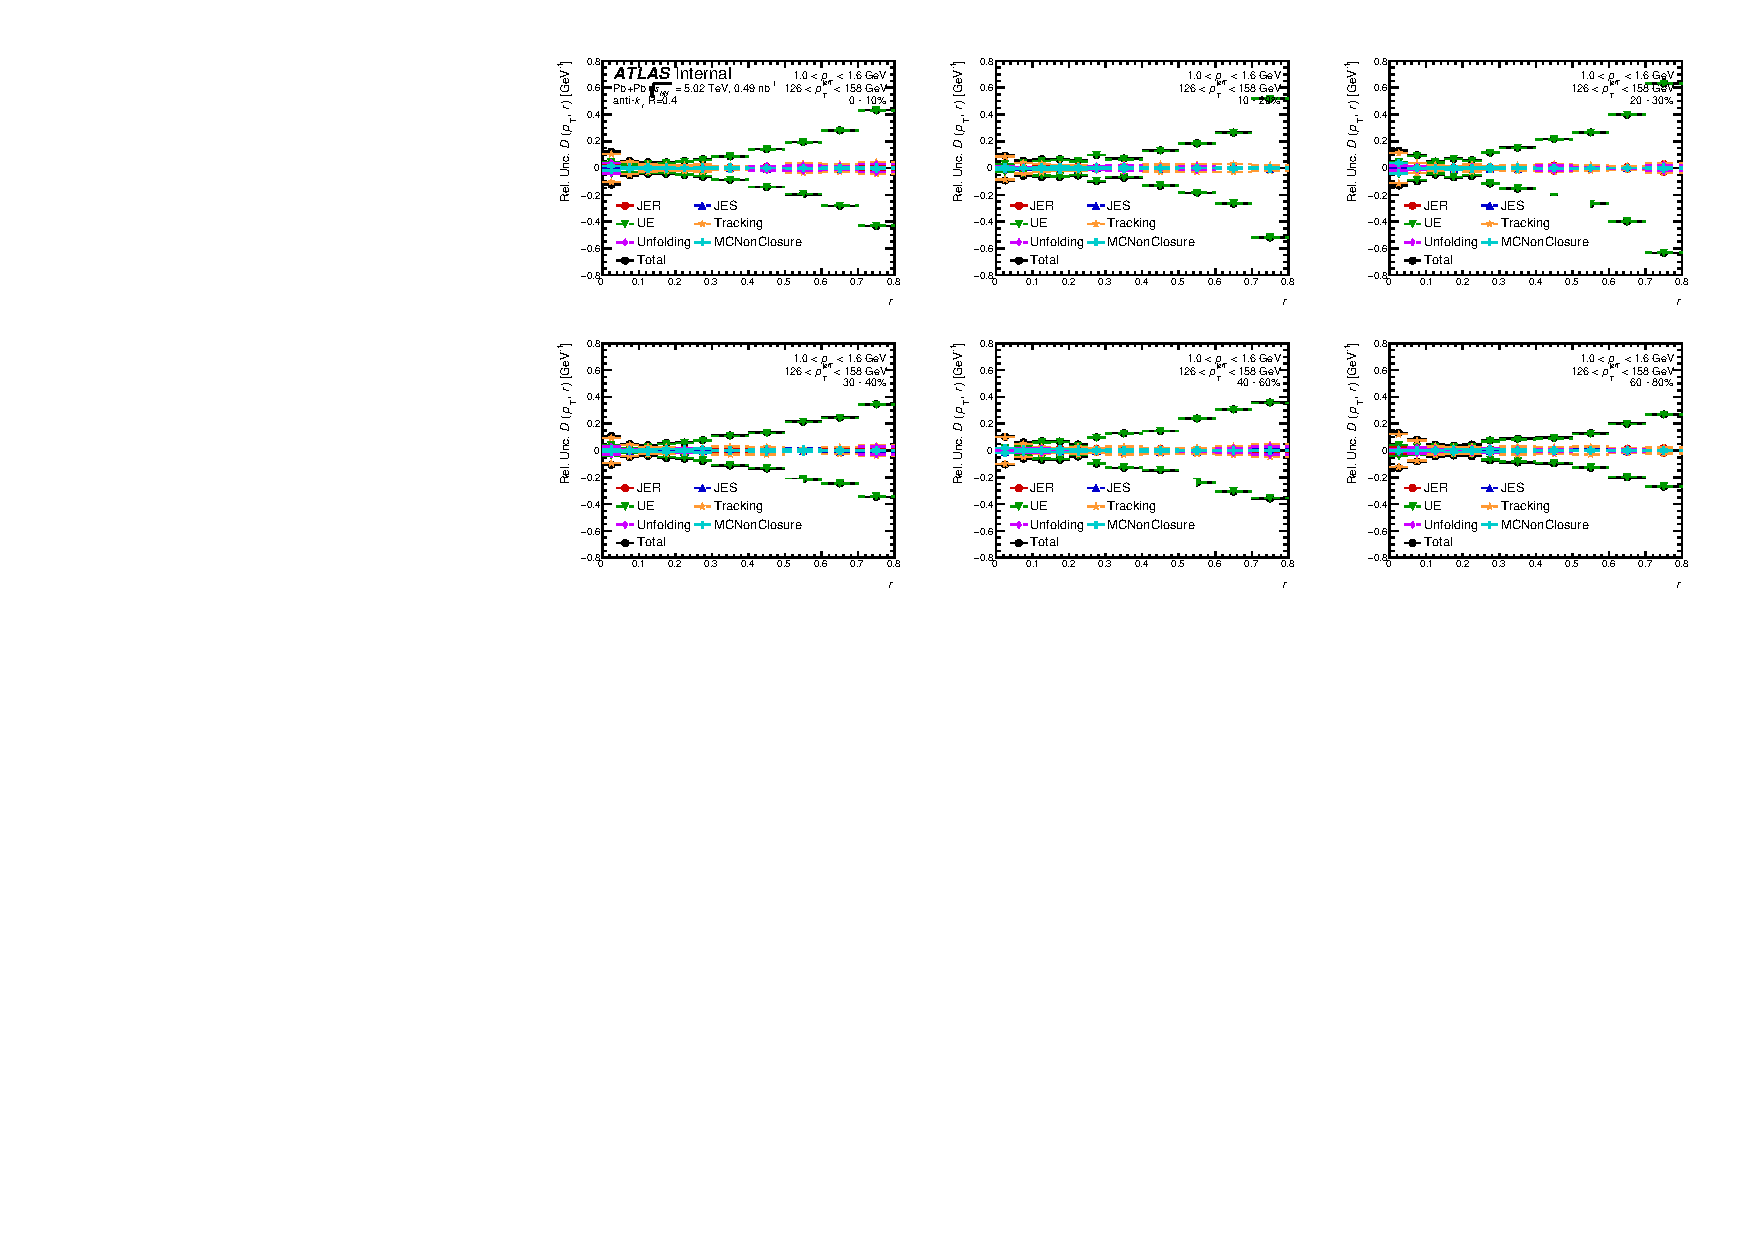
\includegraphics[page=1, width=\textwidth]{figures/main/figures_systematics/Summary_ChPS_dR_sys_PbPb_error}
%    \caption{}
%    \label{fig:rdptr_sys_uncert1a}
%\end{subfigure} \\
%\begin{subfigure}[b]{\textwidth}
%    \centering
%    \includegraphics[page=3, width=\textwidth]{figures/main/figures_systematics/Summary_ChPS_dR_sys_PbPb_error}
%    \caption{}
%    \label{fig:rdptr_sys_uncert1b}
%\end{subfigure}\hfill
%   \caption{A summary of the systematic uncertainties on \RDptr\ distributions for different track \mbox{$1.0 < \pt < 1.6$ GeV} (\ref{fig:rdptr_sys_uncert1a}) and \mbox{$2.5 < \pt < 4.0$ GeV} (\ref{fig:rdptr_sys_uncert1b}), for jets with \pt\ 126--158 \GeV\ , as a function of \rvar\ for different centrality bins. Different panels are different centrality bins. The uncertainties from the JES, JER, UE, and Tracking  are shown, along with the total systematic uncertainty from all sources. }
%\label{fig:rdptr_sys_uncert1}
%\end{figure}
%

%\begin{figure}
%	\centering
%	\subfloat[ \label{a}]{{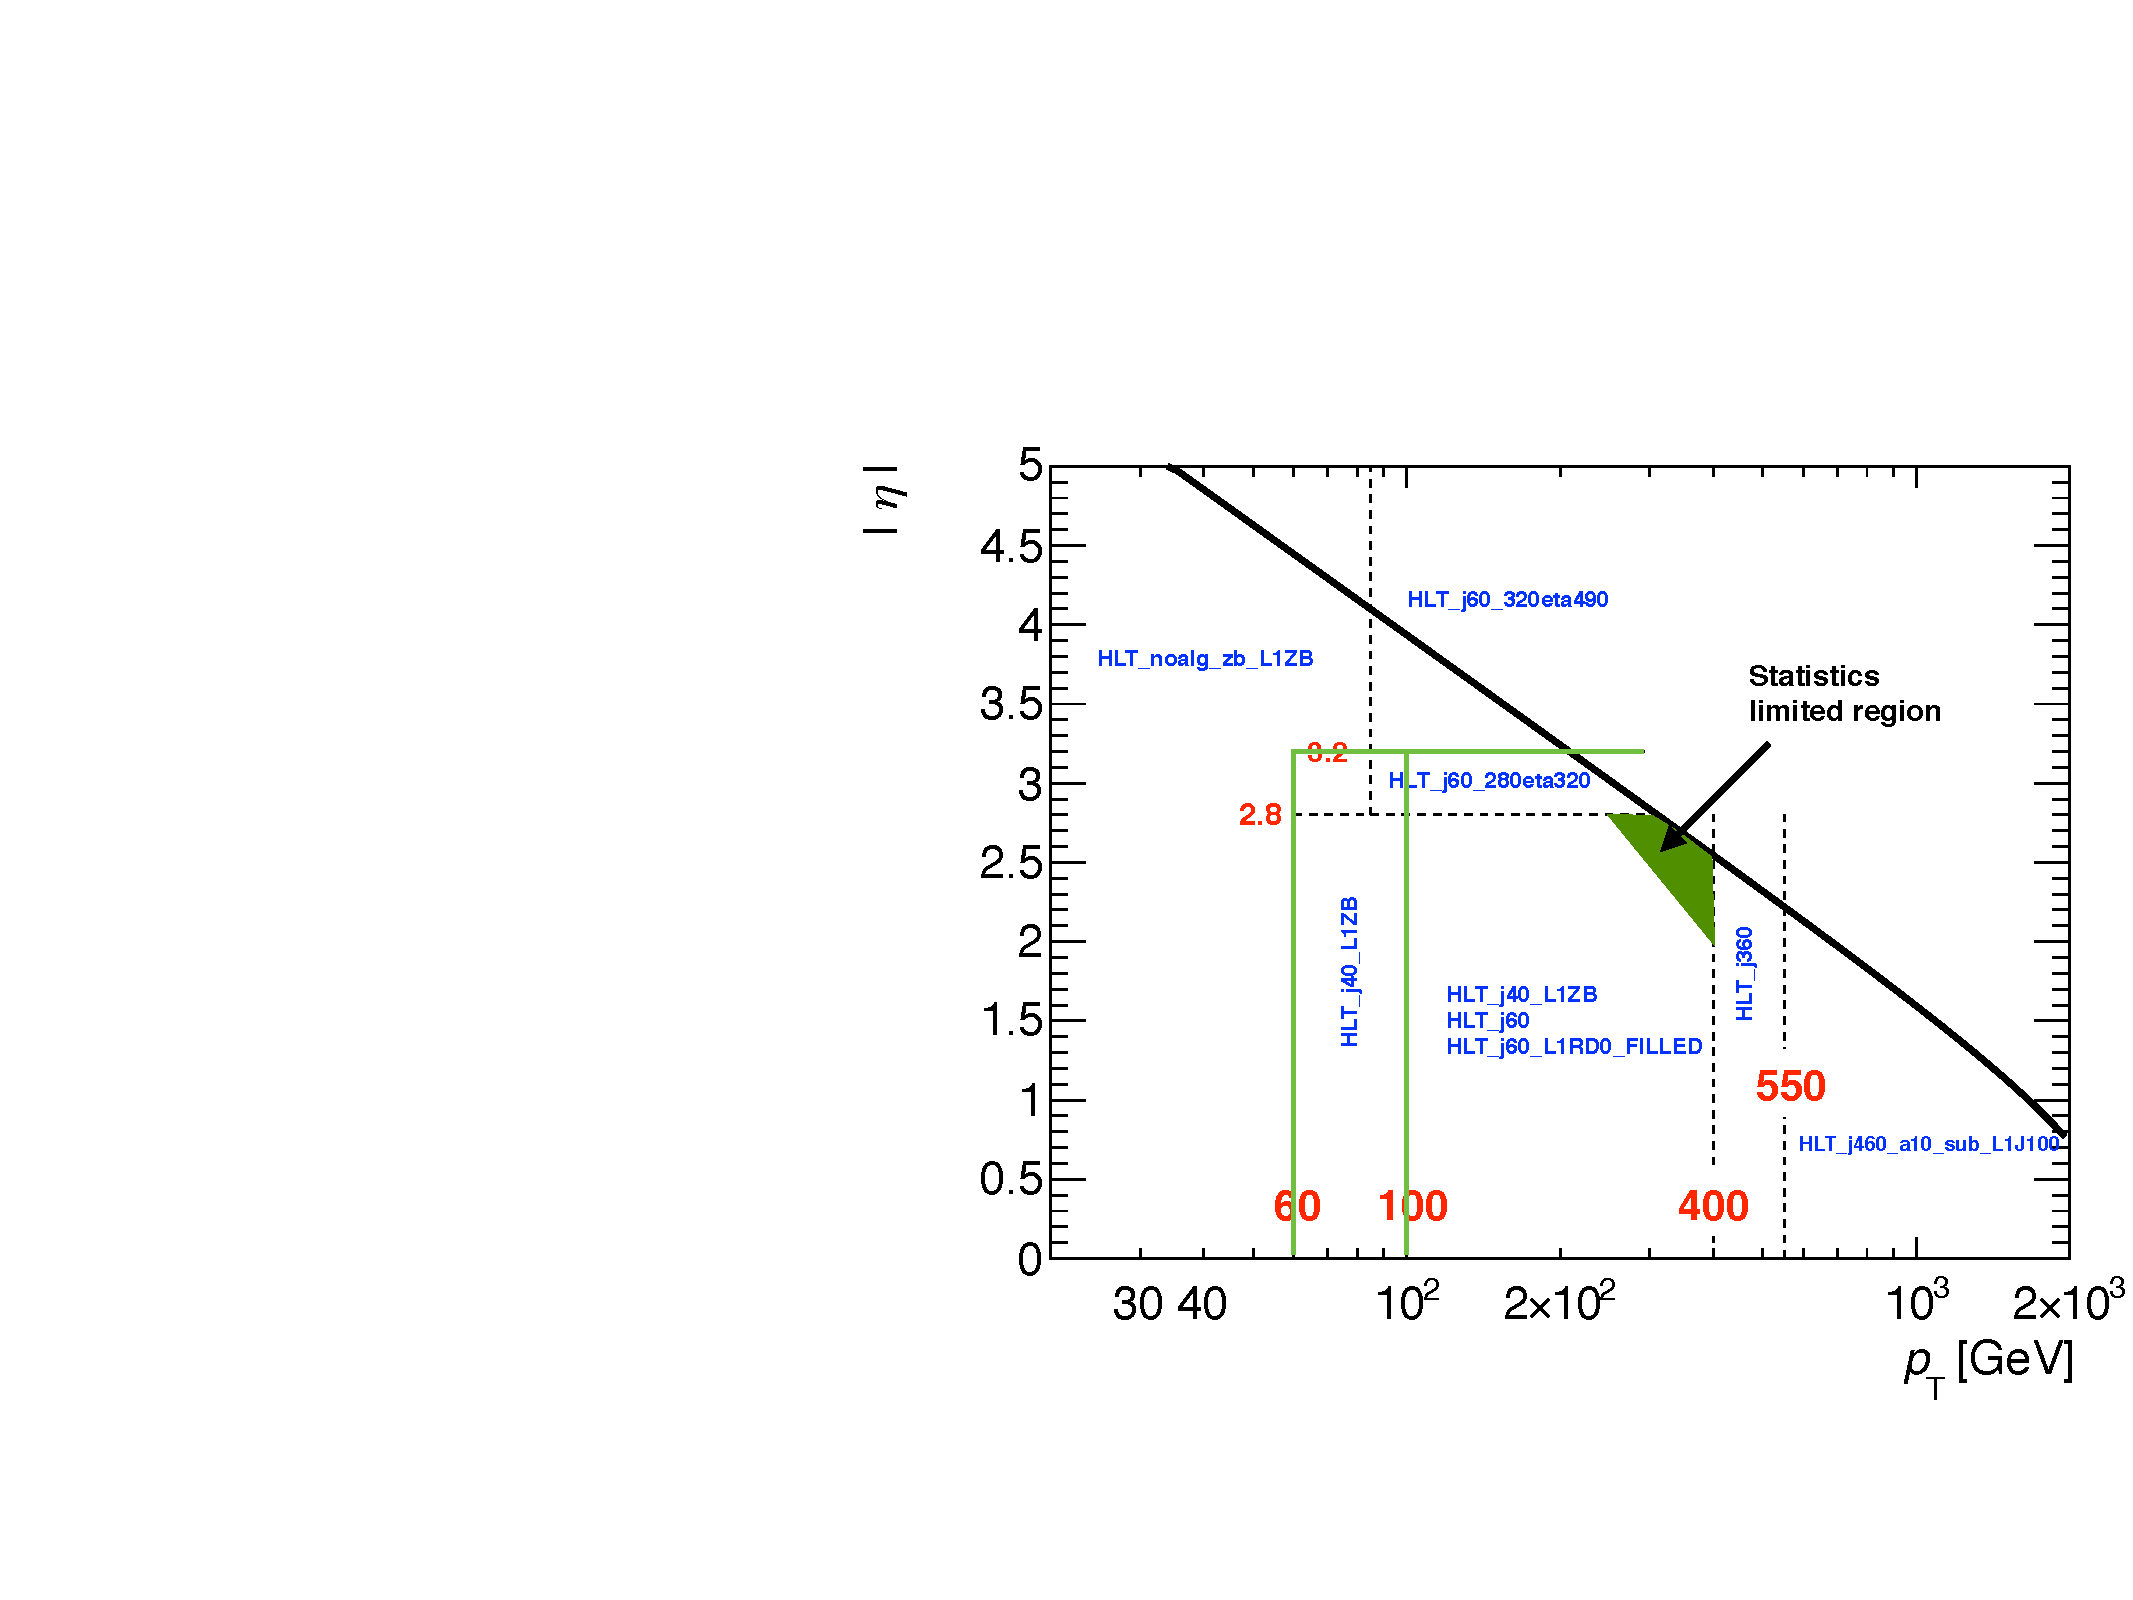
\includegraphics[width=0.5\textwidth]{figures/qualification/TrigMap.pdf} }}%
%	\subfloat[ \label{selection_2}]{{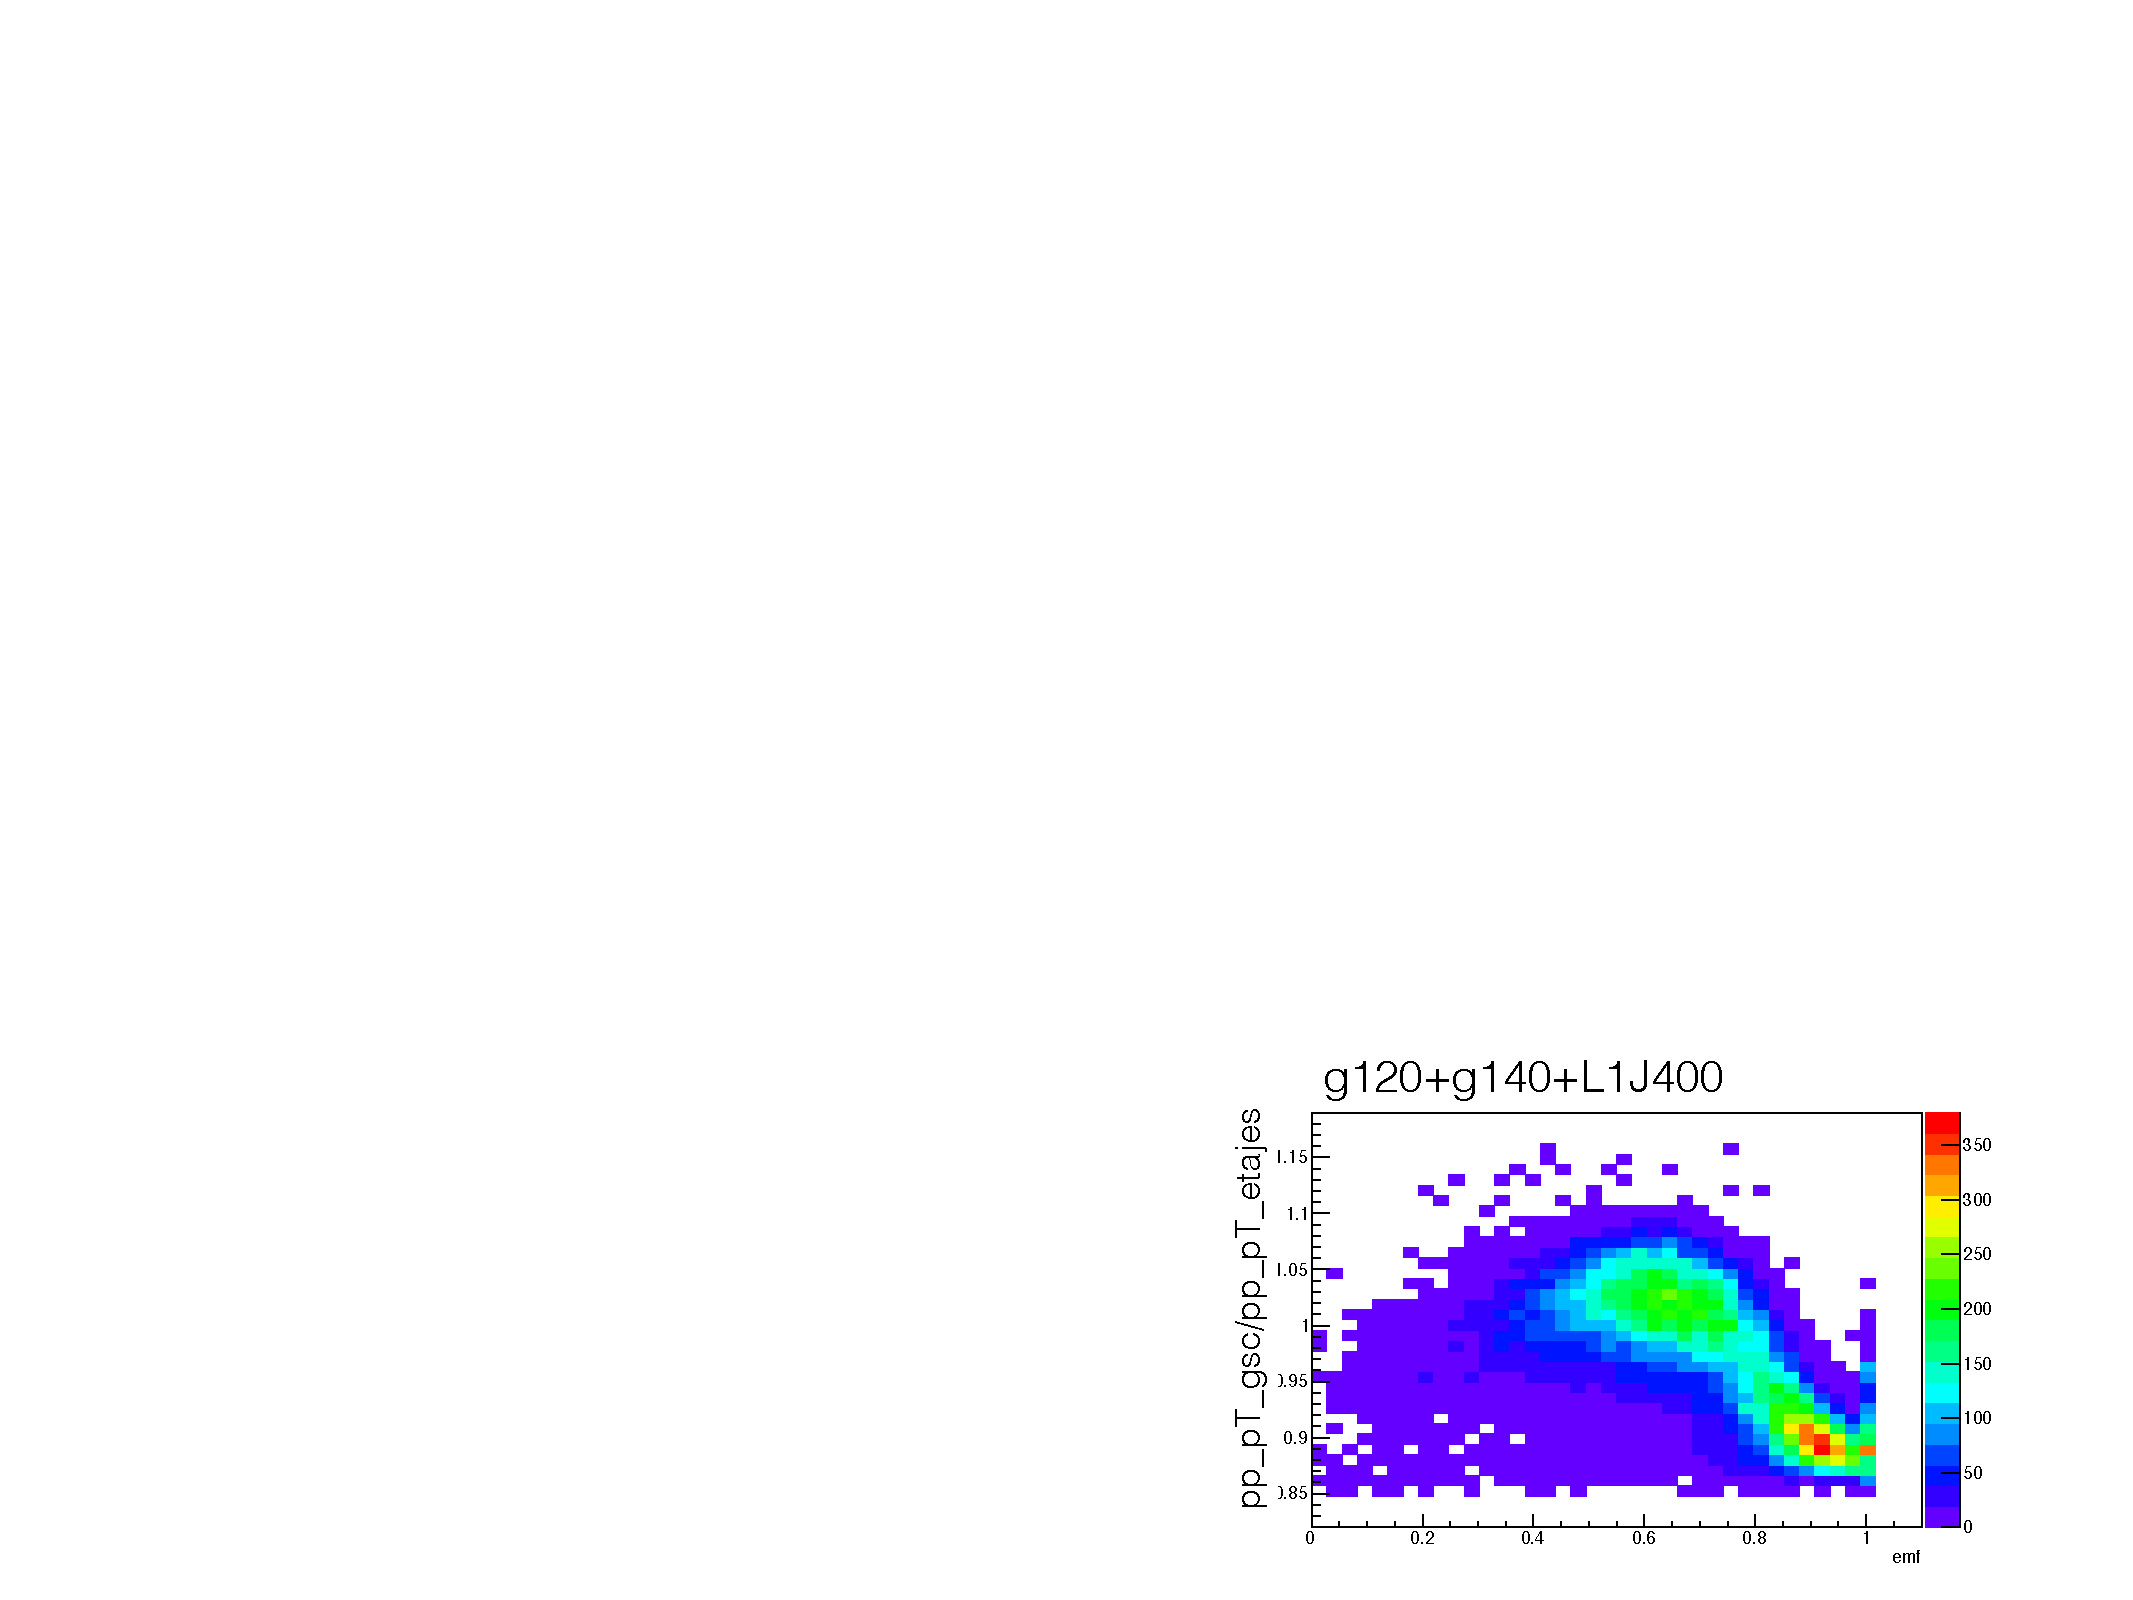
\includegraphics[width=0.5\textwidth]{figures/qualification/PhotonEx.pdf} }}%
%	\caption{The jet selection criteria in data based on different triggers. \protect\subref{a} $\pT-\eta$ phase space for different trigger regions used in the ZeroBias and express streams \protect\subref{b}The effect of the GSC calibration, as a function of the electromagnetic fraction (emf) of the jet. The peak at high emf is indicative of photons }%
%	\label{fig:TrigMap}%
%\end{figure}



\begin{figure}
\centering
\begin{subfigure}[b]{\textwidth}
    \centering
    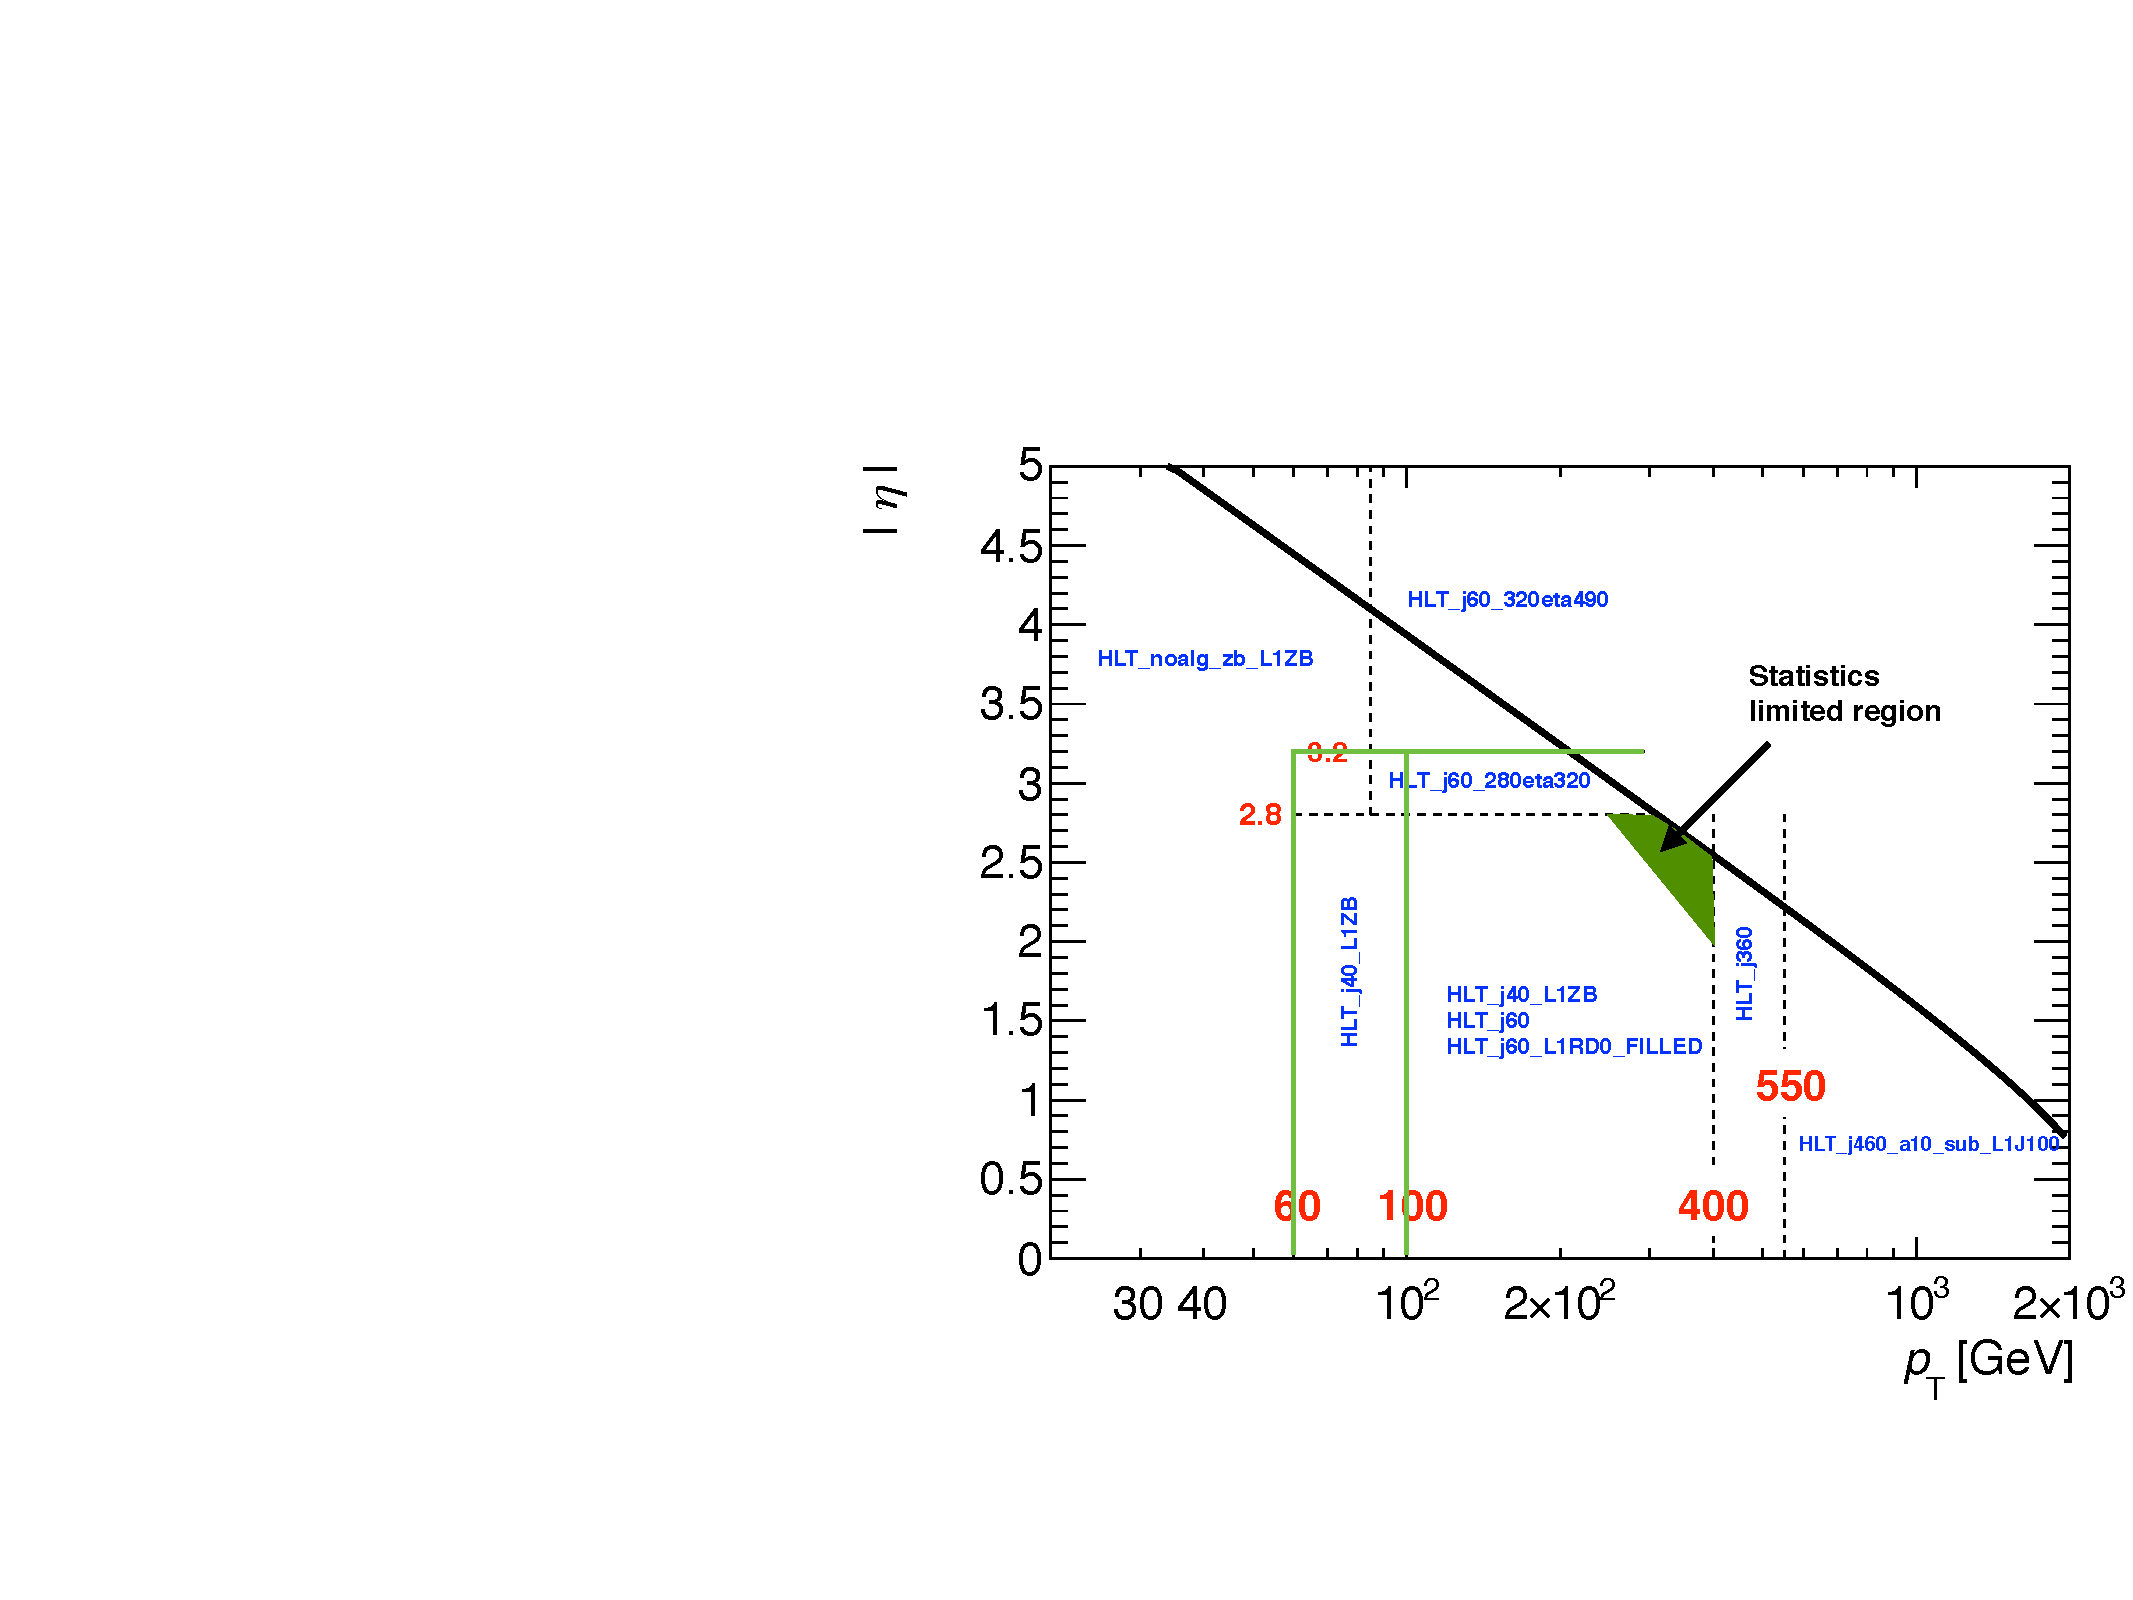
\includegraphics[width=\textwidth]{figures/qualification/TrigMap.pdf}
    \caption{}
    \label{a}
\end{subfigure} \\
\begin{subfigure}[b]{\textwidth}
    \centering
    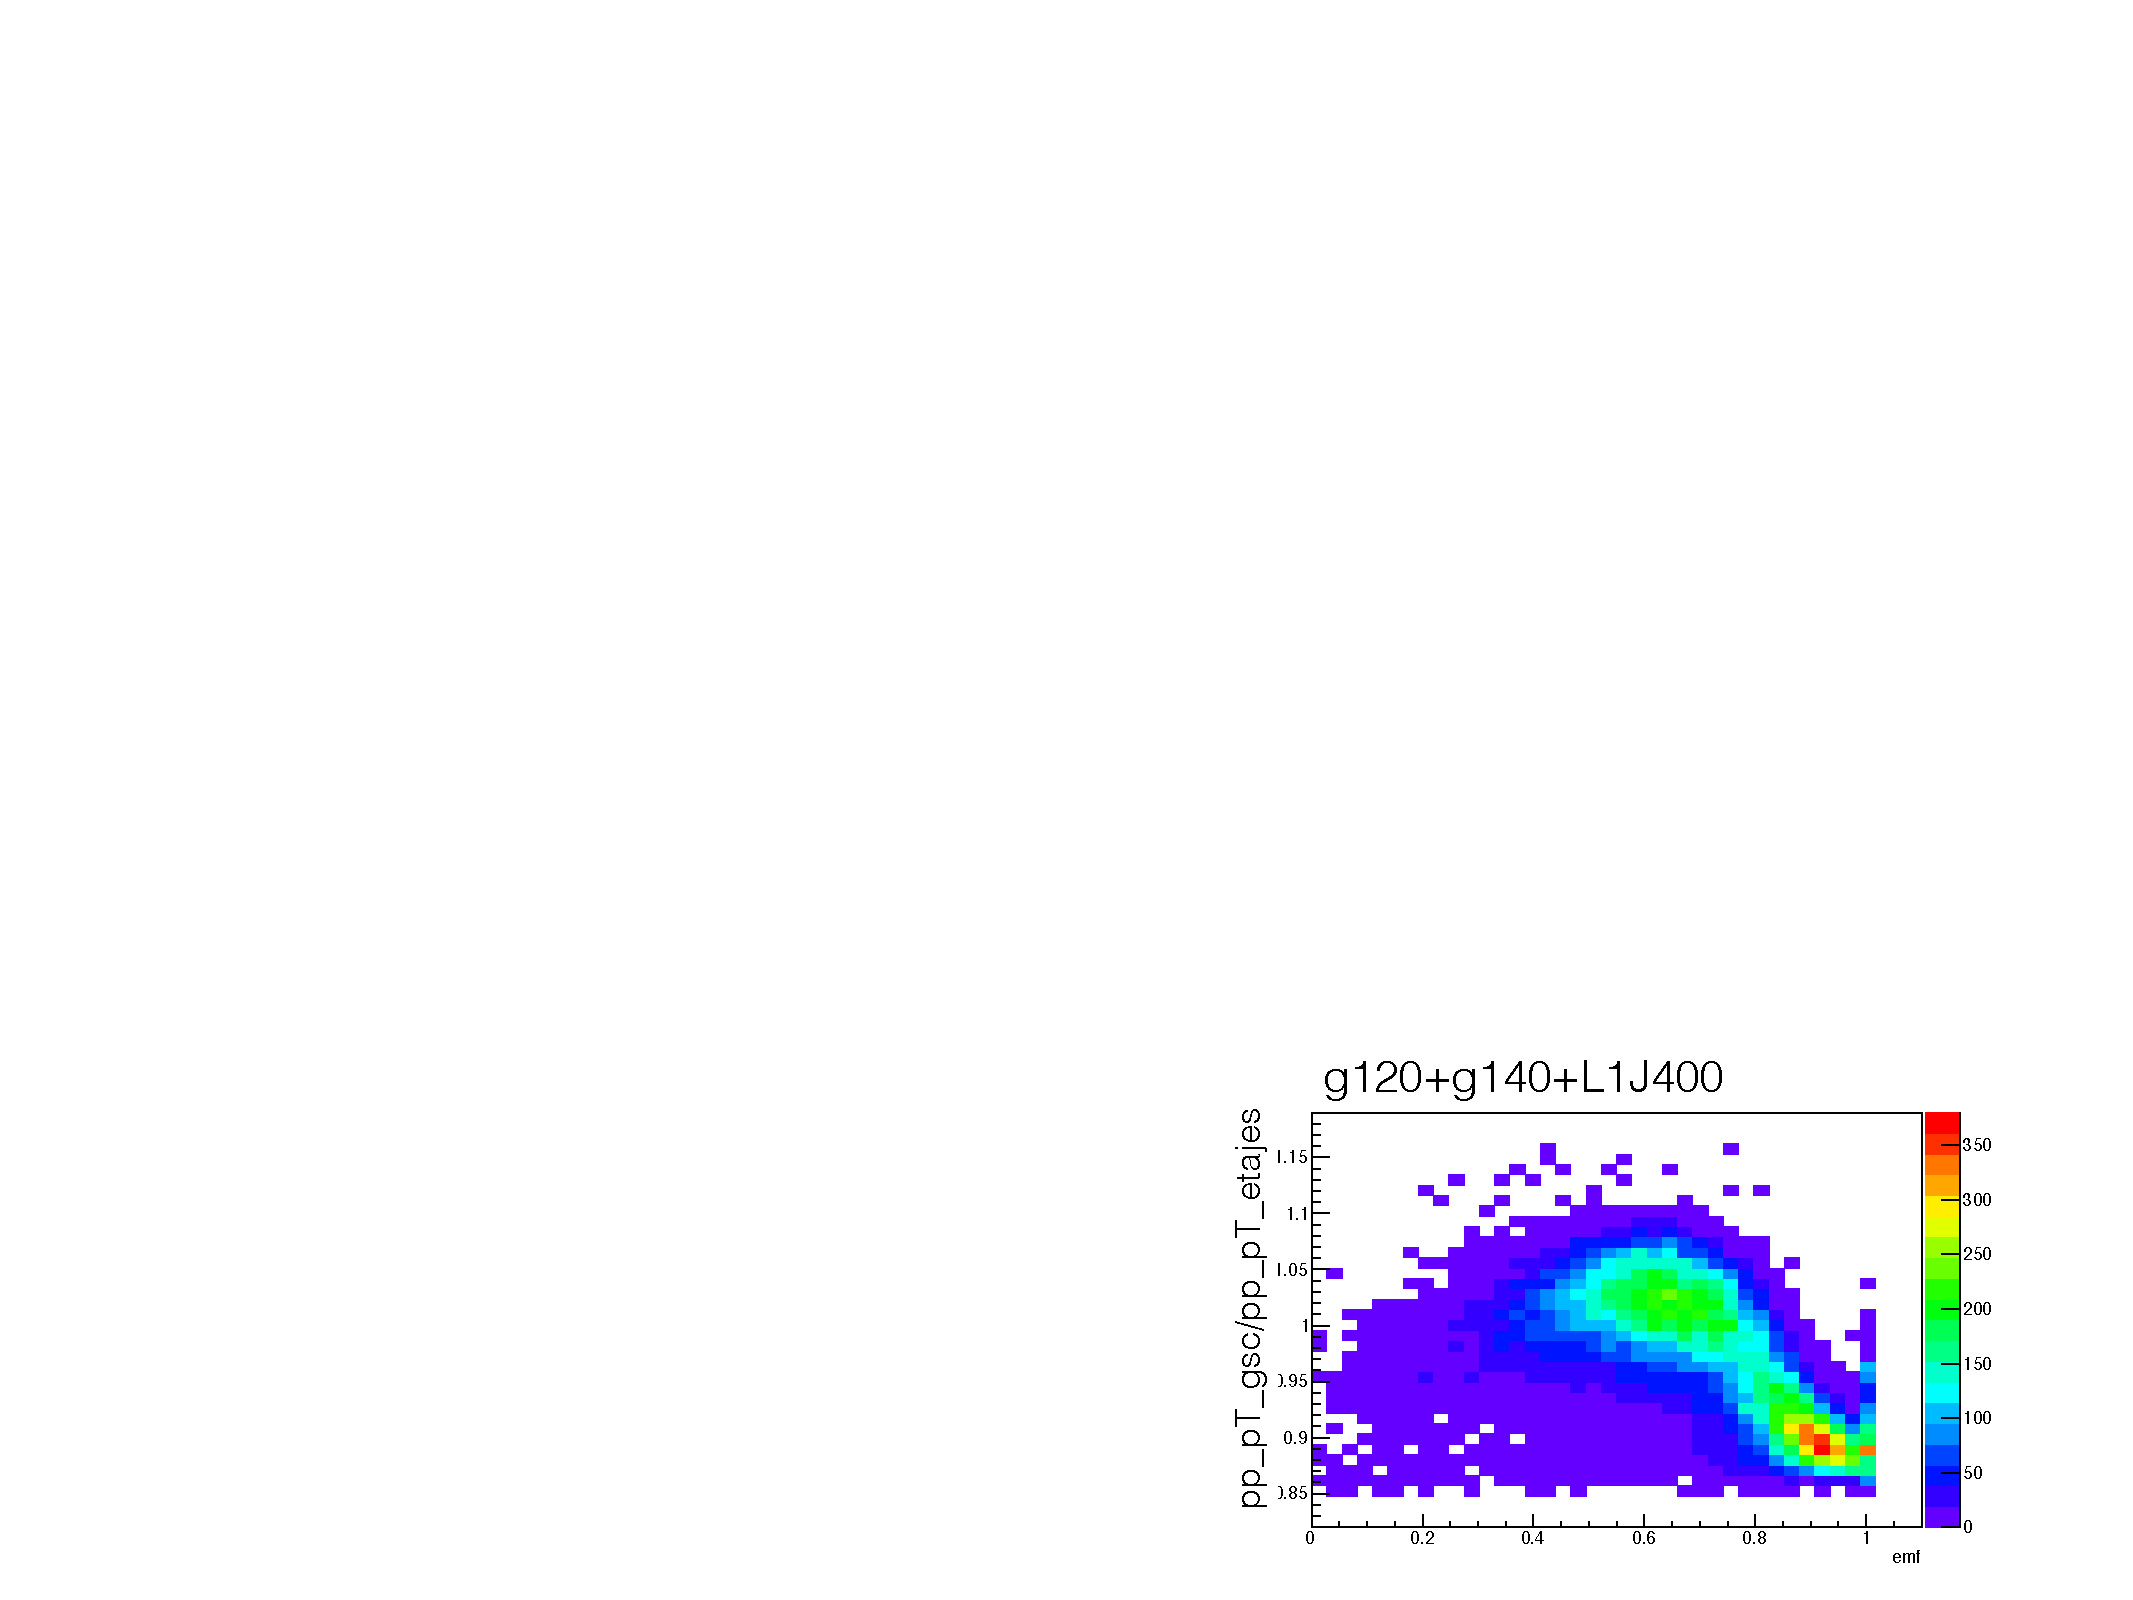
\includegraphics[width=\textwidth]{figures/qualification/PhotonEx.pdf}
    \caption{}
    \label{selection_2}
\end{subfigure}\hfill
   \caption{The jet selection criteria in data based on different triggers. \protect\subref{a} $\pT-\eta$ phase space for different trigger regions used in the ZeroBias and express streams \protect\subref{b}The effect of the GSC calibration, as a function of the electromagnetic fraction (emf) of the jet. The peak at high emf is indicative of photons }
\label{fig:TrigMap}
\end{figure}

Furthermore, events firing the HLT\_j360 trigger were vetoed if they also fired the HLT\_noalg\_L1J400, HLT\_g120\_loose, or the HLT\_g140\_loose. This was done to ensure that the jets entering the study were not in the wide turn on region of the aforementioned triggers. This also helped exclude photons (as can be seen in ~\ref{selection_2}.


MC events were filtered based on pileup. The MC generation settings included an average of combined 2015-2016 pileup profiles \cite{twiki_MC15c}. This can be seen in the top plot of Fig.~\ref{fig:mu_weight}, where the $\mu$ distribution in MC has a very wide spread, whereas the data (purely 2015) is localized around a central value. Events with $7 < \mu < 18$ were selected, and the jet $\pT$ in MC was weighted with the ratio $\mu_{\mathrm{Data}}/\mu_{\mathrm{MC}}$ (in addition to the eventweight present in JZXW MC samples).



\begin{figure}
	\centering
	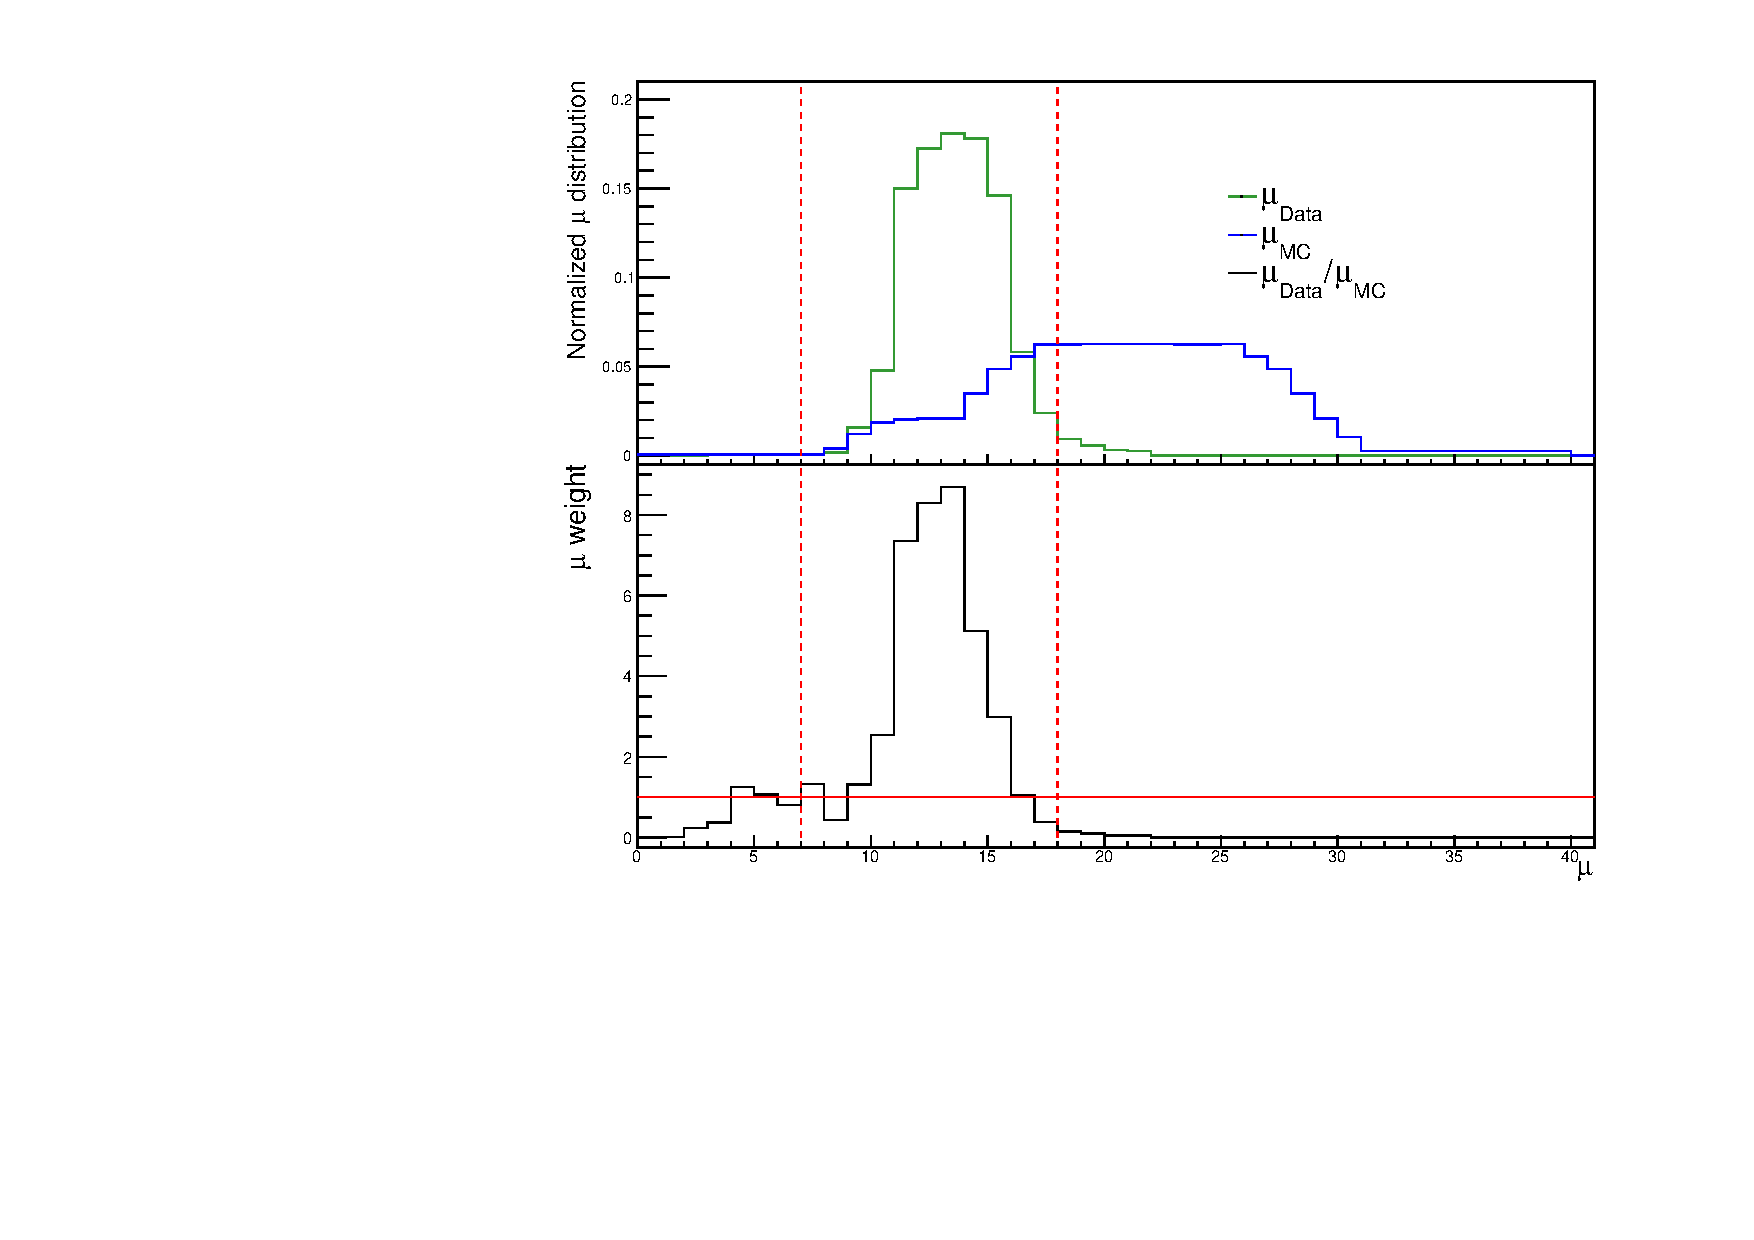
\includegraphics[width=1.0\textwidth]{figures/qualification/mu_weight.pdf}
	\caption{The top plot shows the normalized $mu$ distribution in data and MC. The bottom plot is a ratio of the two quantities. The jet selection criteria in MC is based on the pileup conditions. Events with $7 < \mu < 18$ were selected. }%
	\label{fig:mu_weight}%
\end{figure}

Other standard cuts included jet cleaning ({\it{LooseBad}} cut level with the option {\it{doUgly}} set to {\it TRUE}) and applying a GRL data15\_13TeV.periodAllYear\_DetStatus-v75-repro20-01\_DQDefects-00-02-02\_PHYS\_Standard\\GRL\_All\_Good\_25ns.xml)

The HI, EMTopo, and Truth jets were also isolated and matched to each other (and to truth in MC) with the criteria given in Tables~\ref{table:iso_criteria} and \ref{table:match_criteria}. The isolation \pt\ cut choice was dictated by the minimum\ \pT \ with which the HI and EMTopo jets are reconstructed (5 GeV for HI, 10 GeV for EMTopo). An investigation showed that for isolation $\pT$ cuts below 20 GeV, there was a large difference (upto at least a factor of ~2) in the number of EMTopo jets matched to truth jets, compared to HI jets matched to truth jets. The cross calibration factors were evaluated for jets with $30 < \pT < 1000 $ GeV.

\begin{table}[ht]
\caption{Isolation criteria used in the evaluation of the nominal cross calibration factors}
\centering
\begin{tabular}{c c c}
\hline\hline
Jet Collection & Radius cut & $\pT$ cut [GeV] \\ [0.5ex] % inserts table %heading
\hline
AntiKt4EMTopo & 1.0 & 20.0 \\ 
AntiKt4HI & 1.0 & 20.0 \\ 
Truth (in MC) & 0.6 & 20.0 \\ 
\hline
\end{tabular}
\label{table:iso_criteria}
\end{table}

\begin{table}[ht]
\caption{Matching criteria used in the evaluation of the nominal cross calibration factors}
\centering
\begin{tabular}{c c}
\hline\hline
Jet Collections & Radius cut \\ [0.5ex] % inserts table %heading
\hline
AntiKt4EMTopo + Truth & 0.2 \\ 
AntiKt4HI + Truth & 0.3 \\ 
AntiKt4(EMTopo+HI) & 0.4\\ 
\hline
\end{tabular}
\label{table:match_criteria}
\end{table}


%-------------------------------------------------------------------------------
\section{Procedure}
\label{sec:qual_procedure}
%-------------------------------------------------------------------------------

The results presented here were performed using the ATLAS detector and calorimeter systems ~\cite{Aad:2008zzm}. Jets with a radius of $R=0.4$ were reconstructed using the \\antikt \ algorithm.  The specifics of this procedure as applied to reconstruct the standard EMTopo jets and the HI jets are described in detail in \cite{Aad:pp_algo} and \cite{Aad:hi_jets} respectively. A brief summary is given below.

The EMTopo jets reconstruction involves using topological clusters of energy deposits in the calorimeter (calorimeter description in ~\cite{Aad:2008zzm}). The \\antikt \ algorithm \cite{antikt_algo}, as implemented in the FastJet sofware package \cite{fastjet_algo} is applied to these clusters, to reconstruct EMTopo jets with a $R = 0.4$.  The background in these jets, coming from the pile-up, is reduced by applying a $\pT$ and jet area dependent subtraction \cite{pp_pileup_subtr}. The jets are then calibrated using a energy and $\eta$ dependent calibration factor, derived from MC studies. The EMTopo jets for this study were calibrated up to MC based EtaJES, as described in \cite{CalibReco}.

The HI jet reconstruction also uses the anti-$k_{T}$ algorithm, but the inputs are $\Deta \times \Dphi = 0.1 \times \frac{\pi}{32}$ logical towers, deriving from the energy deposited in calorimeter cells. A fundamental difference between the reconstruction algorithms is how the underlying event (UE) is dealt with. The UE subtraction procedure involves the UE average tranvserse energy density ($\rho$), and the magnitude ($\nu_{2}$) and phase ($\Psi_{2}$) of the elliptic modulation from to flow. The subtraction applied to each cell within the jet is given as: 
\begin{align}
\Et^{\mathrm{subtr}} = \Et^{\mathrm{cell}} - \rho(\eta^{\mathrm{cell}},\phi^{\mathrm{cell}})A^{\mathrm{cell}} \{1 + 2\nu_{2 i}\cos[2(\phi - \Psi_2)]\}
\end{align}
where $\eta^{\mathrm{cell}}$ and $\phi^{\mathrm{cell}}$ are the cell coordinates, and $A^{\mathrm{cell}}$ is the cell area in $\eta-\phi$ space. $\Et^{\mathrm{subtr}}$ and $ \Et^{\mathrm{cell}}$ are the cell energies before and after subtraction \cite{HIjesnote}. The average UE transverse energy density is estimated from the cell transverse energies, whereas $\Psi_2$ is the determined from the FCal.
\begin{align}
\rho &\equiv \left\langle \frac{\Et^{\mathrm{cell}}}{A^{\mathrm{cell}}}\right\rangle \\
\Psi_2 &= \frac{1}{2} \tan^{-1}\frac{\sum \Et^{\mathrm{cell}} \sin 2\phi^{\mathrm{cell}} }{\sum \Et^{\mathrm{cell}} \cos 2\phi^{\mathrm{cell}} } \\
\nu_2 &= \frac{\sum \Et^{\mathrm{cell}} \cos 2(\phi^{\mathrm{cell}} - \Psi_2) }{\sum \Et^{\mathrm{cell}}}
\end{align}

The subtracted energy is seen to be independent of the jet\ \Et \ 

%IMPORTANT ----- insert subtracted pt figure here  ----- IMPORTANT


A summary of the differences between the EMTopo and HI jet reconstruction methods is given in Table \ref{table:algo_diff}.
\begin{table}[h]
\centering
\caption{A summary of the differences between the EMTopo and HI jet reconstruction algorithm. Adapted from \cite{HIjesnote}.}
\begin{tabular}{|c|c|c|}
\hline
            & EMTopo                 & HI                           \\ \hline
Inputs      & Topological clusters   & Calorimeter towers           \\ \hline
Subtraction & Median $\pT$ density & Average local energy density \\ \hline
\end{tabular}
\label{table:algo_diff}
\end{table}




The heavy ion jets were calibrated (upto {\it EtaJES}) using the procedure given in \cite{HICalib}, and the EMTopo jets were calibrated upto GSC (i.e. {\it JetArea\_Residual\_Origin\_EtaJES\_GSC}) using the ICHEP recommendations \cite{CalibReco}. This was done so that the cross calibration factors could be applied as a correction on top of the insitu correction. This allowed changing the insitu correction, without re-deriving the cross-calibration factors. 

A ratio of the EMTopo and HI jets, selected as described in Section~\ref{sec:datasets} was taken in both data and MC. The relative response and resolution in data and MC is shown in Fig.~\ref{fig:data_rel_resp} and \ref{fig:mc_rel_resp}. The distributions were calculated in the following $|\eta|$ bins: 0 - 0.3, 0.3 - 0.8, 0.8 - 1.2, 1.2 - 2.1, 2.1 - 2.8, 2.8 - 3.6, 3.6 - 4.4.

\begin{figure}[h]
\centerline{
         \begin{tabular}{cc}
            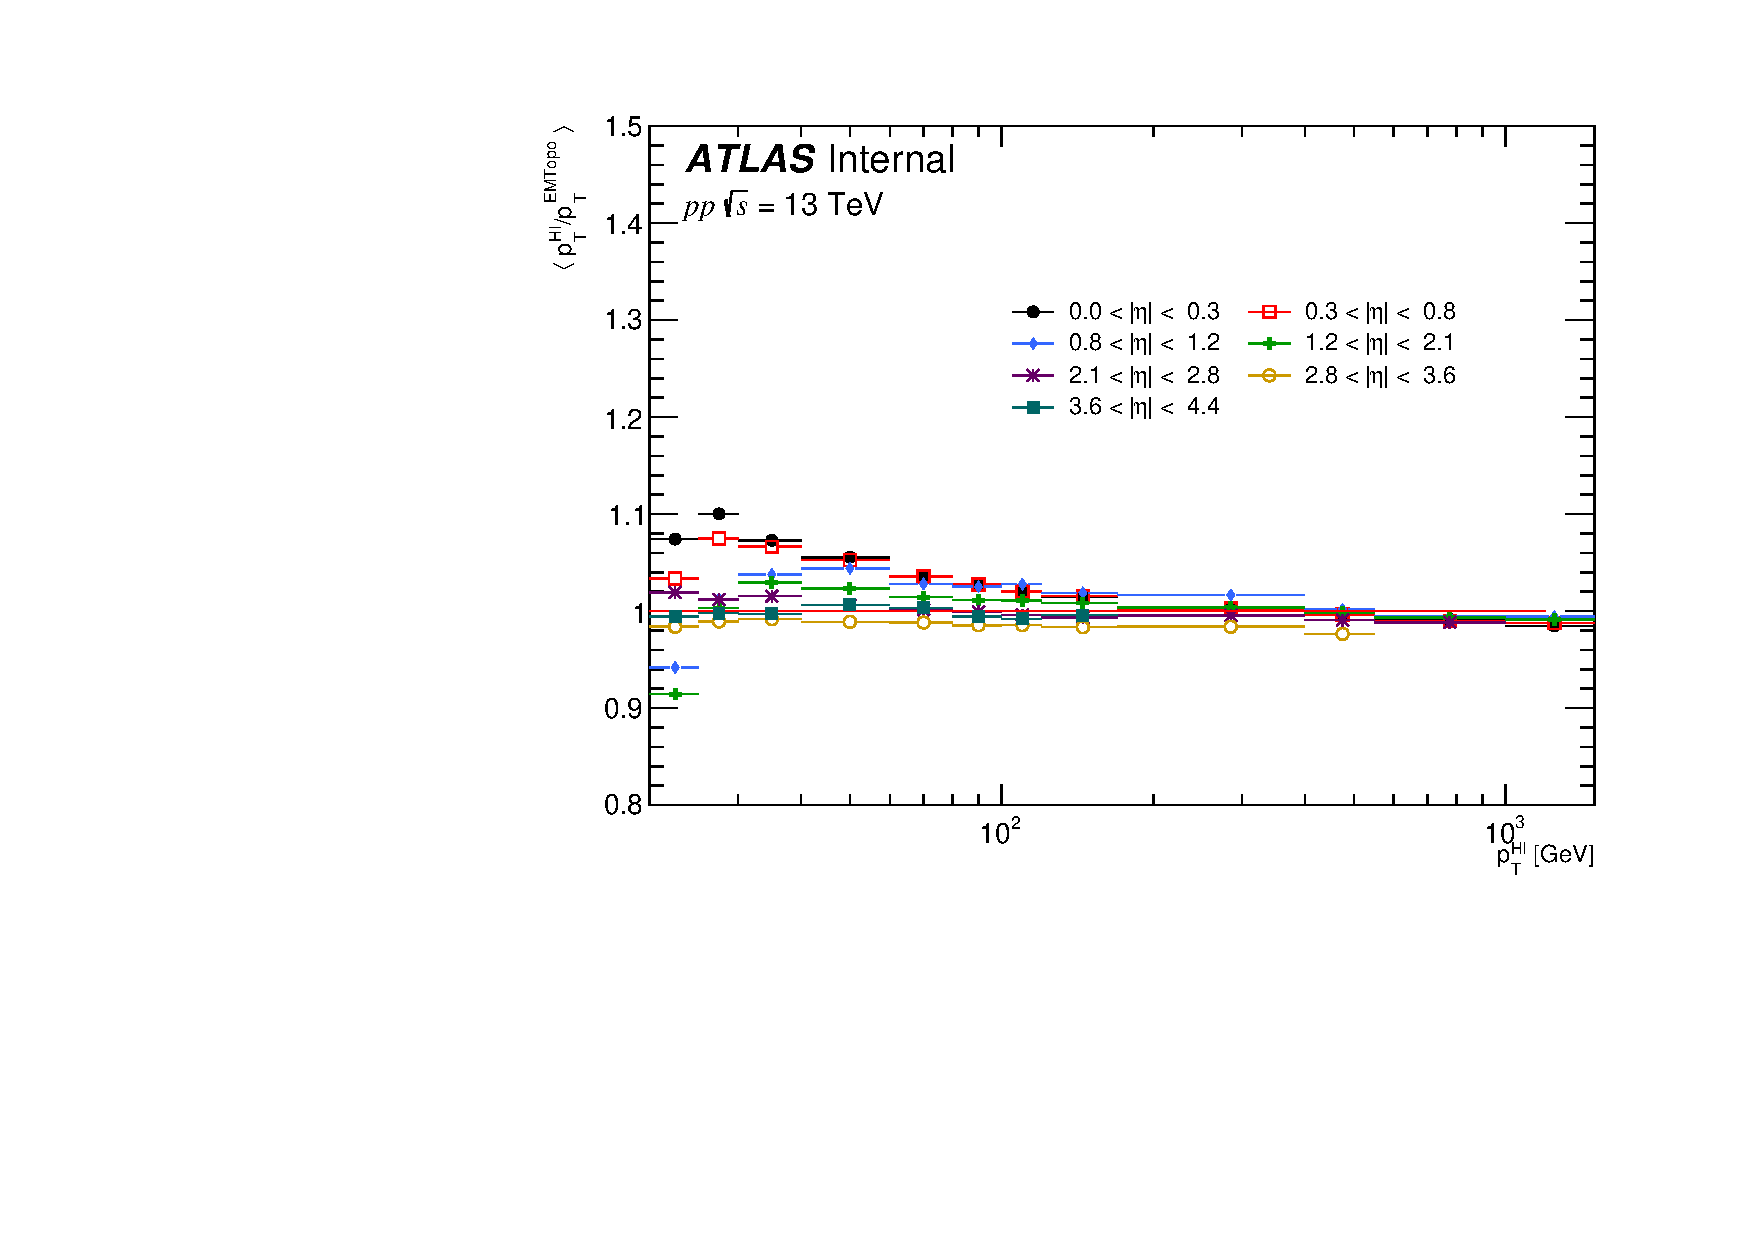
\includegraphics[width=0.5\textwidth]{figures/qualification/data_combined_h_resp12.pdf} & 
            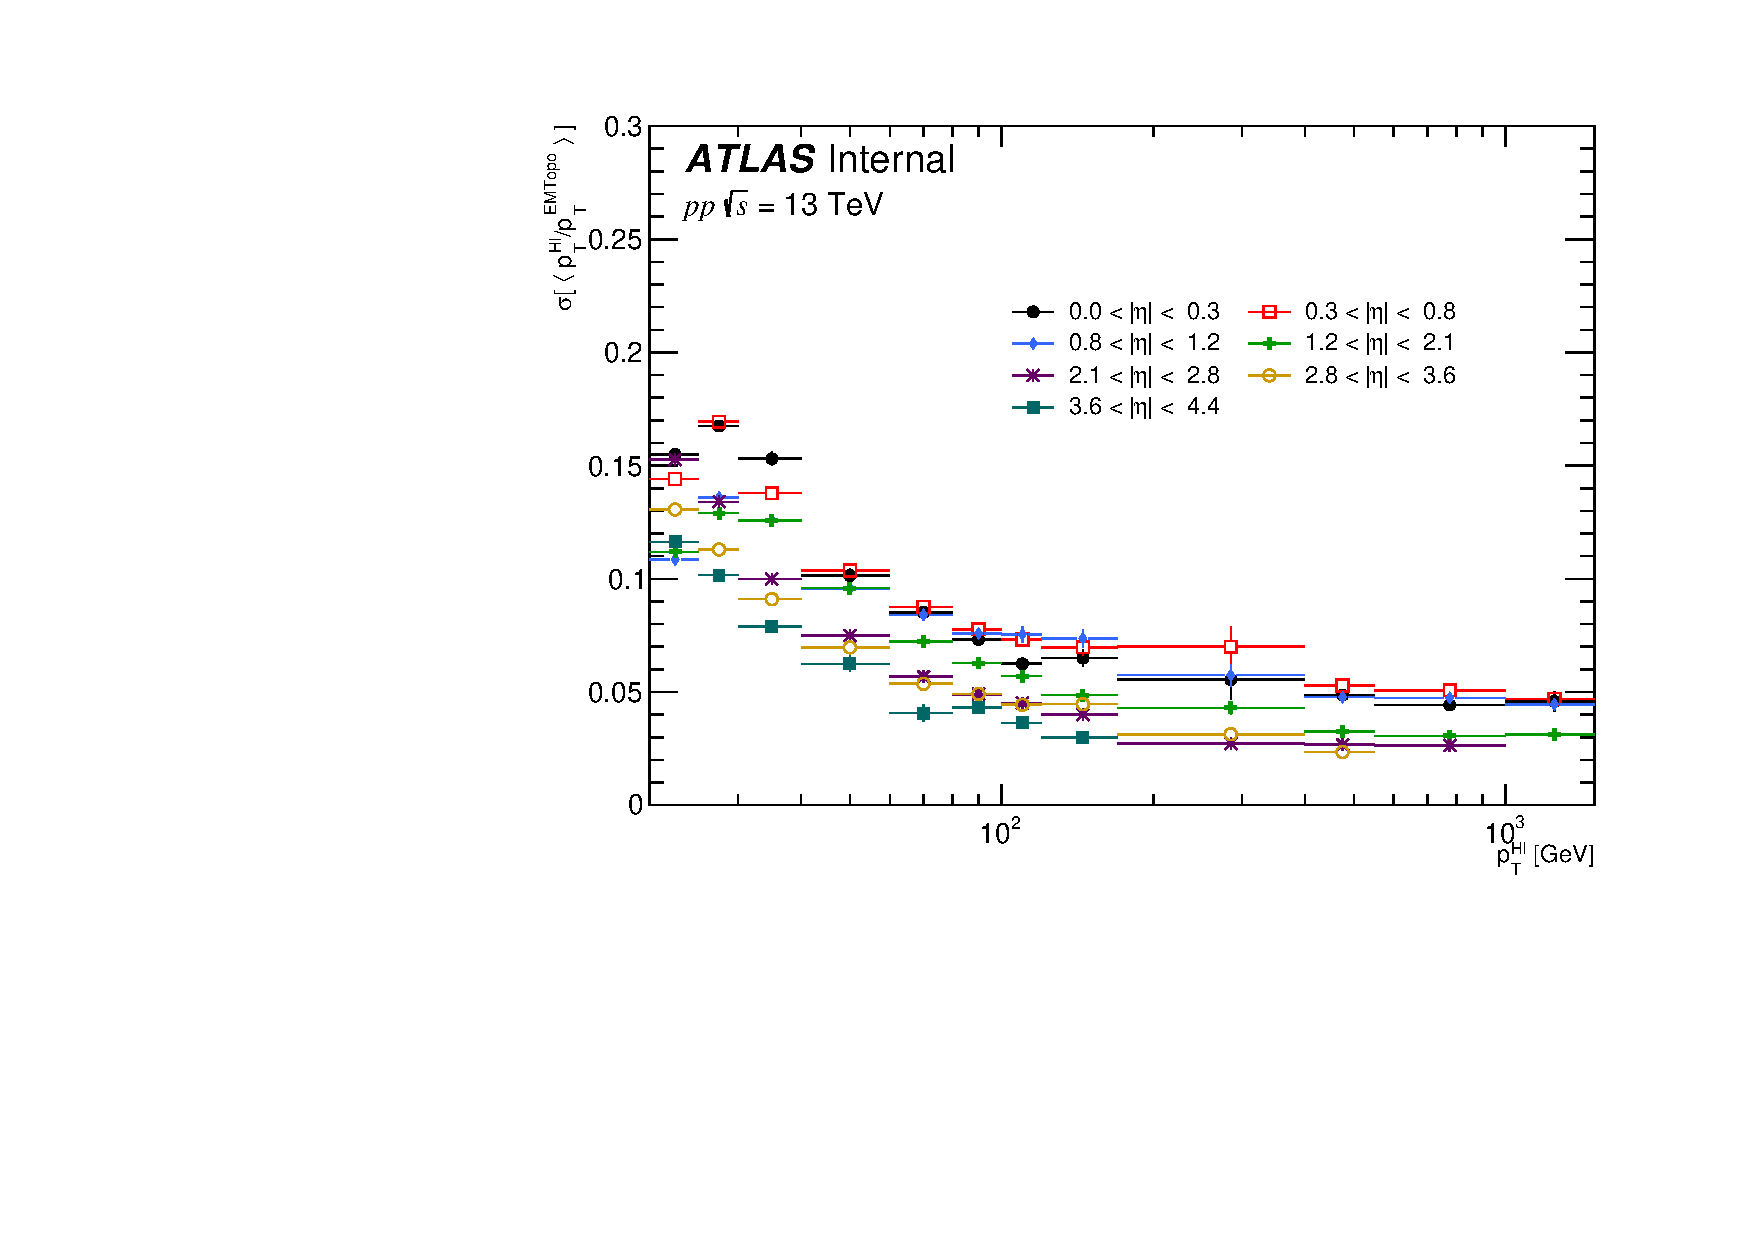
\includegraphics[width=0.5\textwidth]{figures/qualification/data_combined_h_resp12_jer.pdf} \\
      \end{tabular}
      }
\caption{The relative response (left) and relative resolution (right) in data, as a function of the HI jet $\pT$}
\label{fig:data_rel_resp}
\end{figure}

\begin{figure}[h]
\centerline{
         \begin{tabular}{cc}
            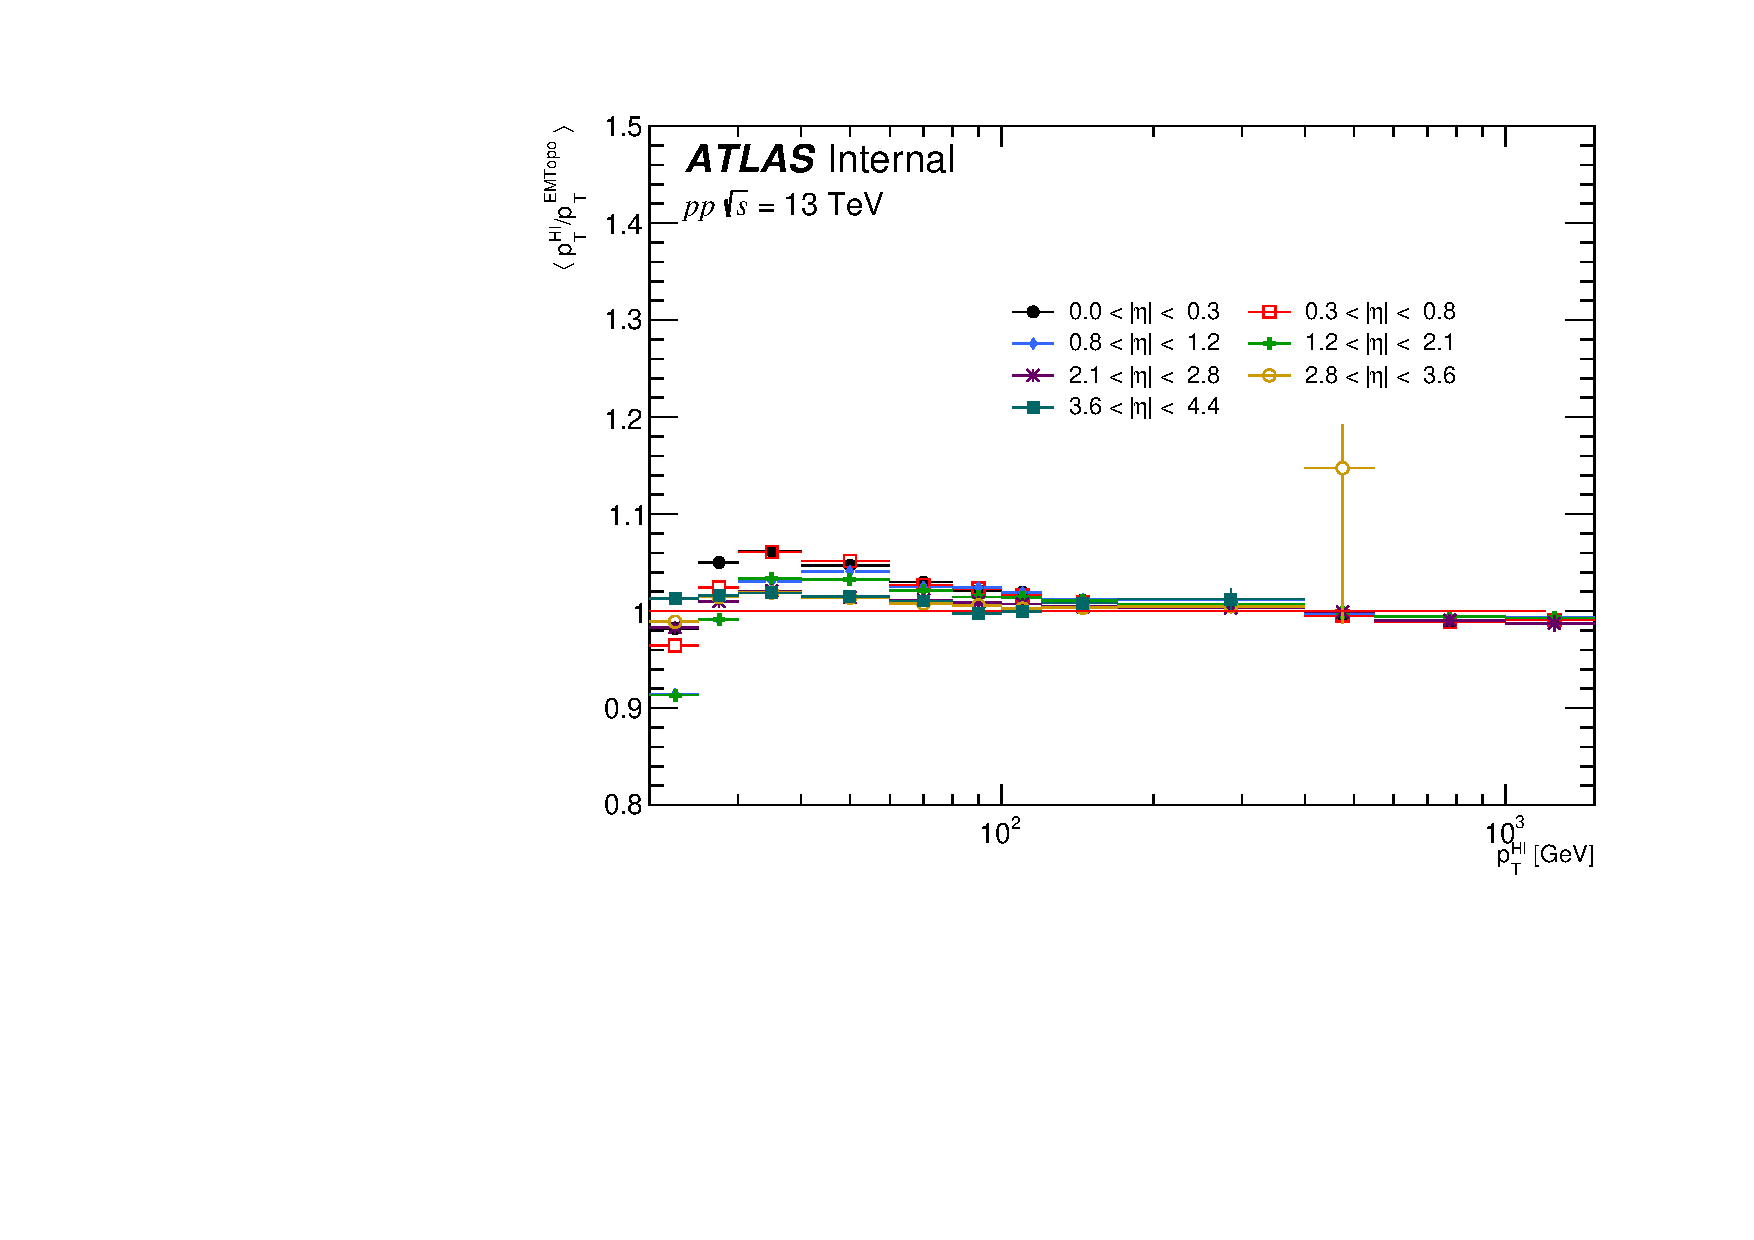
\includegraphics[width=0.5\textwidth]{figures/qualification/mc_combined_h_resp12.pdf} & 
            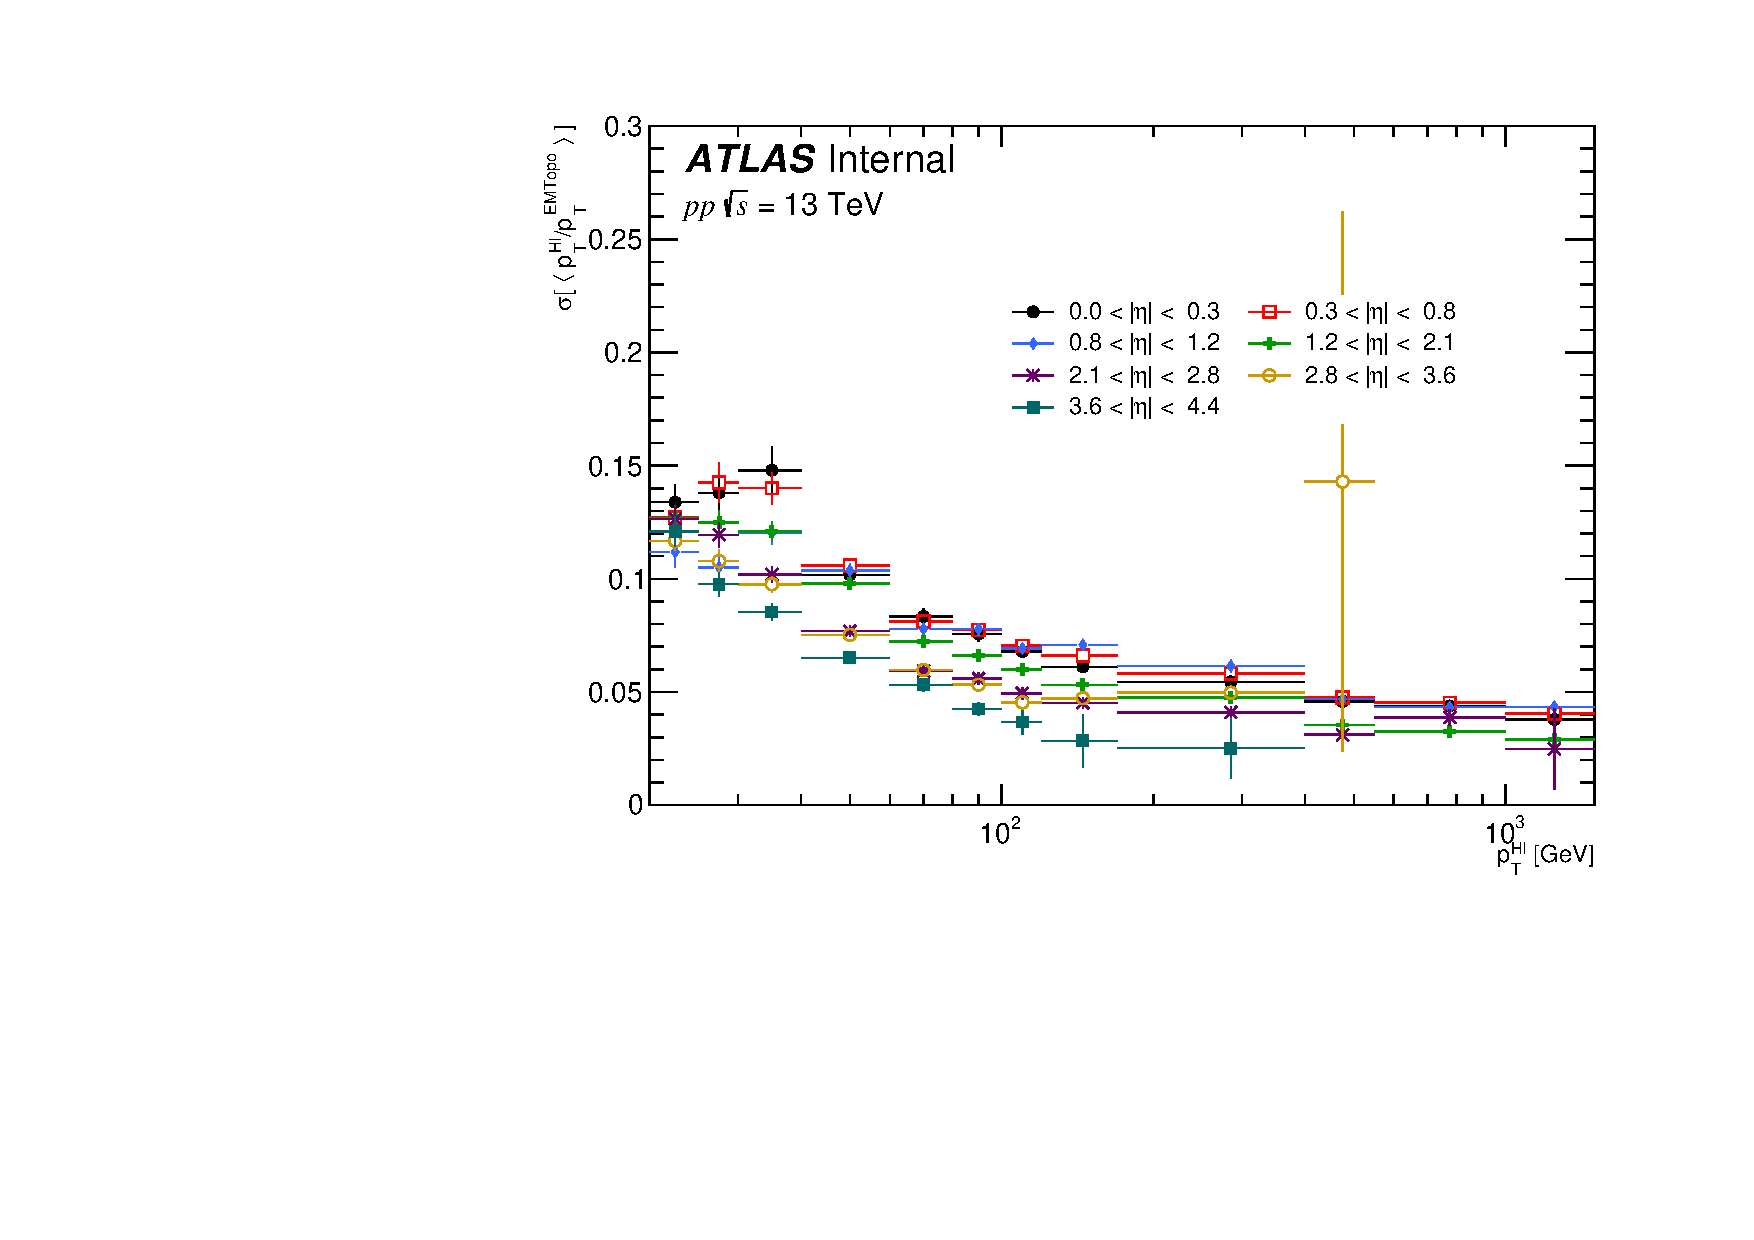
\includegraphics[width=0.5\textwidth]{figures/qualification/mc_combined_h_resp12_jer.pdf} \\
      \end{tabular}
      }
\caption{The relative response (left) and relative resolution (right) in MC, as a function of the HI jet $\pT$}
\label{fig:mc_rel_resp}
\end{figure}


The cross calibration factors, obtained by taking a ratio of the above relative response plots, were fit to a polynomial in log [$c_0 + c_1 \log(x) + c_2( \log(x))^2$] and are shown in Fig.~\ref{fig:cc_factors}. A ratio of the data to the fits is shown in Fig.~\ref{subfig:data2fit}.


\begin{figure}[h]
\centerline{
         \begin{tabular}{cc}
            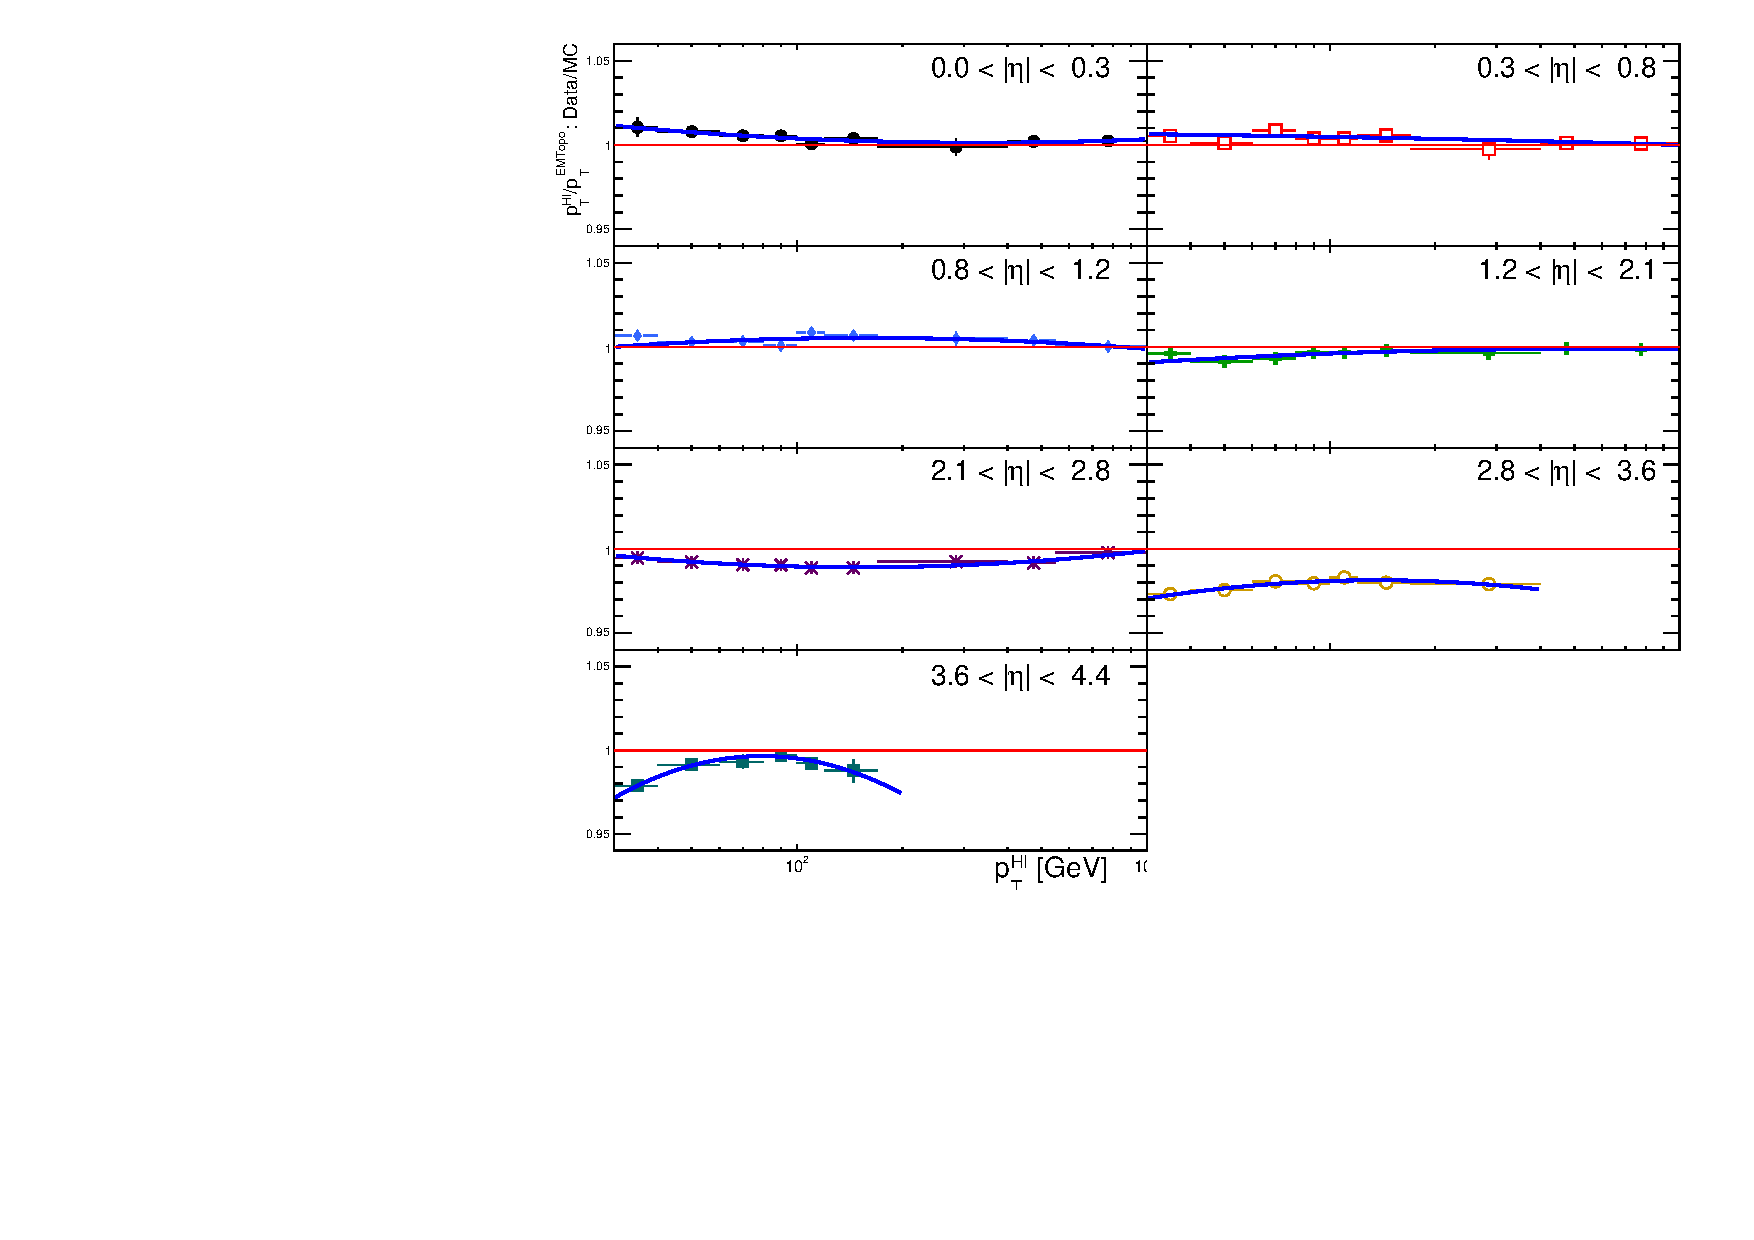
\includegraphics[width=0.5\textwidth]{figures/qualification/factors_w_fits} & 
            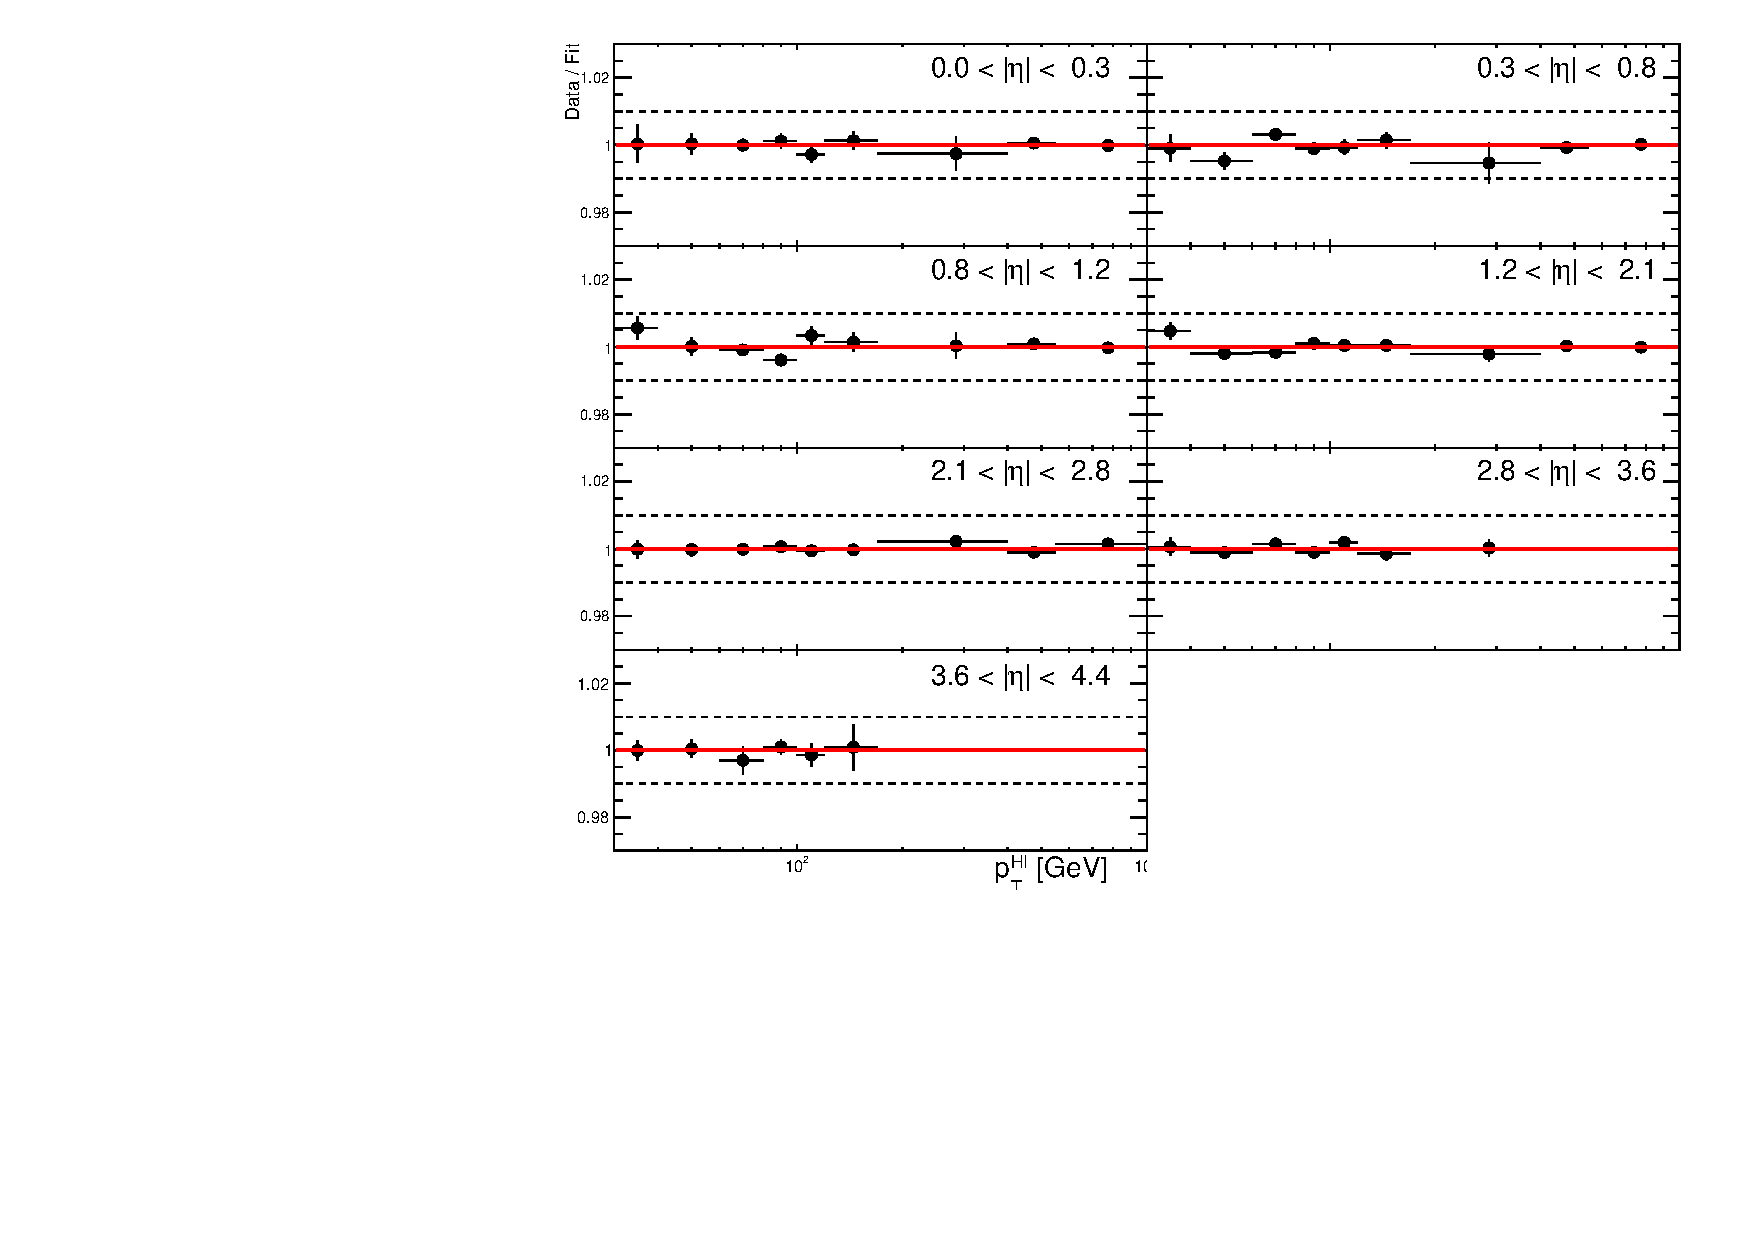
\includegraphics[width=0.5\textwidth]{figures/qualification/factors_data2fit} \\
      \end{tabular}
      }
\caption{The cross calibration factors, obtained from taking a ratio of the relative response in data and MC. A ratio of the data to the fit is given on the right}
\label{fig:cc_factors}
\end{figure}


%-------------------------------------------------------------------------------
\section{Uncertainties}
\label{sec:qual_uncertainties}
%-------------------------------------------------------------------------------

%---
\subsection{Cross calibration factor uncertainties}
\label{sec:qual_ccuncertainties}
%---


The statistical uncertainties come from the fits (using TVirtualFitter), whereas the systematics come from changing the parameters of the jet isolation criteria. These are summarized in Table~\ref{table:systematics_param}. Having a moderate nominal\ \pT \ cut on the isolation ensured that fluctuations in the HI reconstructed jets did not veto good jets. The \ \pT \ cut was also determined by the minimum\ \pT \ reconstructed by the reconstruction algorithms. The range of fits from this parametrization are shown in Fig.~\ref{fig:systematics}. The systematical uncertainties, evaluated as the maximum absolute difference between the nominal fit and any other iteration, are show in in Fig.~\ref{fig:sys_uncert}.

\begin{table}[h]
\caption{The isolation and matching parameters were varied to get the systematics. See Fig.~\ref{fig:systematics}}
\begin{tabular}{c c c c c c c c c c c}
\centering
 & \multicolumn{2}{c}{Nominal} & \multicolumn{2}{c}{Iteration 1} & \multicolumn{2}{c}{Iteration 2} & \multicolumn{2}{c}{Iteration 3} & \multicolumn{2}{c}{Iteration 4} \\
    \midrule
Isolation & R & \ \pT \ [GeV] & R & \ \pT \  [GeV] & R & \ \pT \ [GeV] & R & \ \pT \ [GeV] & \ \pT \ [GeV] \\
    \midrule
AntiKt4EMTopo		& 1.0 & 20.0 & 1.0 & 16.0 & 1.0 & 18.0 & 1.0 & 25.0 & 30.0\\
AntiKt4HI 			& 1.0 & 20.0 & 1.0 & 16.0 & 1.0 & 18.0 & 1.0 & 25.0 & 30.0\\
Truth  			& 0.6 & 20.0 & 0.6 & 16.0 & 1.0 & 18.0 & 0.6 & 25.0 & 30.0\\
    \bottomrule
    \label{table:systematics_param}
\end{tabular}
\end{table}

\begin{figure}
	\centering
	\subfloat{{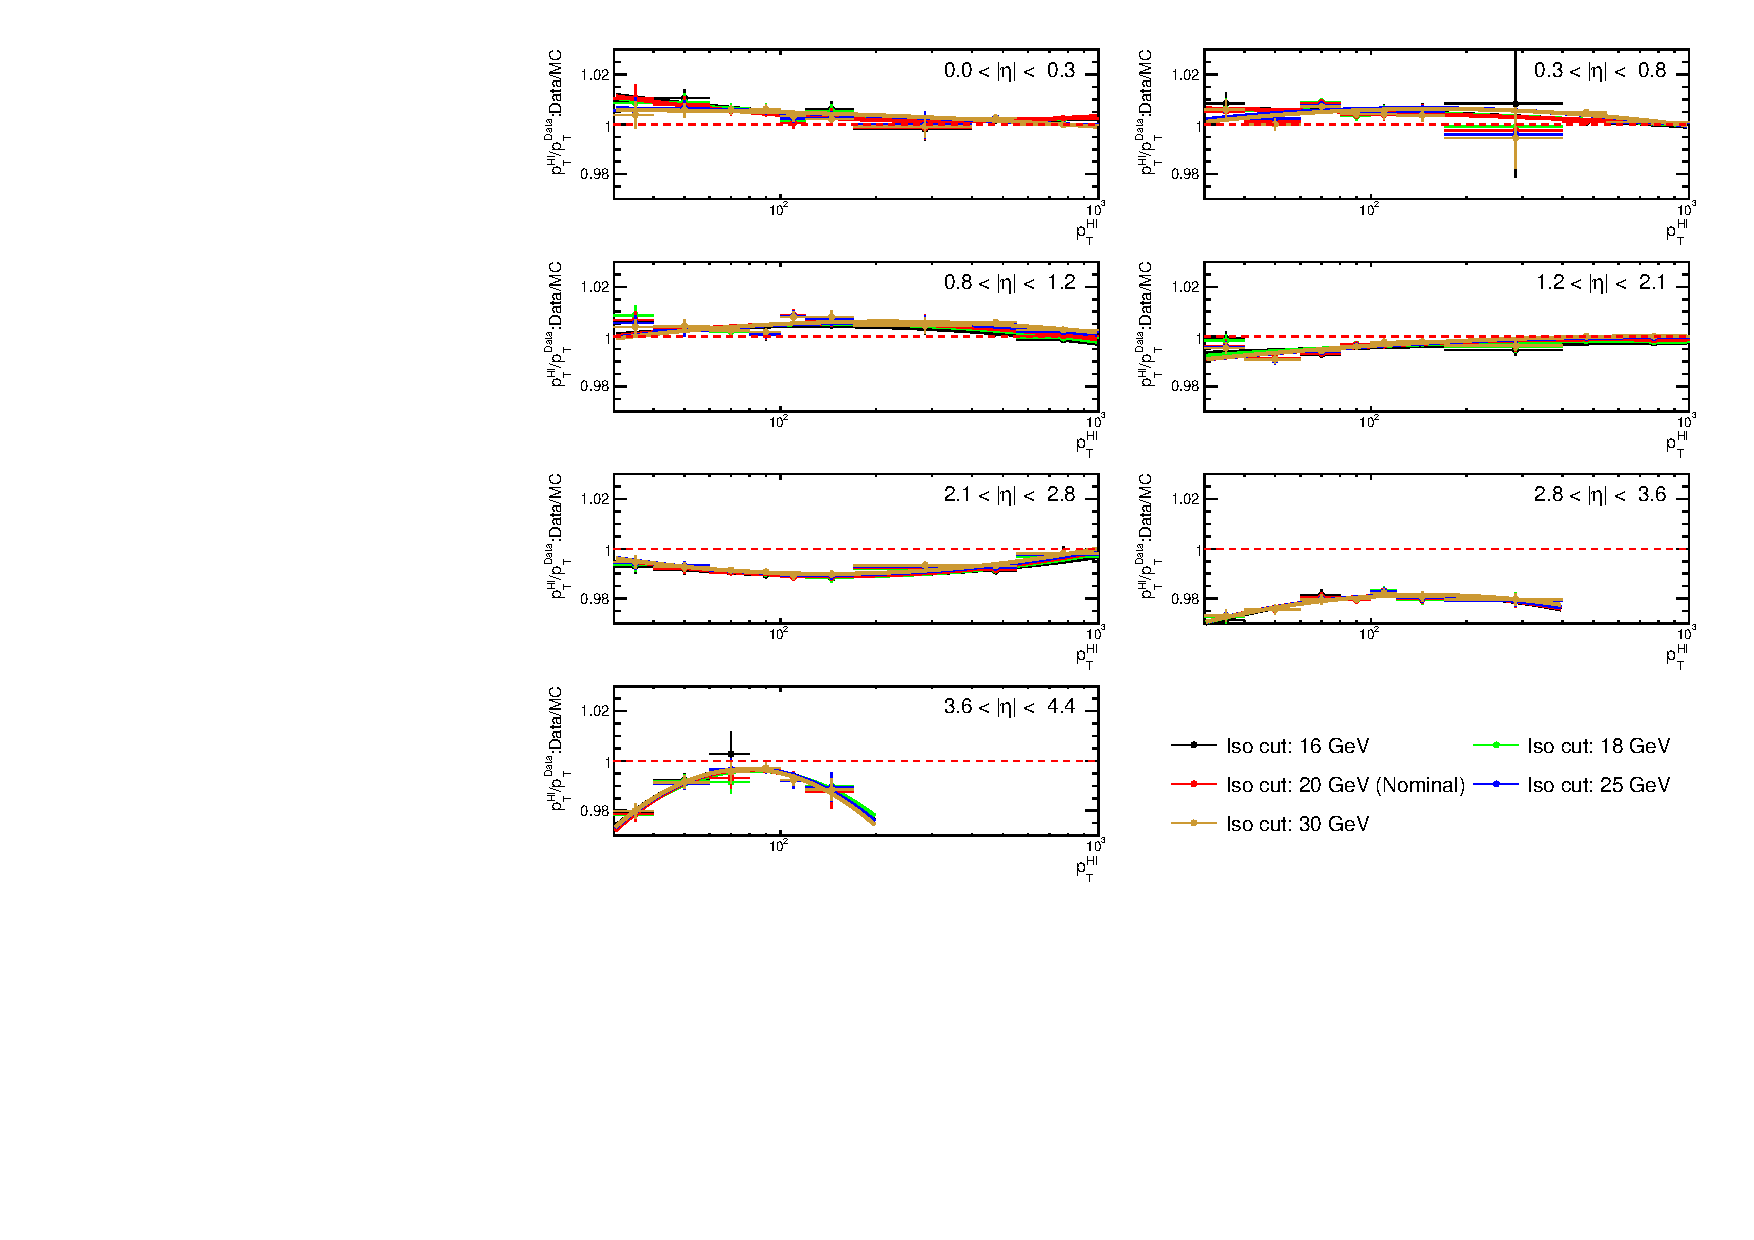
\includegraphics[width=1.0\textwidth]{figures/qualification/systematic_range} }}%
	\caption{The fits to the cross calibration factors, with different isolation/matching cuts, as specified in Table~\ref{table:systematics_param}.  }
	\label{fig:systematics}%
\end{figure}

\begin{figure}
	\centering
	\subfloat{{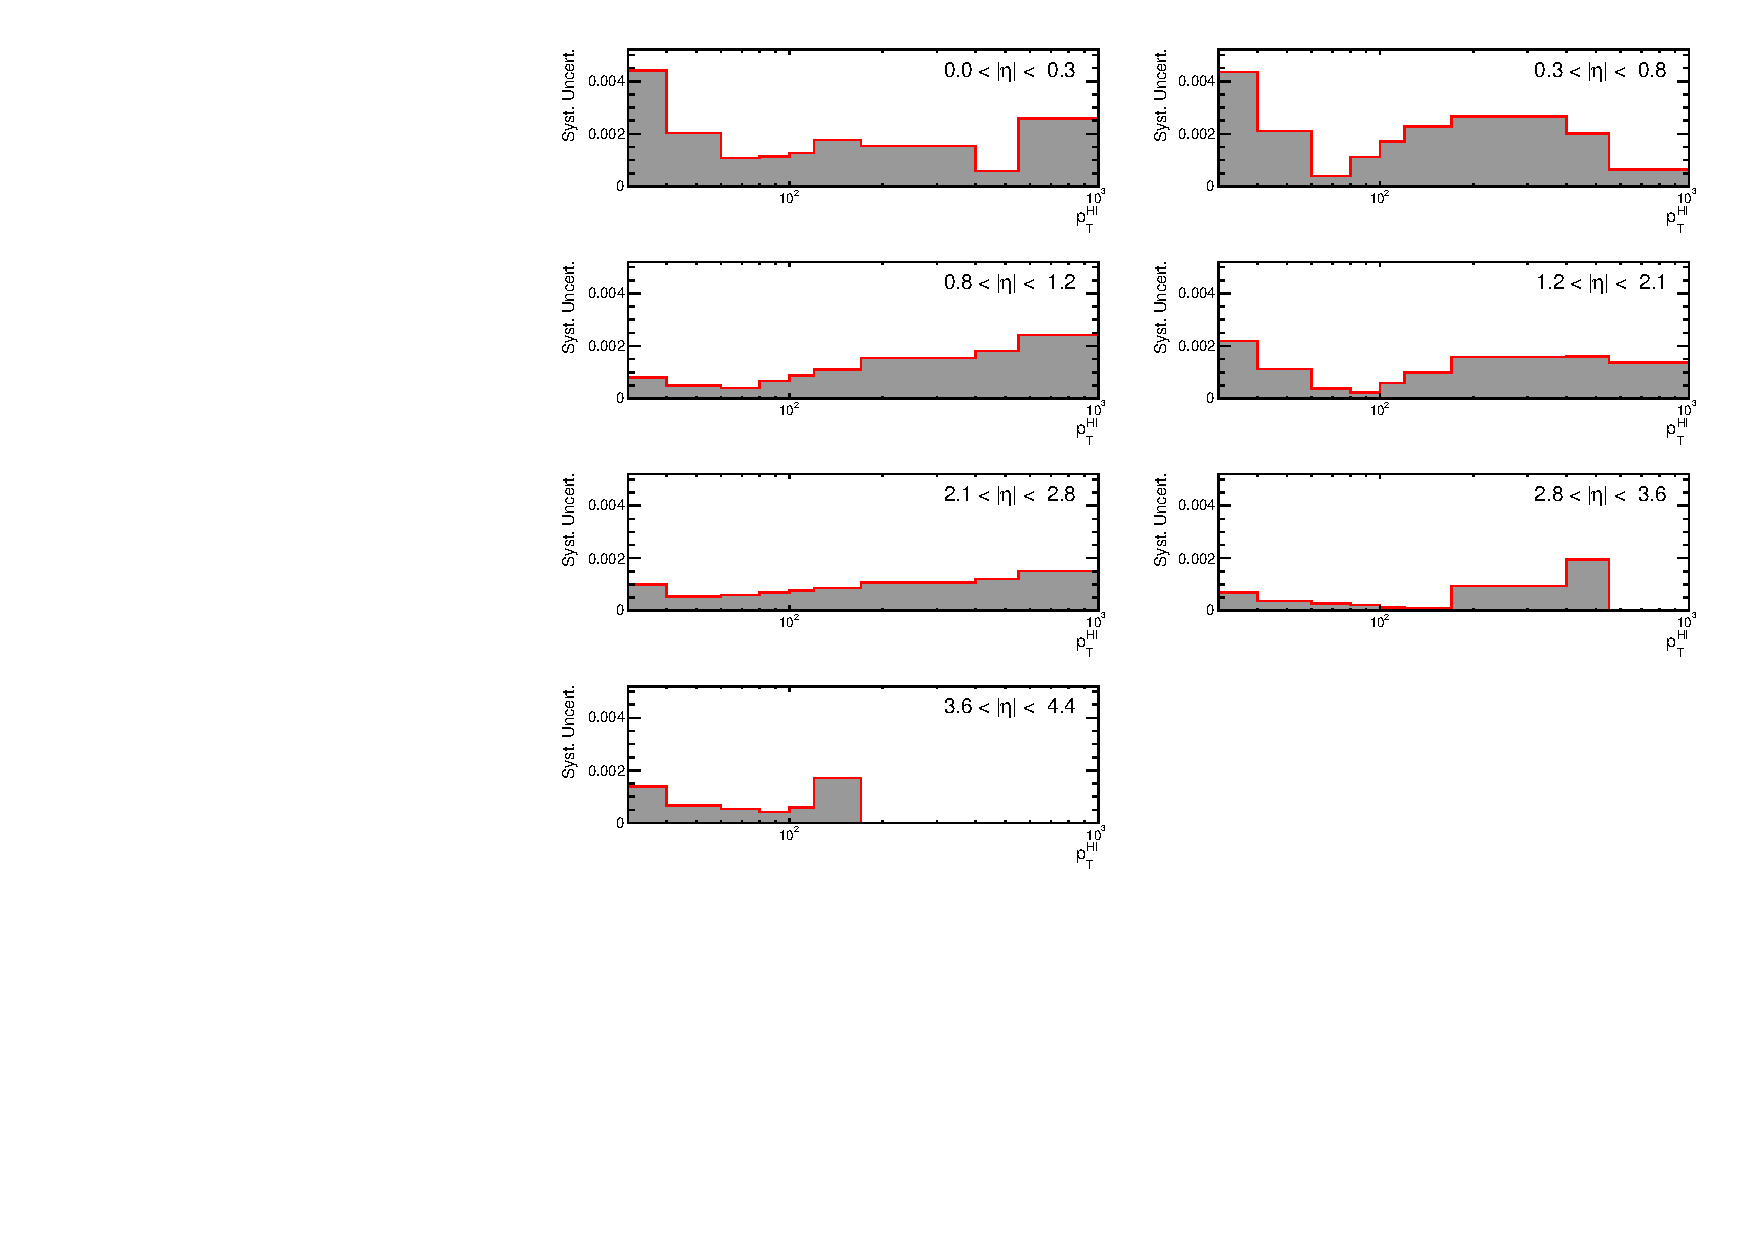
\includegraphics[width=1.0\textwidth]{figures/qualification/sys_uncert} }}%
	\caption{The systematic uncertainty, equal to maximum difference between the nominal fit and the fits from varying the parameters (as summarized in Table~\ref{table:systematics_param}).  }
	\label{fig:sys_uncert}%
\end{figure}


%---
\subsection{Uncertainties on HI JER}
\label{sec:qual_jeruncertainties}
%---
The uncertainties on the heavy ion jet energy resolution ($\dsigma_\hi$ ) can be shown to be given by: 
\begin{align}
\dsigma_{\hi} = \frac{\delta R_{\hi}}{2 \sigma_{\hi}}
\end{align} 
where $R_\hi = \sigma_\hi^2$. We also can also derive (see \ref{sec:appendix_hijerDerivation} for derivation):
\begin{align}
\delta^2 R_\hi &= \lambda^4 \delta^2 R_\emt + \delta^2 B \\
\delta R_\emt  &= 2 \sigma_\emt \dsigma_\emt \\
\lambda &= \frac{\mathrm{Cov}(\Delta \pT^\emt | _\mathrm{noGSC}, \Delta \pT^\hi)}{\mathrm{Cov}(\Delta \pT^\emt | _\mathrm{GSC}, \Delta \pT^\hi)} \label{eq:lambda} \\ 
\delta B &= \sigma(\pT^\hi/\pt^\emt)_\mathrm{data} - \sigma(\pT^\hi/\pt^\emt)_\mathrm{MC} 
\end{align} 

$\sigma_{\emt}$ and $\dsigma_{\emt}$ were evaluated using the JER tool \cite{JERTool}, whereas $\sigma_\hi$ was measured in the data (shown in Fig~\ref{fig:emtopo_jer}. $\lambda$ was determined using $\Delta\pT^\emt = \pT^\emt - \pT^\tru$ and $\Delta\pT^\hi =\pT^\hi - \pT^\tru$ evaluated with and without the GSC calibration. 

Fluctuations in $\sigma_\emt$ and $\sigma_\hi$ were removed by fitting to the form
\begin{align}
a+(b/\pT)+(c/\pT)^2
\label{fit:jer_fit}
\end{align}
These are shown in Fig.~\ref{fig:fitted_jer}. The $\Delta\pT^\emt$ vs. $\Delta\pT^\hi$ for with and without the GSC can be seen in Fig.~\ref{fig:deltapT_w_gsc} and Fig.~\ref{fig:deltapT_no_gsc} respectively. The $\lambda$ distribution can be seen in Fig.~\ref{fig:lambda}. A comparison between $\delta\sigma_\emt$ and $\delta\sigma_\hi$ can be seen in Fig.~\ref{fig:meth2_jer_uncert}. The ratio $\delta\sigma_\emt / \delta\sigma_\hi$ can be expressed as below:
\begin{align}
\frac{\delta\sigma_\hi}{\delta\sigma_\emt} = \frac{\delta R_\hi}{\delta R_\emt} \frac{\sigma_\emt}{\sigma_\hi}
\end{align}
This factorization (plotted in Fit.~\ref{fig:meth2_ratios}) showed that the large differences between $\delta\sigma_\emt$ and $\delta\sigma_\hi$ were coming from the differences in the uncertainties, as opposed to differences in the actual resolutions themselves. The same quantity, $\delta\sigma_\emt / \delta\sigma_\hi$, as calculated in Run I is shown in Fig.~\ref{fig:run1_jer_uncert} \cite{xcalib_run1}.


\begin{figure}
	\centering
	\subfloat{{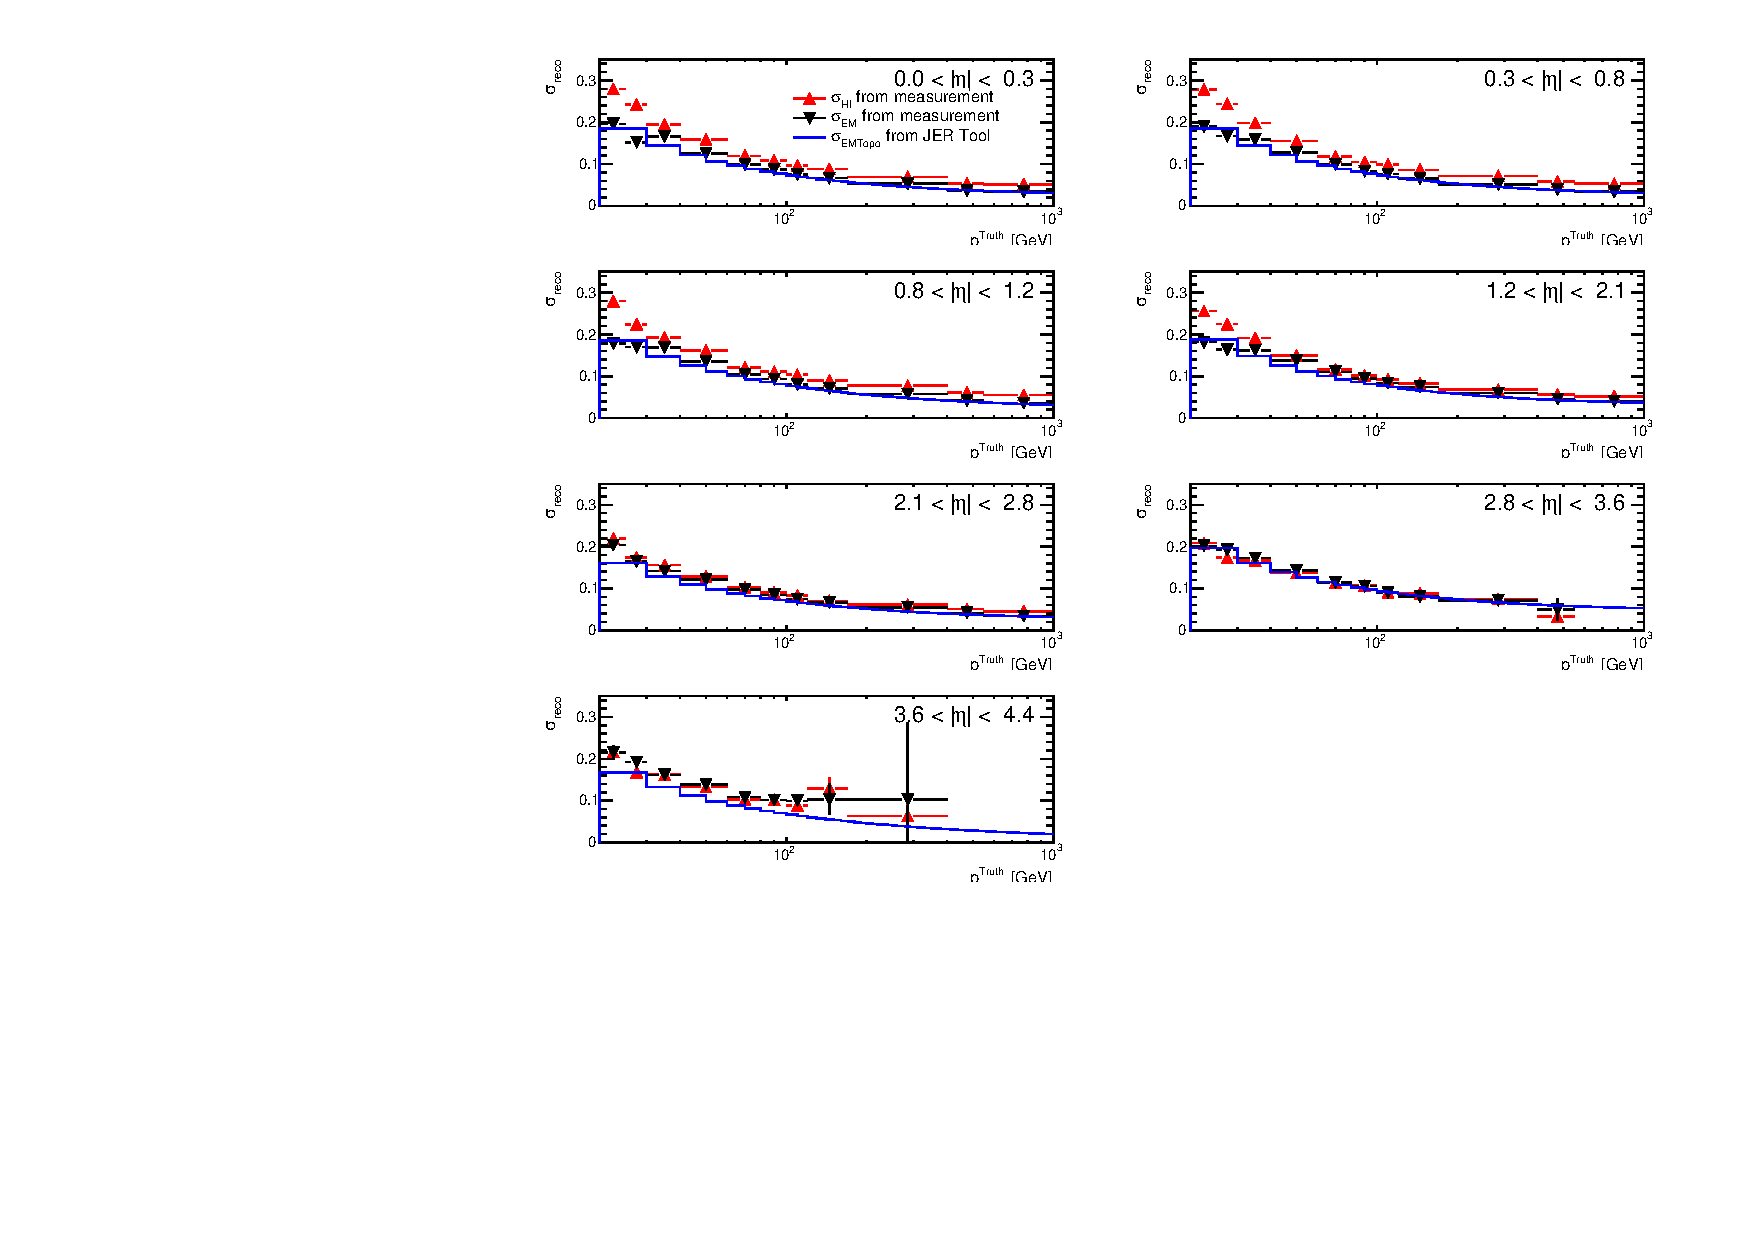
\includegraphics[height=0.5\textwidth]{figures/qualification/emtopo_jer} }}%
	\caption{A comparison of the JER of EMTopo and HI jets from the datasets, as well as from the JER Tool. }
	\label{fig:emtopo_jer}%

	\centering
	\subfloat{{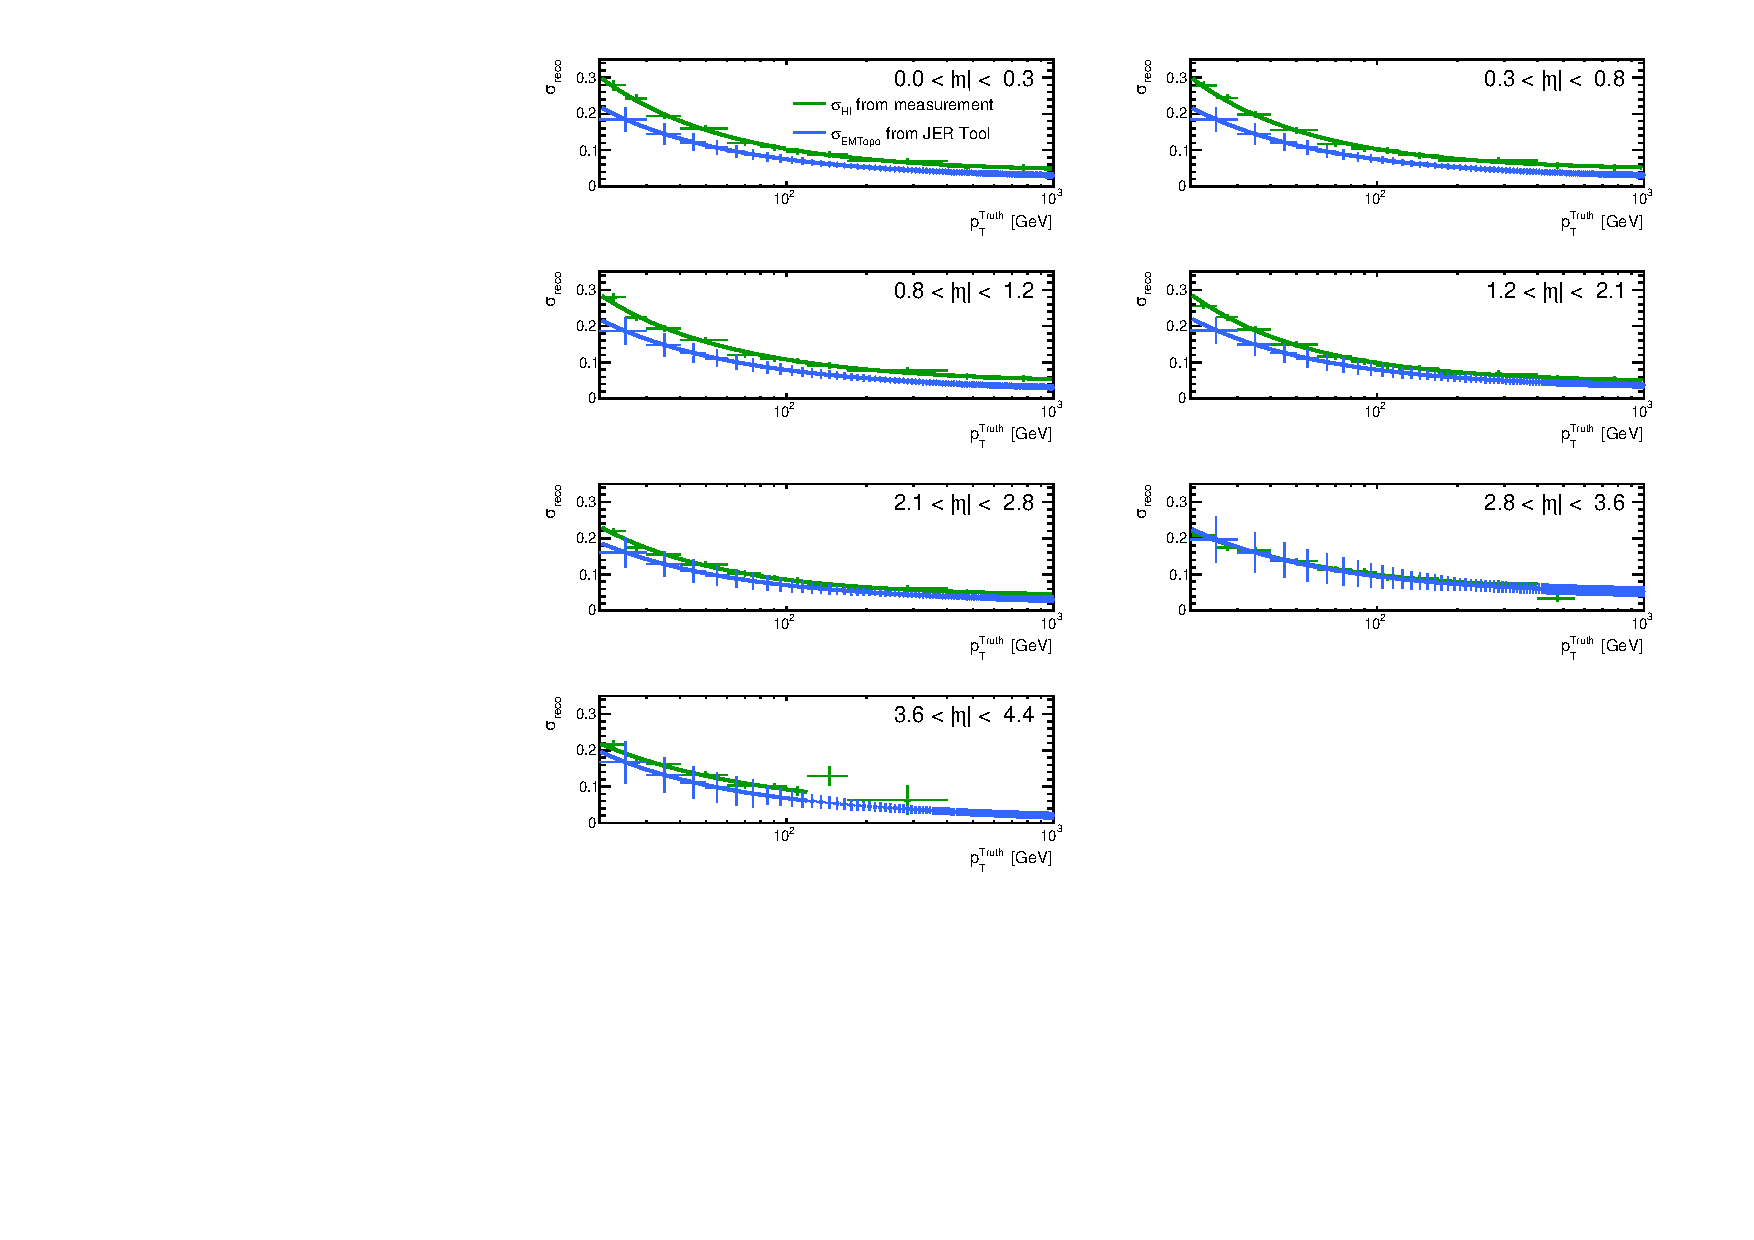
\includegraphics[height=0.5\textwidth]{figures/qualification/fitted_jer} }}%
	\caption{The JER for $\hi$ and $\emt$ jets fit to Eq.~\ref{fit:jer_fit}}
	\label{fig:fitted_jer}%
\end{figure}

\begin{figure}
	\centering
	\subfloat{{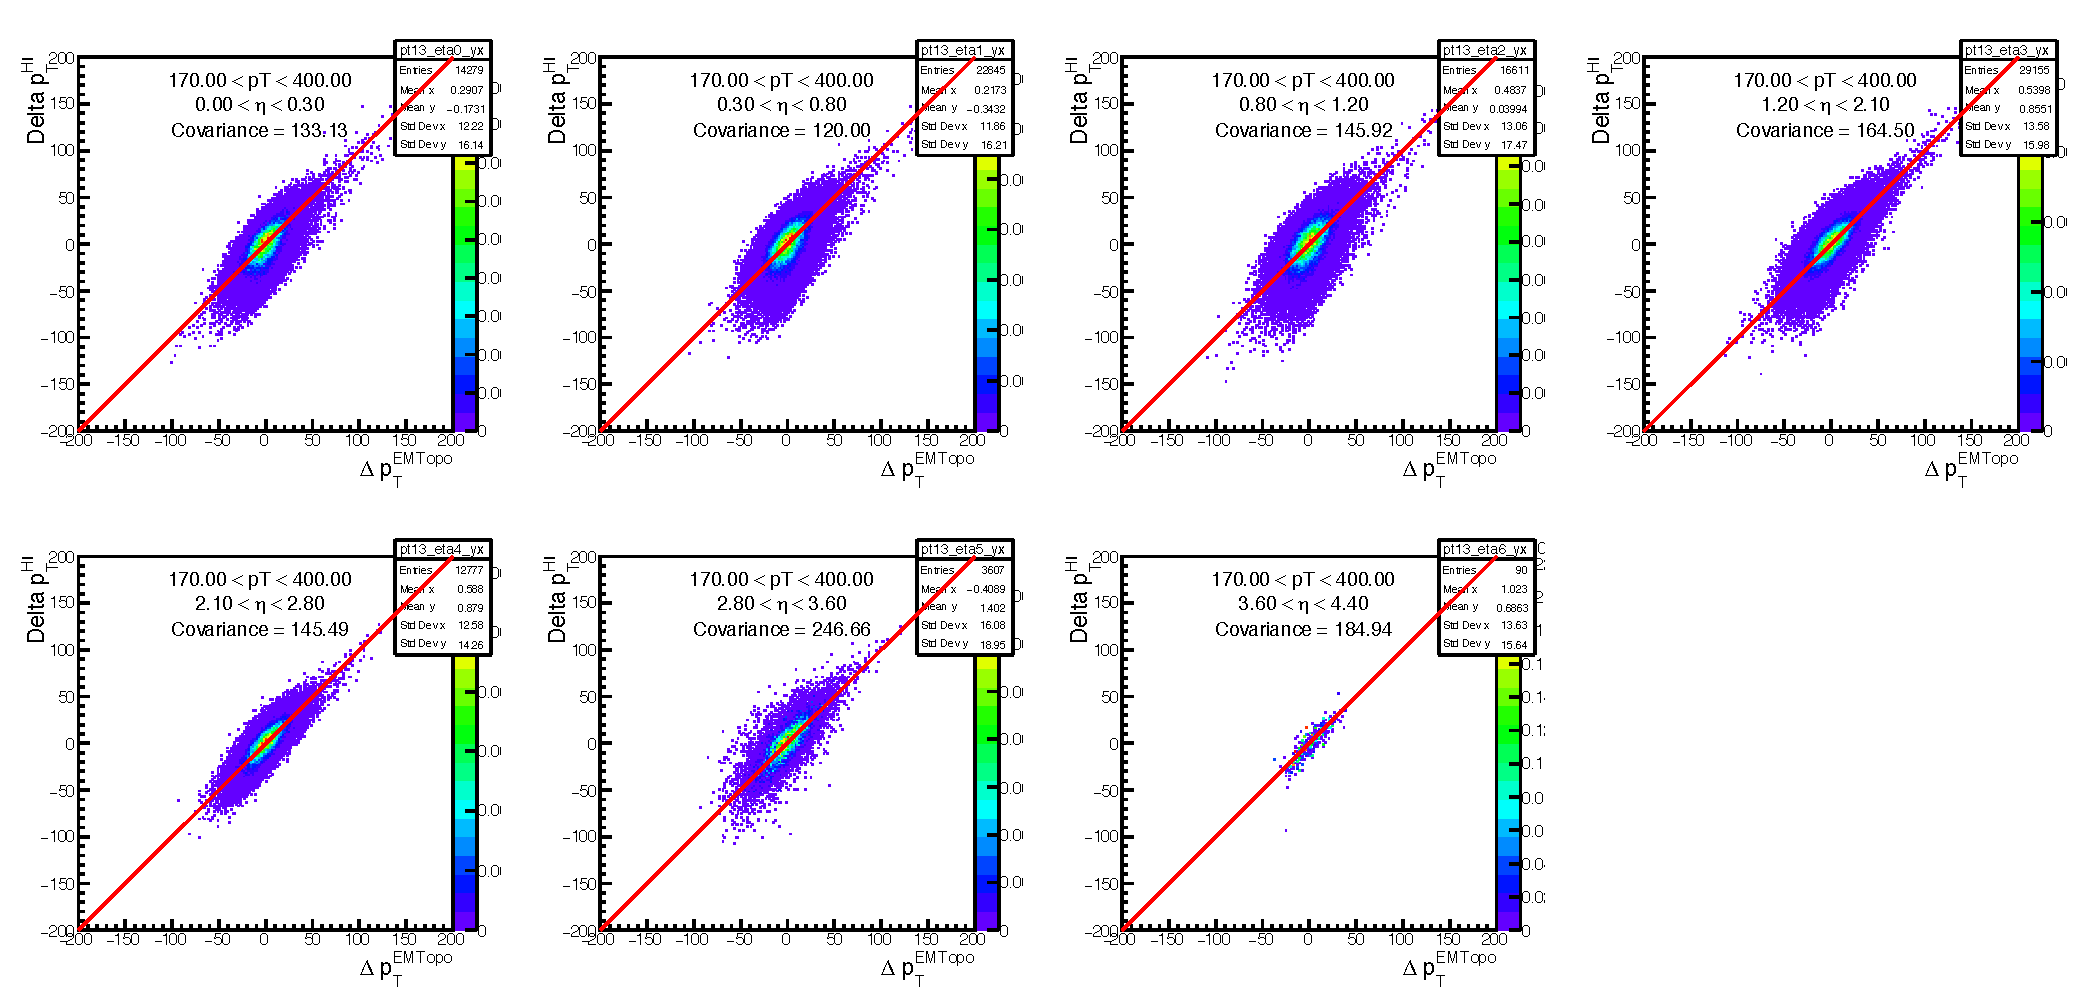
\includegraphics[height=0.5\textwidth]{figures/qualification/deltapT_w_gsc} }}%
	\caption{The $\Delta\pT^\emt$ vs. $\Delta\pT^\hi$ distribution in all $\eta$ bins, for $ 170 < \pT^\tru < 400$ GeV, with the GSC calibration applied to the $\emt$ jets. }
	\label{fig:deltapT_w_gsc}%
	
	\centering
	\subfloat{{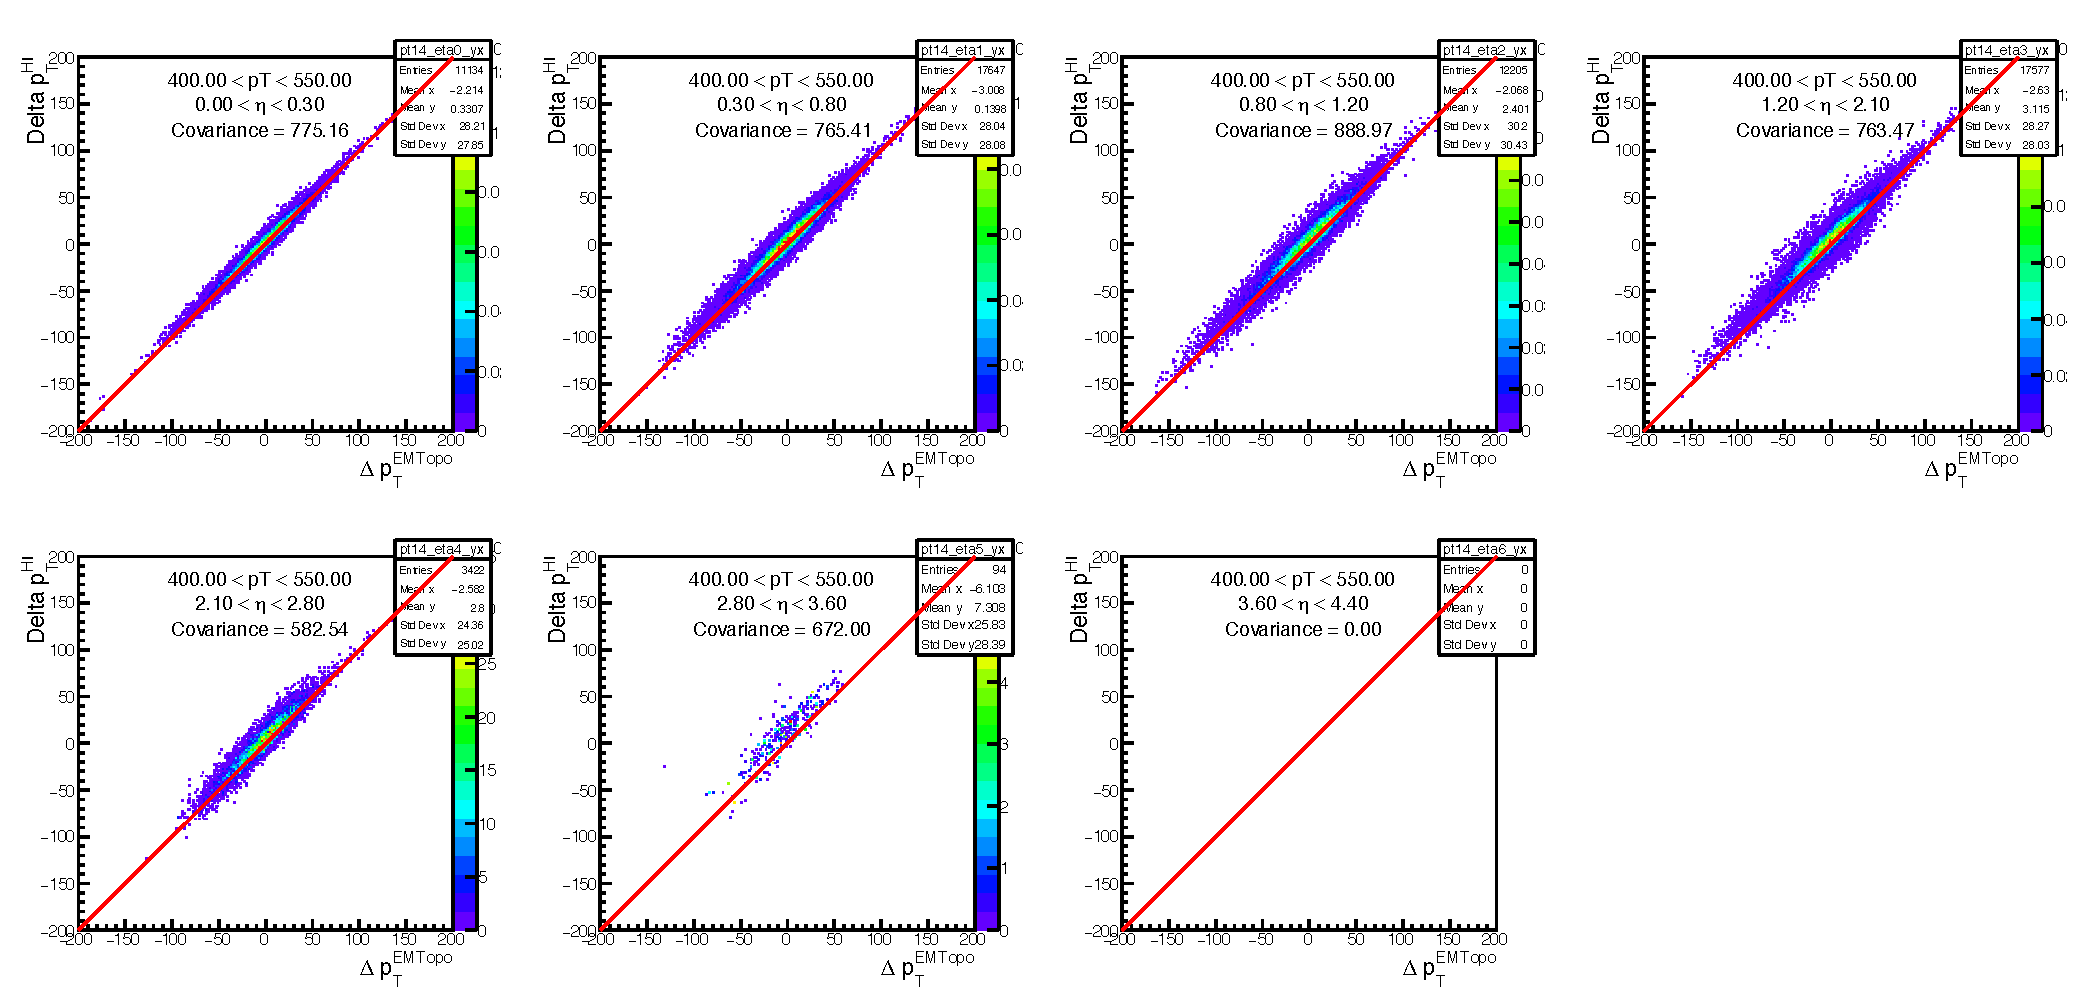
\includegraphics[height=0.5\textwidth]{figures/qualification/deltapT_no_gsc} }}%
	\caption{The $\Delta\pT^\emt$ vs. $\Delta\pT^\hi$ distribution in all $\eta$ for $ 170 < \pT^\tru < 400$ GeV, with no GSC calibration applied to the $\emt$ jets. }
	\label{fig:deltapT_no_gsc}%
\end{figure}


\begin{figure}
	\centering
	\subfloat{{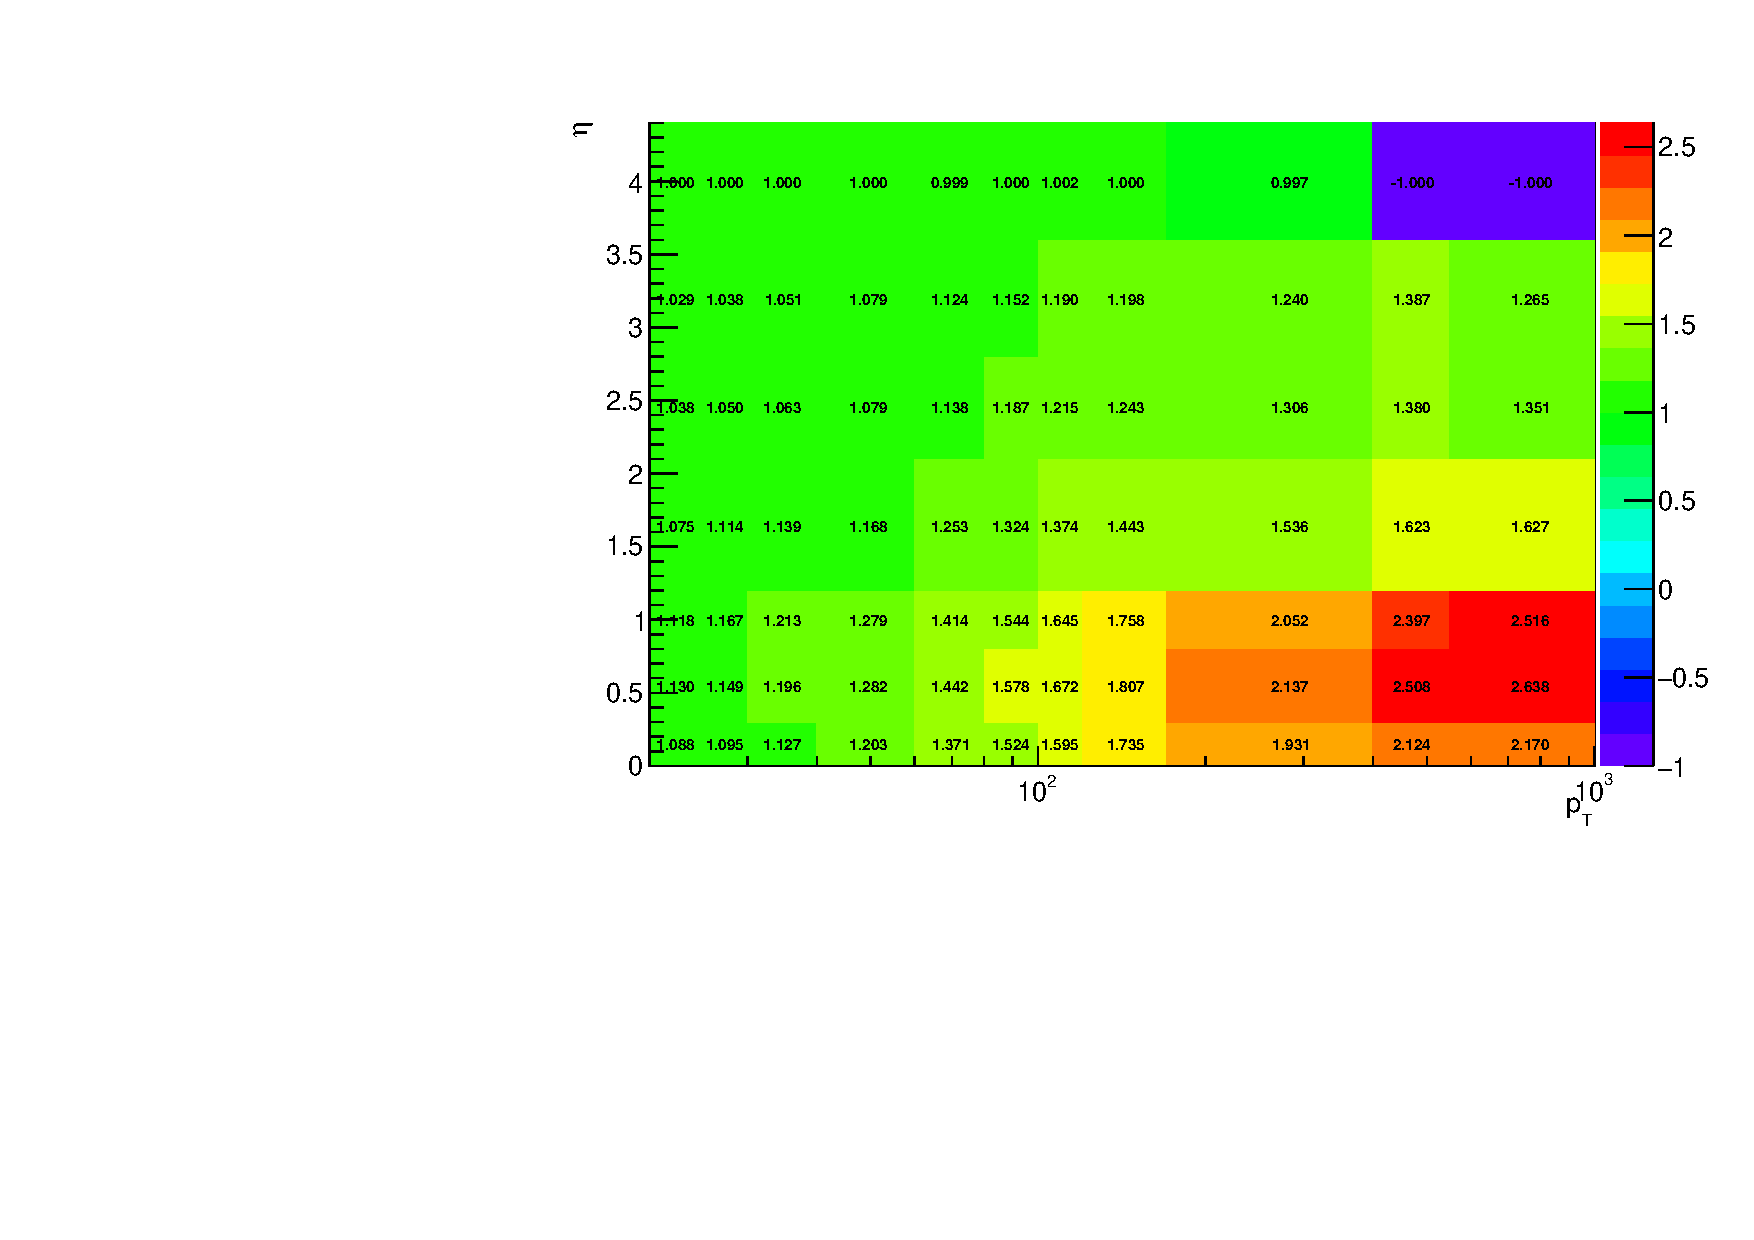
\includegraphics[width=0.8\textwidth]{figures/qualification/lambda} }}%
	\caption{The distribution of $\lambda$ as calculated in Eq.~\ref{eq:lambda} in various bins of $\pt$ and $\eta$.}
	\label{fig:lambda}%
\end{figure}

\begin{figure}
	\centering
	\subfloat{{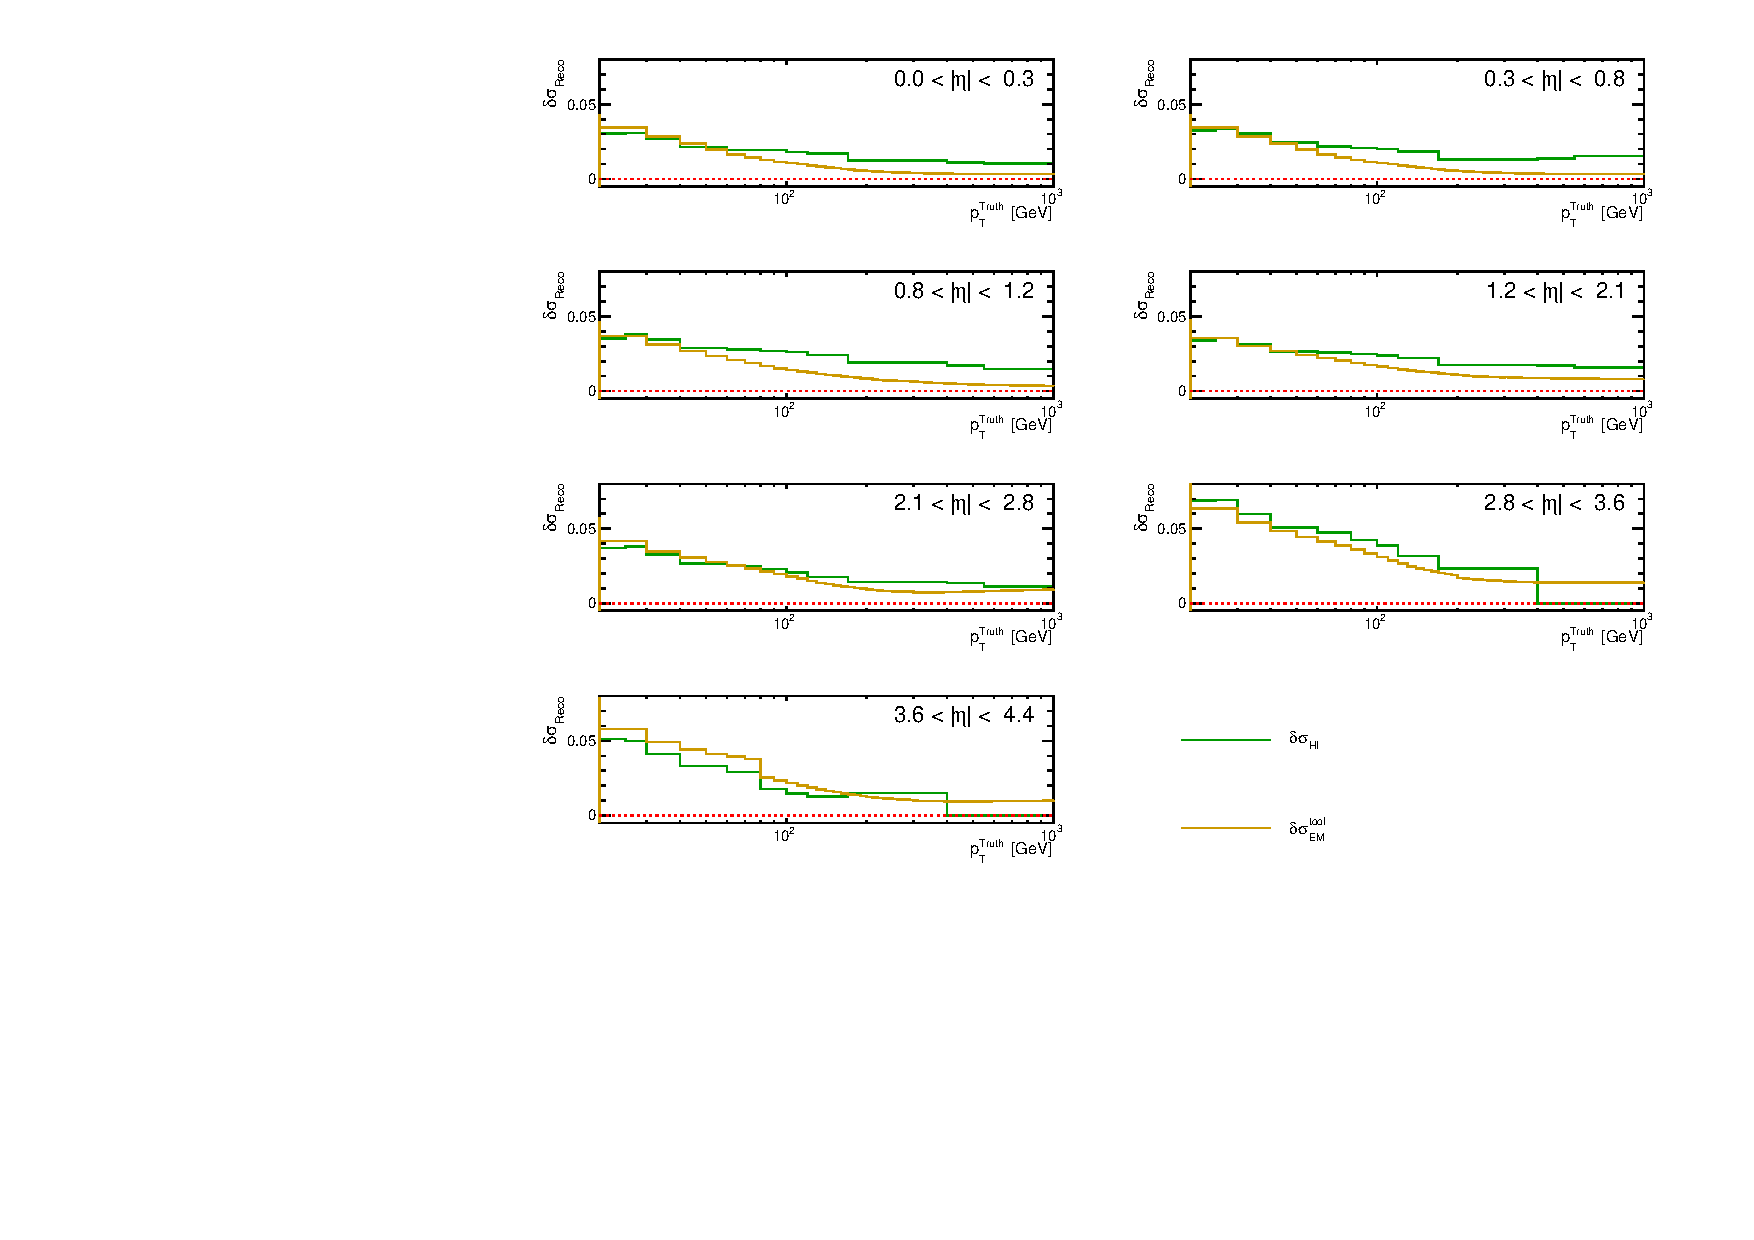
\includegraphics[width=0.8\textwidth]{figures/qualification/meth2_jer_uncert} }}%
	\caption{A comparison between $\delta\sigma_\emt$ and $\delta\sigma_\hi$ in various $\eta$ bins}
	\label{fig:meth2_jer_uncert}%
\end{figure}

\begin{figure}
	\centering
	\subfloat{{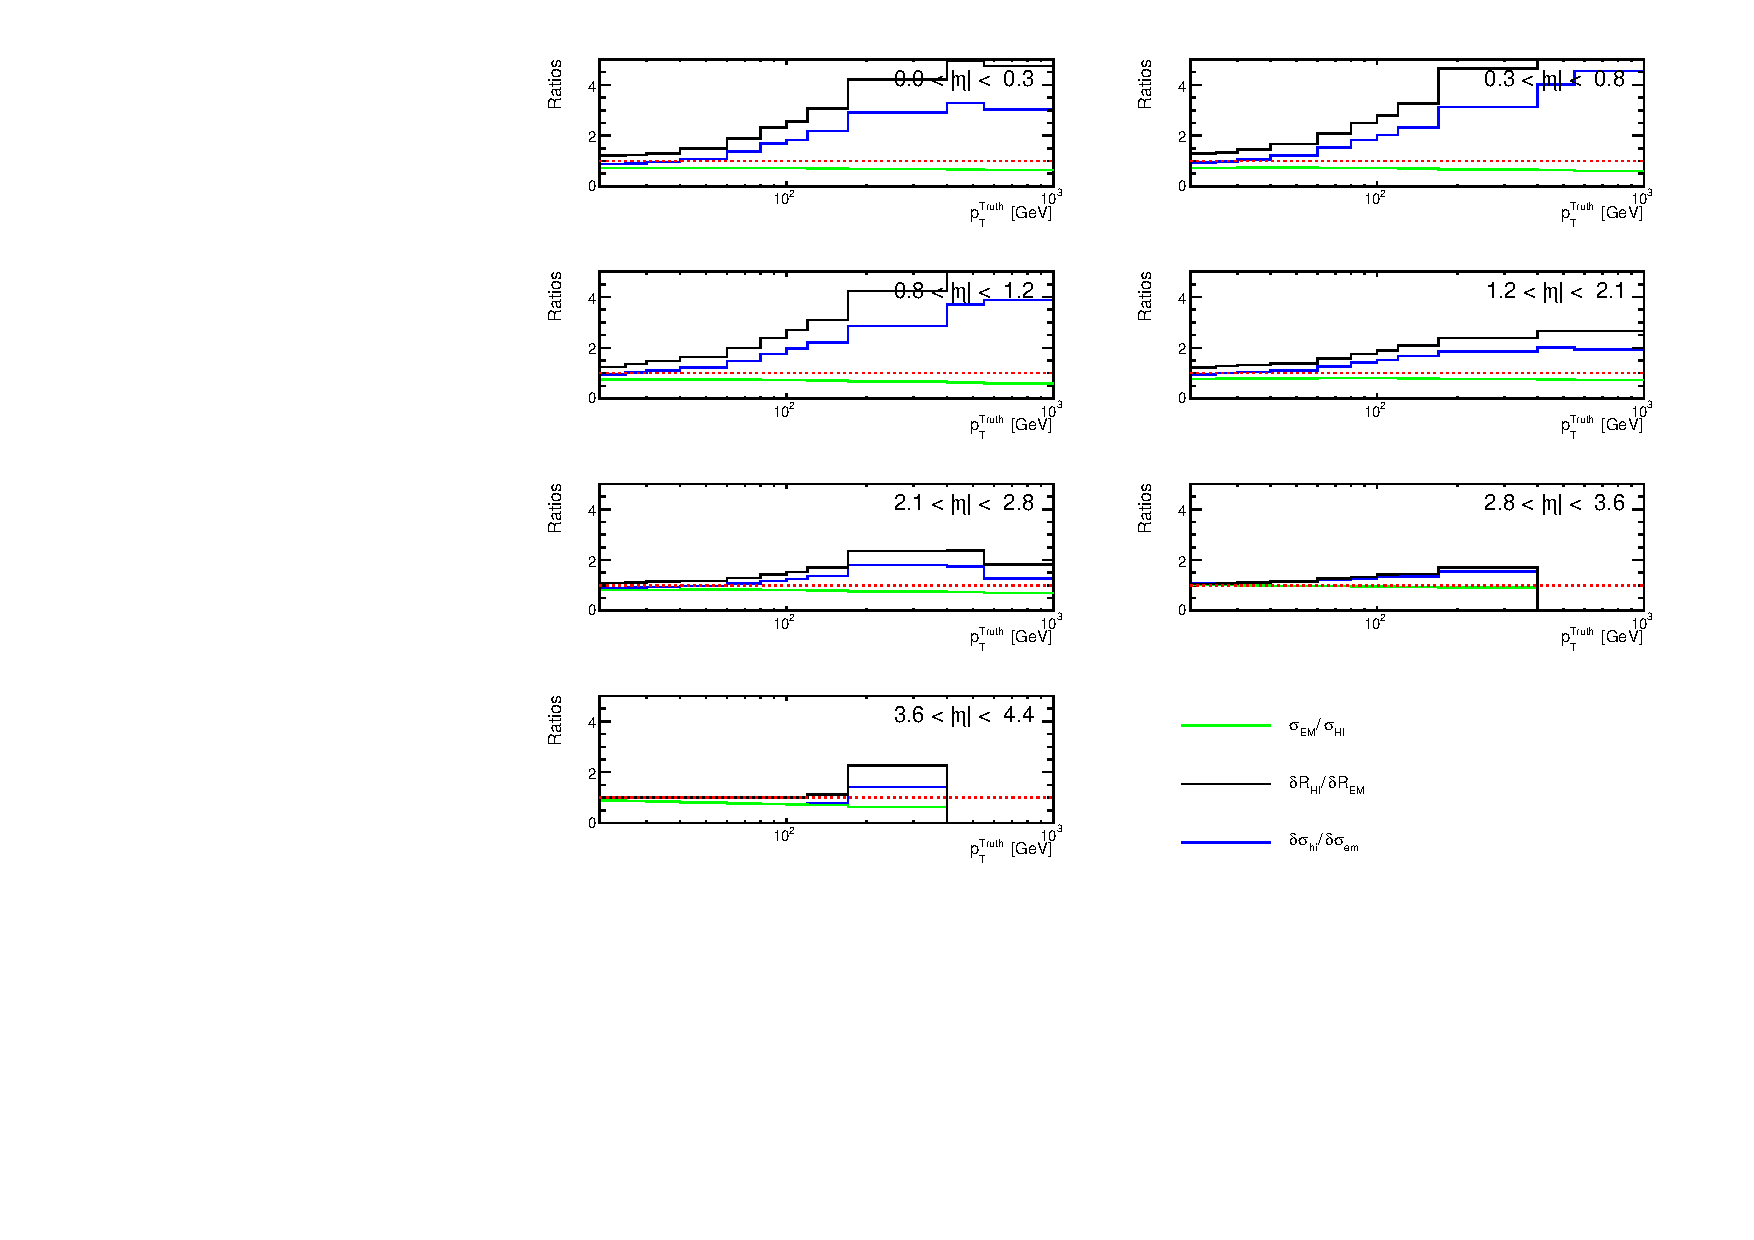
\includegraphics[width=0.8\textwidth]{figures/qualification/meth2_ratios} }}%
	\caption{Factorizing the ratio $\delta\sigma_\emt / \delta\sigma_\hi$ shows that the dominant effect is from the uncertainties themselves (as opposed to a difference in the resolutions)}
	\label{fig:meth2_ratios}%
\end{figure}

\begin{figure}
	\centering
	\subfloat{{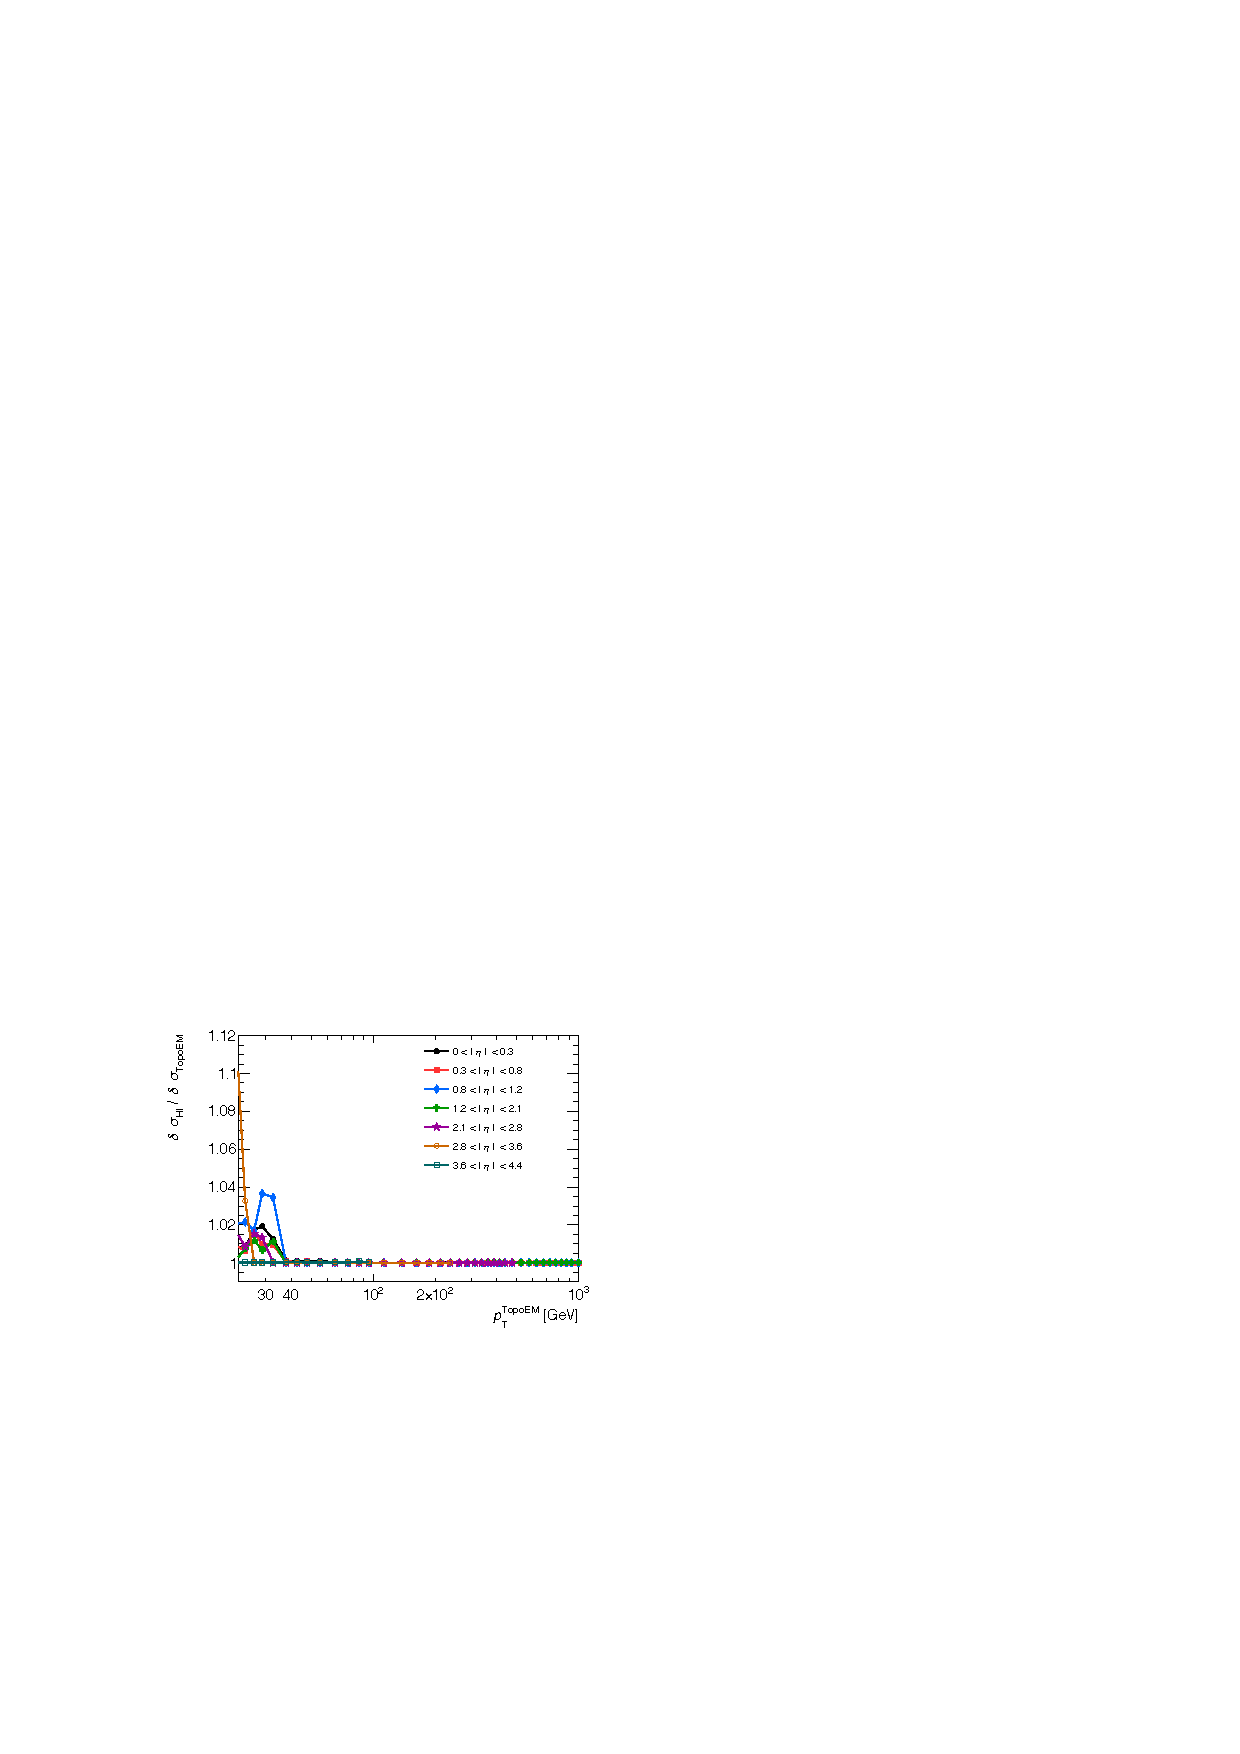
\includegraphics[width=0.8\textwidth]{figures/qualification/run1_jer_uncert} }}%
	\caption{The ratio $\delta\sigma_\emt / \delta\sigma_\hi$ as evaluated in Run I \cite{xcalib_run1}}
	\label{fig:run1_jer_uncert}%
\end{figure}


%-------------------------------------------------------------------------------
\section{Qualification Task Conclusion}
\label{sec:qual_result}
%-------------------------------------------------------------------------------
The cross calibration factors, along with its systematic and statistical uncertainties were derived in different $\eta$ regions, as a function of $\pT^{\hi}$, and are shown in Fig.~\ref{fig:factors_w_uncertainties}. The factors themselves are the level of ~1\%, and do not show much variation with $\pT$.  Furthermore, the uncertainties are primarily statistical in nature. 

\begin{figure}
	\centering
	\subfloat{{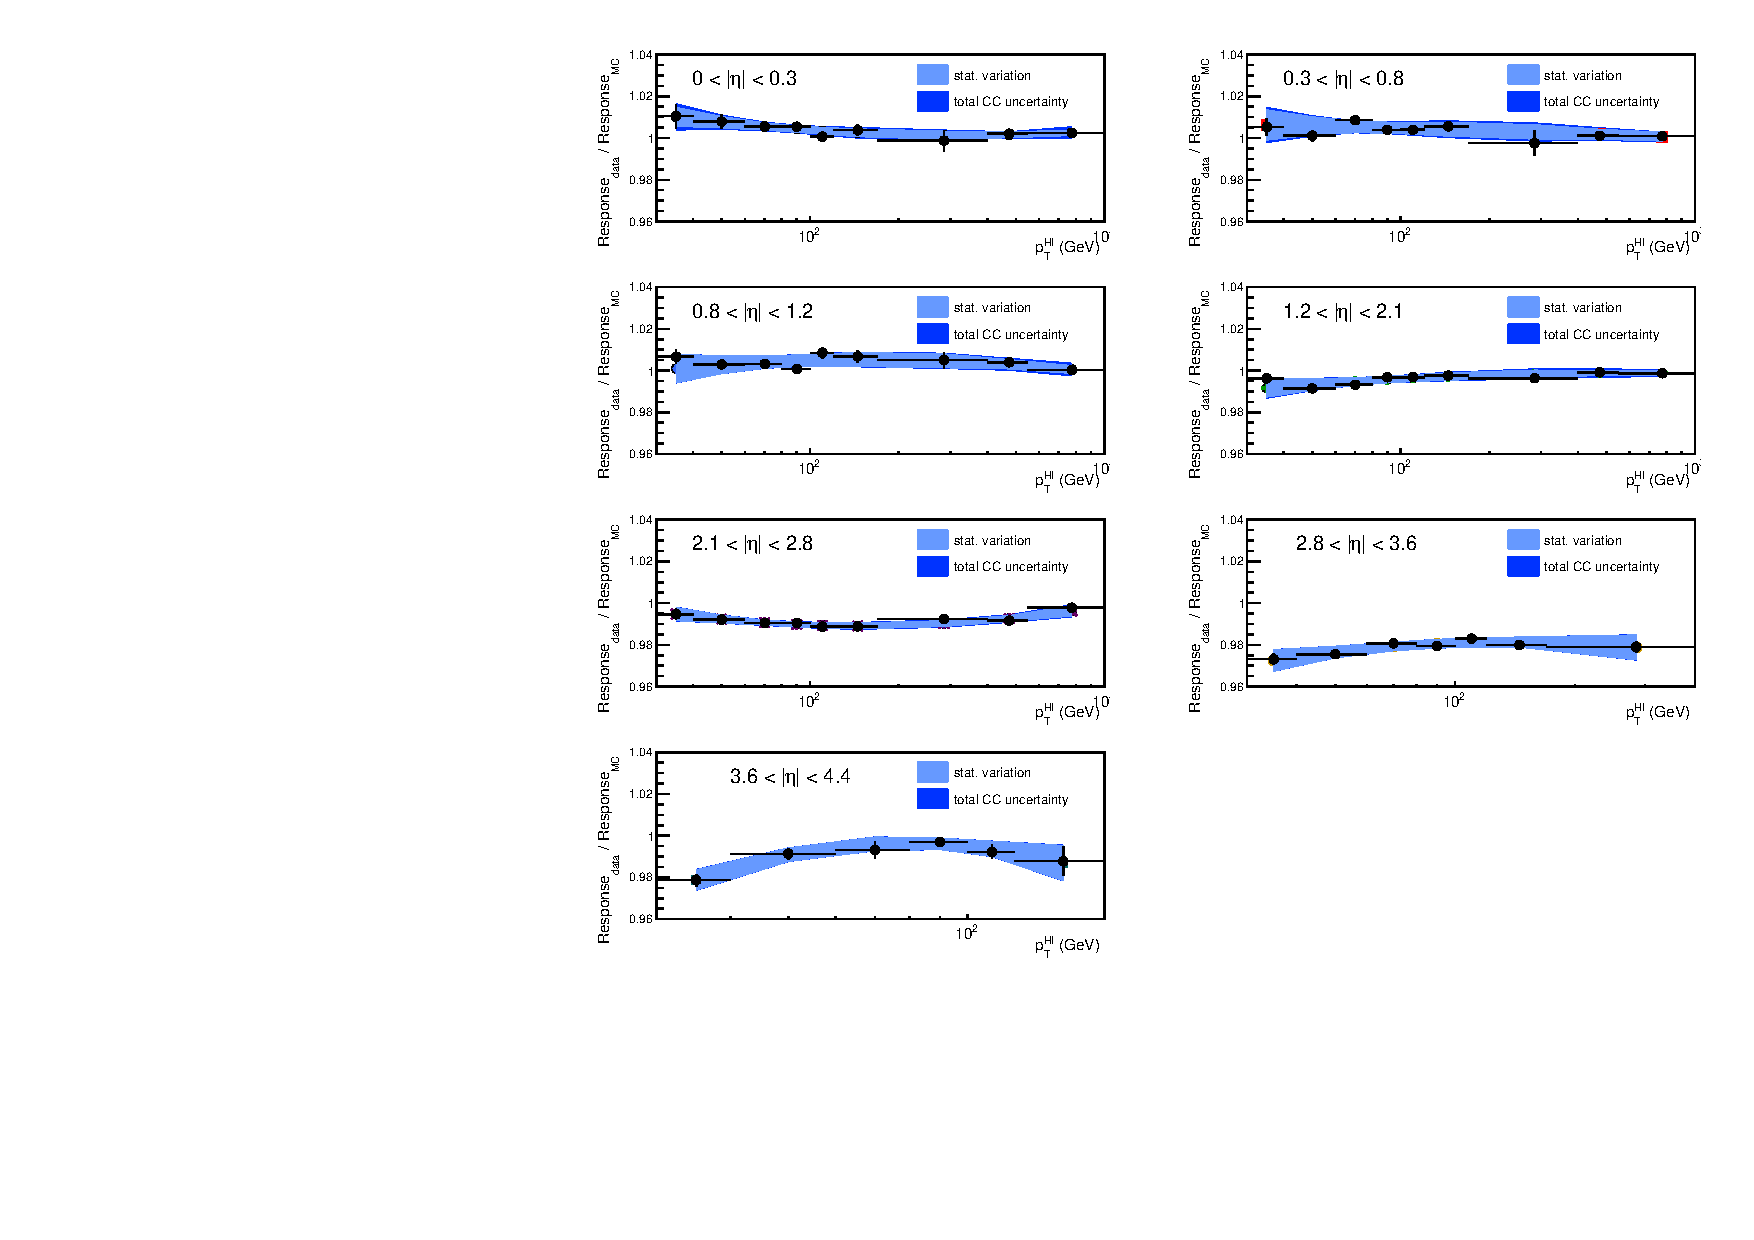
\includegraphics[width=1.0\textwidth]{figures/qualification/factors_w_uncertainties} }}%
	\caption{The cross calibration factors in different $\eta$ regions, as a function of $\pT^{\hi}$, along with their uncertainties.}
	\label{fig:factors_w_uncertainties}%
\end{figure}

 A $\pT$ dependent uncertainty on the HI JER was also derived, and can be seen in Fig.~\ref{fig:meth2_jer_uncert}.


%
%%%%%%%%%%%%%%%%%%%%%%%%%%%%%%%%%%%%%%%%%%%%%%%%%%%%%%%%%%%%%%%%%%%%%%%
%\subsection{Cross Calibration and its uncertainties}
%The hadronic shower (jet) has both electromagnetic and non-electromagnetic components that interact with the calorimeter material differently. Thus the energy response of the calorimeter for these components is different (this is called a non-compensating calorimeter \cite{calorimetry_book}), and hence, calibrations are required to correct the reconstructed jet kinematics. These take into account features of the detector, the reconstruction algorithm, and jet fragmentation. The final corrections come from data driven (\insitu) methods like \pt\ balance studies (comparing the \pt\ of a jet and any other object like another jet, Z, or $\gamma$). Heavy ion collisions however, have the limitation that simple \pt\ balance studies are non-trivial because of jet quenching effects. Another limitation is the lack of high statistics for reference objects like $Z$'s and photons. The way to get around this is to derive a \textit{cross}-calibration, based on comparing jets in \pp\ collisions, as reconstructed by the heavy ion and \pp\ jet reconstruction algorithms. The HI jets can then be scaled with factors given by the ratio of $\langle \pt ^\hi / \pt^\emt \rangle$ in data and MC.
%
%The statistical uncertainties on the cross calibration factors come from the fits to the ratio of the relative response in data and MC, whereas the systematics come from changing the parameters of the study (these were evaluated as the maximum absolute difference between the nominal fit and any other iteration). The cross calibration factors for $0.8 < |\eta| < 1.2$, along with their uncertainties are shown on Fig.~\ref{fig:factors_w_uncertainties}. These are at the level of about 1\% and do not show strong variation with \pt. 
%\begin{figure}[htbp!]
%	\centering
%	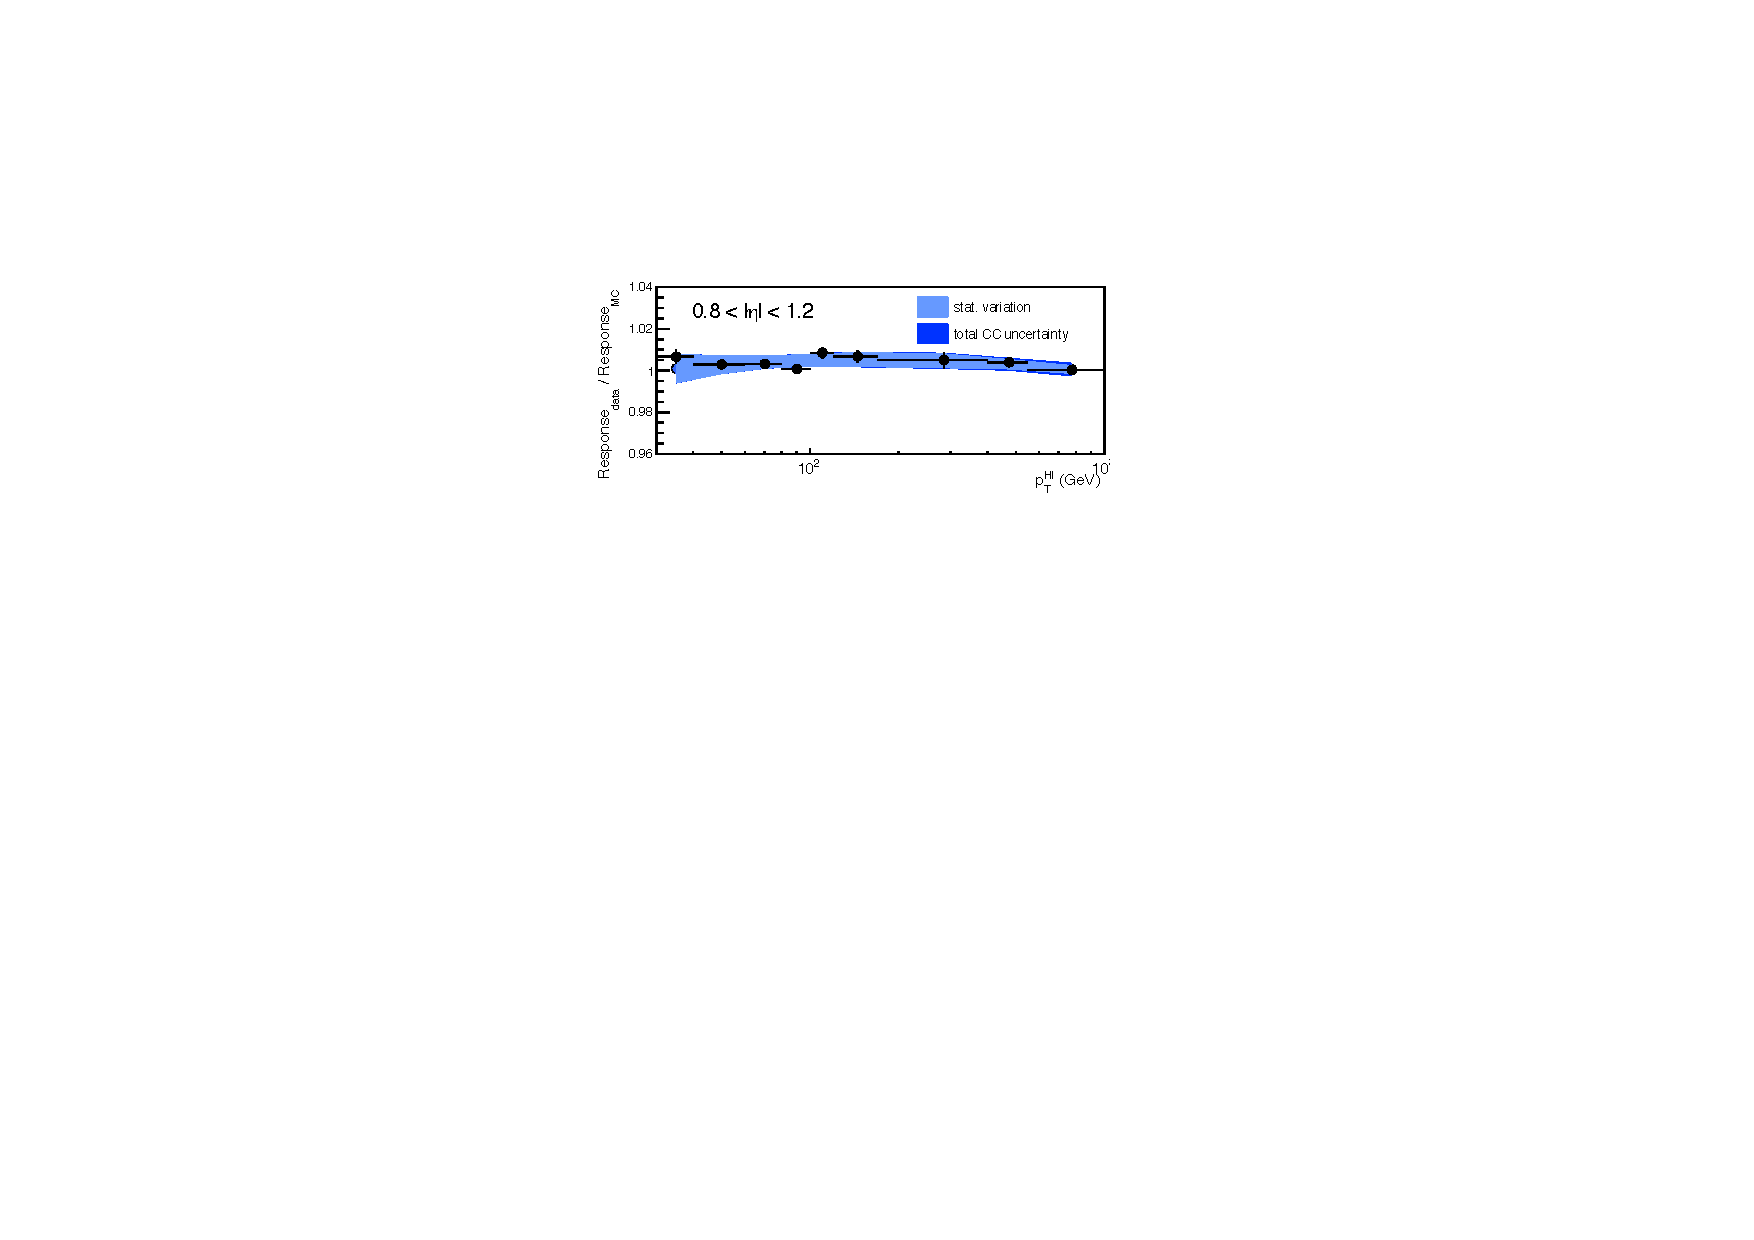
\includegraphics[width=0.5\textwidth]{figures/qualification/factors_w_uncertainties_2}
%	\caption{The cross calibration factors for $0.8 < |\eta| < 1.2$, as a function of $\textit{p}_{\text{T}}^{\text{HI}}$, along with their uncertainties.}
%	\label{fig:factors_w_uncertainties}%
%\end{figure}
%
%
%The cross-calibration procedure further allows applying the baseline jet energy scale/resolution uncertainties from the EMTopo jets, to the HI jets (along with the uncertainties of the cross-calibration procedure itself) \cite{xcalib_run1}. 
%
%
%\subsection{Heavy Ion Jet Energy Resolution Uncertainties}
%The uncertainty on the heavy ion jet energy resolution can be shown to be given by:
%
%\begin{equation}
%\delta \sigma_{\text{HI}} = \delta \sigma_{\text{EMTopo}} \sqrt{\left(1 + \frac{A}{\sigma_{\text{HI}}^2}\right)\left(1 + \left[\frac{\delta A}{2 \sigma_{\text{EMTopo}} \delta \sigma_{\text{EMTopo}}}\right)\right]^2} 
%\end{equation}
%where $\delta A ^2 = (2 s _{\text{HI}} \delta s _{\text{HI}})^2  + (2 s _{\text{EMTopo}} \delta s _{\text{EMTopo}})^2$ and $s^2_{\text{EMTopo/HI}}$ is the uncorrelated component between the errors in the jet \pt\, as reconstructed by two different algorithms applied to the same data \cite{xcalib_run1}. This result however, neglects that the uncertainty in the EMTopo jet energy resolution can be correlated with the systematic uncertainty on $A$. Accounting for this correlation, it can be shown that the uncertainty on the heavy ion jet energy resolution can be given by:
%\begin{equation}
%\dsigma_{{\text{HI}}} = \frac{\delta R_{{\text{HI}}}}{2 \sigma_{{\text{HI}}}}
%\end{equation}
%where
%\begin{align}
%R_{\text{HI}} &= \sigma_{\text{HI}}^2 \\
%\delta^2 R_{\text{HI}} &= \lambda^4 \delta^2 R_\emt + \delta^2 B \\
%\delta R_\emt  &= 2 \sigma_\emt \dsigma_\emt
%\end{align}
%Here, $\lambda$ accounts for the correlation between the HI and EMTopo jets, and $B$ is a estimate of the difference in the relative resolution between HI and EMTopo jets, as measured in data and MC.
%
%A comparison between $\delta\sigma_\emt$ and $\delta\sigma_{\text{HI}}$ can be seen in Fig.~\ref{fig:hi_jer_uncert}.
%
%
%\begin{figure}[htbp!]
%	\centering
%	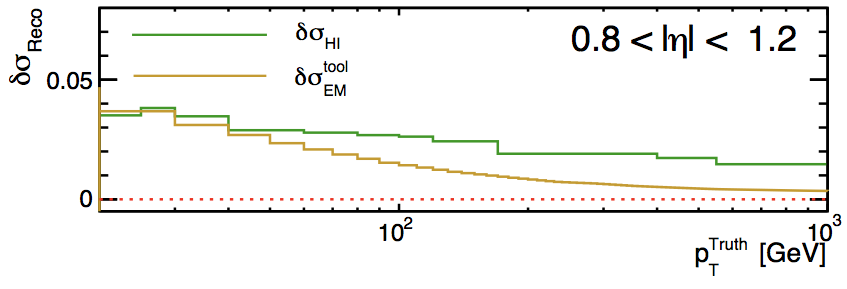
\includegraphics[width=0.7\textwidth]{figures/qualification/uncert_2} %
%	\caption{The comparison between $\delta\sigma_\emt$ and $\delta\sigma_{\text{HI}}$ for $0.8 < |\eta| < 1.2$.}	
%	\label{fig:hi_jer_uncert}%
%\end{figure}
%
%\section{Fragmentation functions}
%I am currently working on deriving the fragmentation functions for jets in \PbPb\ collisions at \sqrtsnn\ = 5.02 TeV, and comparing them to \pp\ fragmentation functions at the same collision energy \cite{ATLAS-CONF-2017-005}. These measurements provide information about the momentum fraction distribution of charged particles inside jets.
%
%The fragmentation functions can be defined in terms of the longitudinal momentum fraction ($z$) of the particle relative to a jet as follows
%
%\begin{align}
%D(z) \equiv \frac{1}{N_{\text{jet}}} \frac{dN_{\text{ch}}}{dz}, \quad \quad
%z \equiv \frac{\pttrk}{\pTjet} \cos\Delta R
%\end{align}
%where $N_{\text{ch}}$ is the number of charged particles, and $N_{\text{jet}}$ is the number of jets being studied. The comparison of $D(z)$ between \PbPb\ and \pp\ collisions helps in understanding the strength and mechanism of medium induced jet quenching, and can be quantified by $R_{D(z)} \equiv {D(z)_{\text{PbPb}}}/{D(z)_{\text{pp}}}$
%
%Our results, shown in Fig.~\ref{fig:ff_502}, indicate that jets in \PbPb\ collisions have an enhancement of particles for $z > 0.2$, and a depletion for lower $z$ values, with the modification decreasing with decreasing centrality. This is qualitatively consistent with previous measurements done by ATLAS and CMS at 2.76 TeV \cite{Aaboud:2017bzv, Aad2014320, Chatrchyan:2014ava}. 
%
%
%\begin{figure}[htbp!]
%	\centering
%	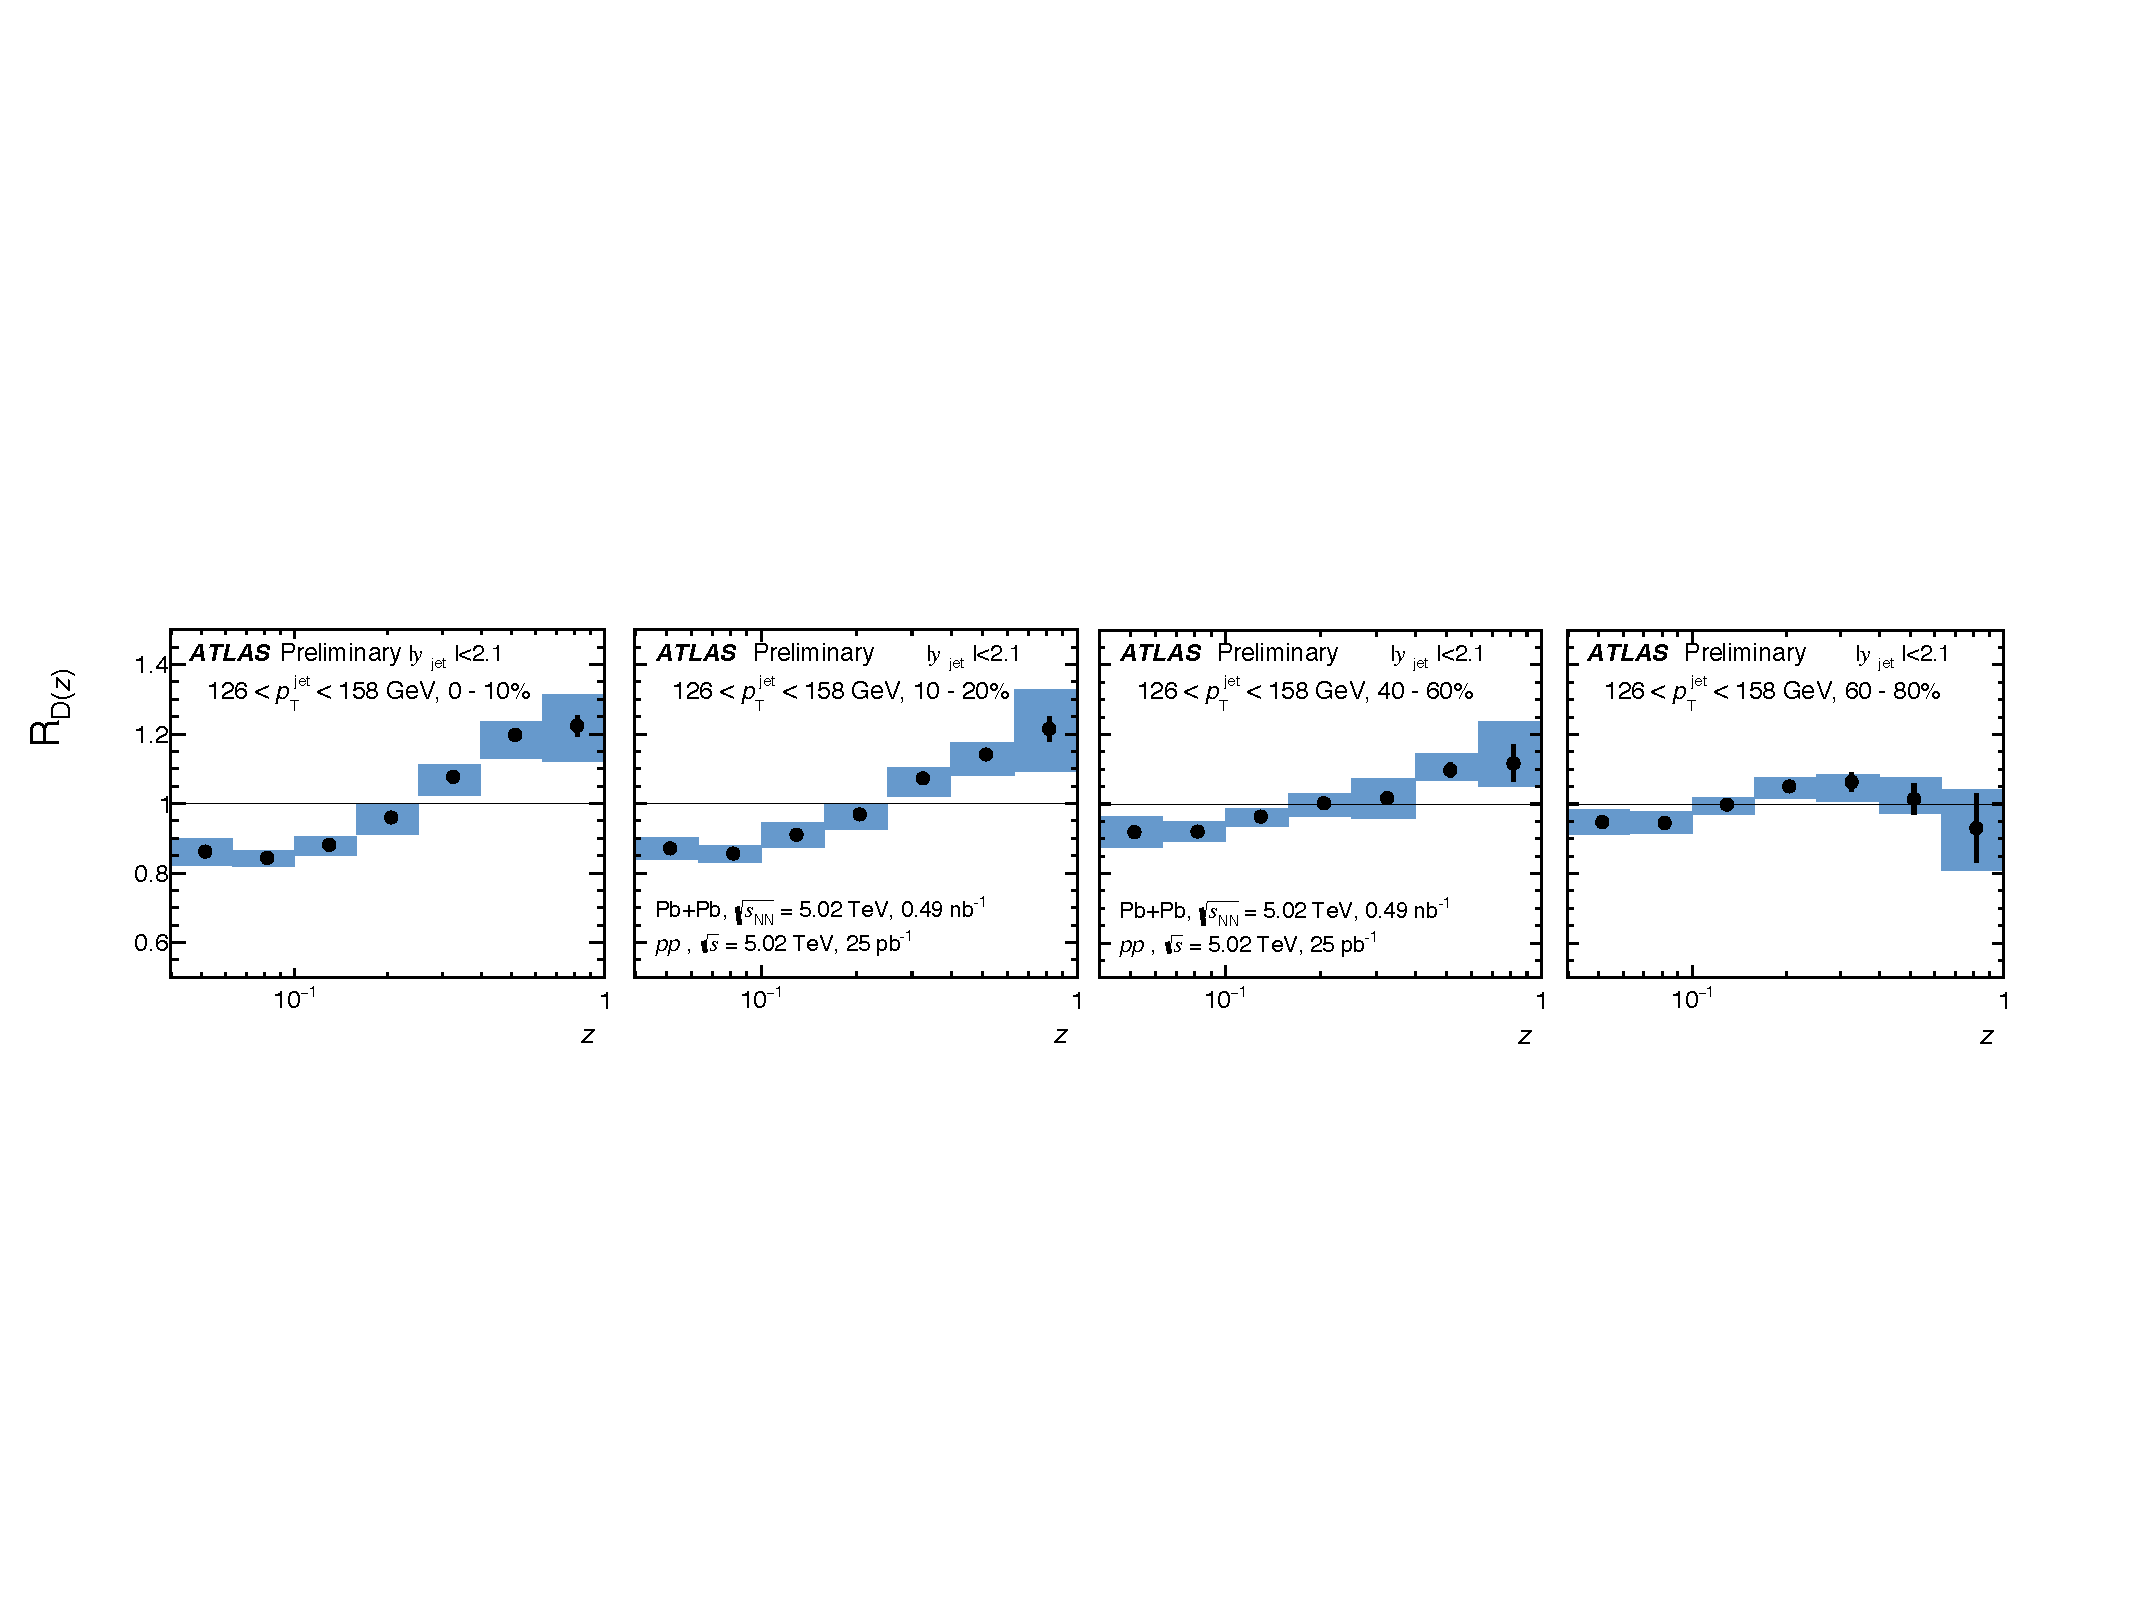
\includegraphics[width=1.0\textwidth]{figures/qualification/ff_502} %
%	\caption{$R_{D(z)}$ as measured by ATLAS at \sqrtsnn\ = 5.02 TeV. The fragmentation function modification monotonically decreases for less central collisions. Taken from \cite{ATLAS-CONF-2017-005}}	
%	\label{fig:ff_502}%
%\end{figure}
%
%There are theory calculations (shown in Fig.~\ref{fig:ff_theory}) that can be compared to data \cite{Casalderrey-Solana:2016jvj}, which while qualitatively have roughly the same shape, but do not describe the data well. Furthermore, calculations of jet energy loss (shown in Fig.~\ref{fig:ff_motivation}), show that a a significant amount of energy is both redistributed, as well as lost outside the jet cone. Combining the fragmentation functions dependence on the longitudinal momentum fraction, with the radial dependence will help constrain theoretical models and give a better understanding of how energy is redistributed around the jet cone, as the jet goes through the quark gluon plasma.
%
%\begin{figure}[!tbp]
%  \centering
%  \begin{minipage}[b]{0.45\textwidth}
%	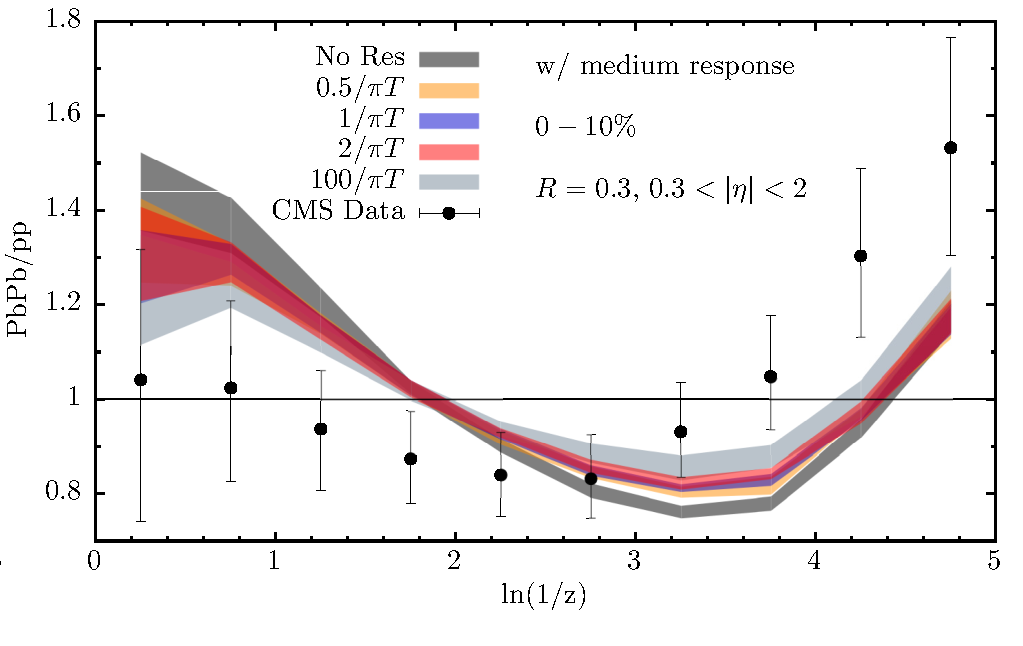
\includegraphics[width=\textwidth]{figures/qualification/ff_theory} %
%	\caption{Theoretical calculations of fragmentation functions as calculated in \cite{Casalderrey-Solana:2016jvj}. They are compared to data from CMS. Note that the x-axis is in $\ln(1/z)$, as opposed to $z$. Taken from \cite{Casalderrey-Solana:2016jvj}}	
%	\label{fig:ff_theory}%
%  \end{minipage}
%  \hfill
%  \begin{minipage}[b]{0.45\textwidth}
%	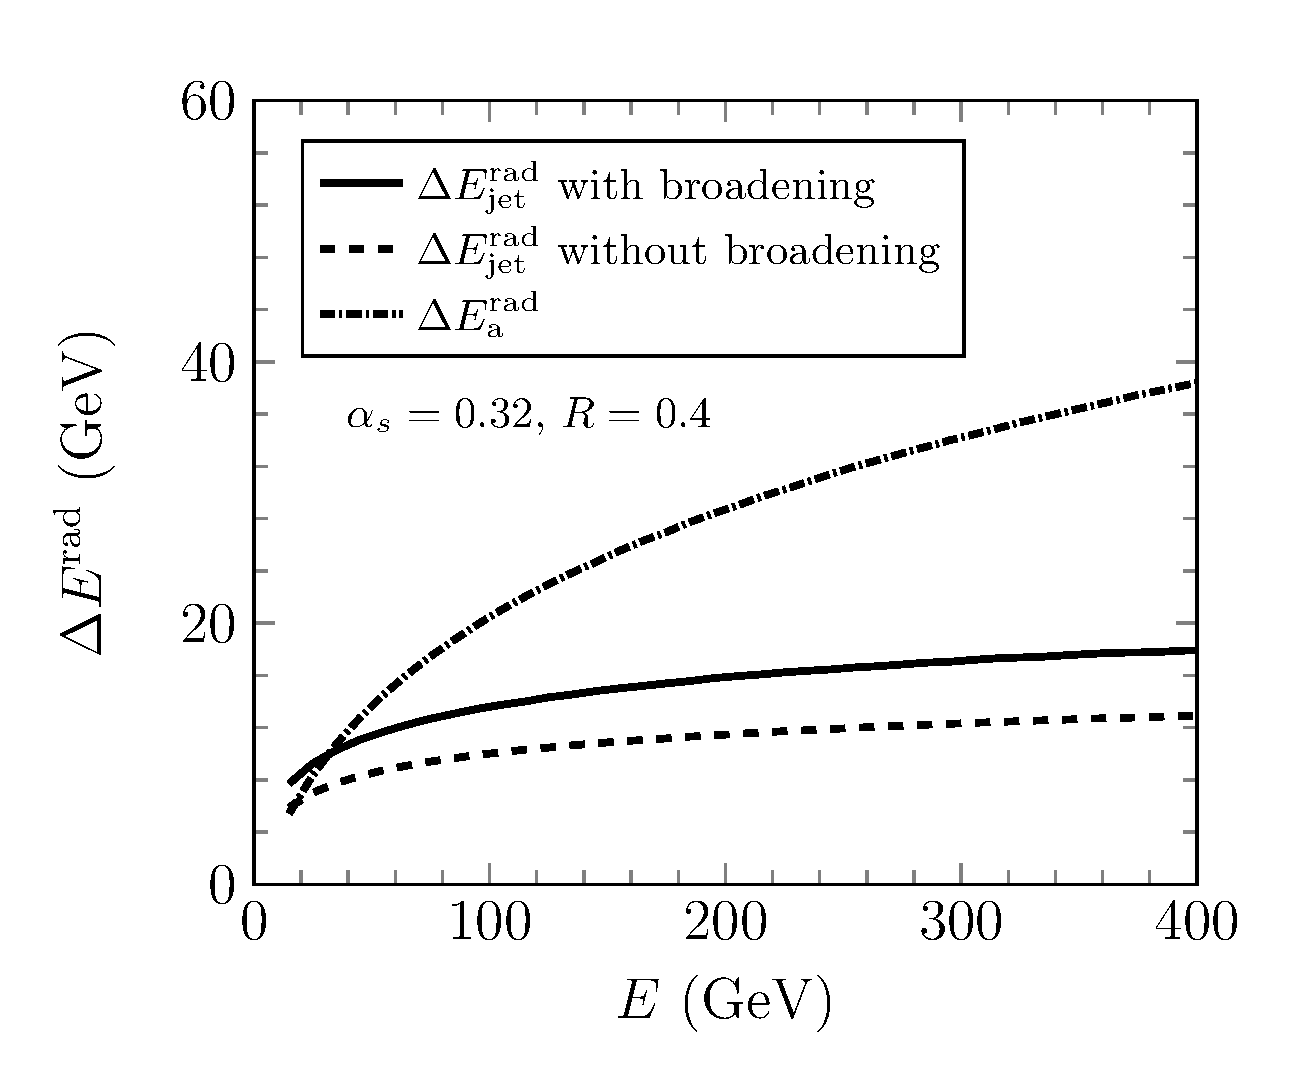
\includegraphics[width=\textwidth]{figures/qualification/ff_motivation} %
%	\caption{$R_{D(z)}$ as measured by ATLAS at \sqrtsnn\ = 5.02 TeV. The fragmentation function modification monotonically decreases for less central collisions. Taken from \cite{ATLAS-CONF-2017-005}}	
%	\label{fig:ff_motivation}%
%  \end{minipage}
%\end{figure}
